\documentclass[a4paper,english,12pt,bibliography=totoc]{scrreprt}

\usepackage[
backend=biber,
style=alphabetic,
sorting=ynt
]{biblatex}

\addbibresource{Bioinformatics Report.bib}
\bibliography{Bioinformatics Report}
\usepackage[T1]{fontenc} %immer
\usepackage[utf8]{inputenc} %am
\usepackage{babel} %Anfang

\usepackage{enumitem} %Aufzählungen verändern

%Gleichungen verwenden
\usepackage{newtxtext}
\usepackage{amsmath}
\usepackage{amssymb}
\usepackage{mathptmx}
%\usepackage{txfonts}

\usepackage{listings}% code blocks
\usepackage[most]{tcolorbox}

%Querverweise
\usepackage{varioref} %immer
\usepackage{hyperref} %in dieser
\usepackage{cleveref} %Reihenfolge

\usepackage{booktabs} %schönere Tabellen
\usepackage{siunitx} %SI-Einheiten
\usepackage{tabularx} %Tabellen mit flexiblen Spalten	

\usepackage{graphicx} %Grafiken verwenden

\usepackage{lipsum} %Blindtext
\usepackage{subcaption}
\usepackage{afterpage}
\usepackage[headsepline]{scrlayer-scrpage} %Paket für Kopfzeilen
\usepackage{afterpage}
\usepackage{float}
\automark[subsection]{section}

\pagestyle{scrheadings}
\ihead{} % oben links
\chead{\leftmark} % oben Mitte
\ohead{} % oben rechts
\cfoot{\pagemark} % unten Mitte
\automark[section]{section} % Modified line

% Zu volle hboxen korrigieren
\tolerance 1414
\hbadness 1414
\emergencystretch 1.5em
\hfuzz 0.3pt
\widowpenalty=10000
\vfuzz \hfuzz
\raggedbottom

%Informationen über das Dokument
\date{\today}


\begin{document}


\begin{titlepage}
	\centering
	
\includegraphics[width=0.8\textwidth]{logo_uulm_sw}
	
	\vspace{1cm}
	\LARGE Laboratory Module for Master Programs
	\Huge \textbf{Biophysics Lab Course}
	
	\vspace{1cm}
	\Large Experiment:

	\Huge \textbf{Bioinformatics}
	
	\vspace{15mm}
	\Large Performed on 
	
	\vspace{5mm}
	\LARGE Group 8
	
	\vspace{1cm}
	\Large
	\begin{tabular}{rcl}
	\textbf{Haiyang Zhang} & and & \textbf{Nicolae Turcan}\\
	\href{mailto:student.1@uni-ulm.de}{haiyang.zhang@uni-ulm.de} & & \href{mailto:student.2@uni-ulm.de}{nicolae.turcan@uni-ulm.de}
	\end{tabular}
	
	\vspace{7mm}
	Supervisor: Camilla Förster
	
	\vfill
	\begin{tabular}{p{50mm}@{\hspace{5cm}}p{50mm}}
	\hrulefill & \hrulefill \\
	%\centering Haiyang Zhang  & \centering Nicolae Turcan
	\end{tabular}
	
	\vspace{5mm}
	\normalsize \raggedright
	We hereby confirm that we have elaborated the present work independently and have detailed knowledge of the entire contents.
\end{titlepage}



\tableofcontents

\begin{comment}
\chapter{Abstract}
\label{cha:abstract}

\chapter{Introduction}
\label{cha:Introduction}



\chapter{Material and Methods}
\label{cha:MaterialandMethods}

\section{Material}
\label{sec:material}

\section{Methods}
\label{sec:methods}


\chapter{Experiment and Analysis}
\label{cha:experimenandanalysis}  

\section{Experiment}
\label{sec:experiment} 

\section{Analysis}
\label{sec:analysis} 



\chapter{Results and Discussion}
\label{cha:ResultsandDiscussion}

\section{Results}
\label{sec:Results} 

\section{Discussion}
\label{sec:Discussion} 




\chapter{Conclusion}
\label{cha:Conclusion}

\chapter{References}
\label{cha:References}
\end{comment}

\chapter{Project 1}
In the following section we will display the results of the first project of the bioinformatics laboratory.
The objective of the first project was to identify an unkown protein from short peptide sequences given in Table 1.1 .
The project consisted in doing 5 BLAST searches , which allows you to search a database for similar sequences. It works by identifying regions of similarity between our query and sequences in the database, assigning scores based on similarity and statistical significance. The results provide a list of sequences from the database that closely match our query [\cite{altschul_basic_1990}].

\section{results}

\begin{table}[H]
\centering
\begin{tabular}{|l|l|}
\hline
\textbf{Peptide Sequence 1} & TVGWIAHWSEMHSDGMK \\
\hline
\textbf{Peptide Sequence 2} & AMGIPSSMFTVIFAMAR \\
\hline
\textbf{Reverse Peptide Sequence 2} & RAMAFIVTFMSSPIGMA \\
\hline
\end{tabular}
\caption{Peptide sequences}
\end{table}


\subsection{1st BLAST search }
The first BLAST search was performed on Peptide Sequence 1 displayed in Table 1.1.
The results of this BLAST search are displayed in three parts:

A Graphic summary( Figure 1.1) displaying  a distribution of the best esntries in comparison with the query sequence, the aminoacid position is signed as well to enable better comparison, the color green signifies a similarity of over 90 percent.
\begin{figure}[H]
    \centering
    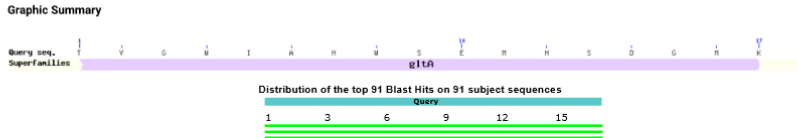
\includegraphics[width=0.9\linewidth]{Project 1/graphicsummary1.png}
    \caption{Graphic summary of Top 3 results in 1st BLAST search}
    \label{fig:enter-label}
\end{figure}

The Description table in Figure 1.2  submits the sequence of origin and the organism name from which it the sequence was isolated, following that we have multiple parameters that can help us better choose which sequence of origin is more suitable and  in particular an E value. The E-value, or Expectation value, refers to the number of random matches one can expect to find by chance when searching a database with a particular query, a lower E-value indicates a more significant match. 

\begin{figure}[H]
    \centering
    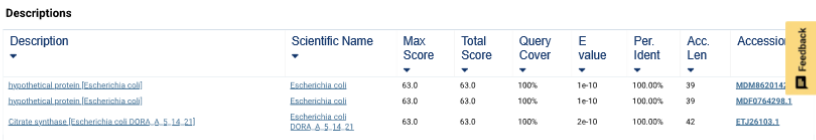
\includegraphics[width=0.9\linewidth]{Project 1/Description1.png}
    \caption{Top 3 results of 1st BLAST search}
    \label{fig:enter-label}
\end{figure}

And finally , in Figure 1.3 we can see a detailed set of pairwise alignements bewteen the query and the best candidates, in this case the 3rd candidate provided the most significant result with information on the function of the protein in which it was found.

\begin{figure}[H]
    \centering
    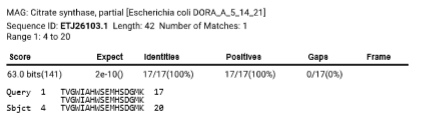
\includegraphics[width=0.9\linewidth]{Project 1/AlignedSequence.png}
    \caption{3rd Alignment of 1st BLAST search}
    \label{fig:enter-label}
\end{figure}

The Following BLAST search results will be displayed in the same order and without further comment if not necessary.

\subsection{2nd BLAST search }

\begin{figure}[H]
    \centering
    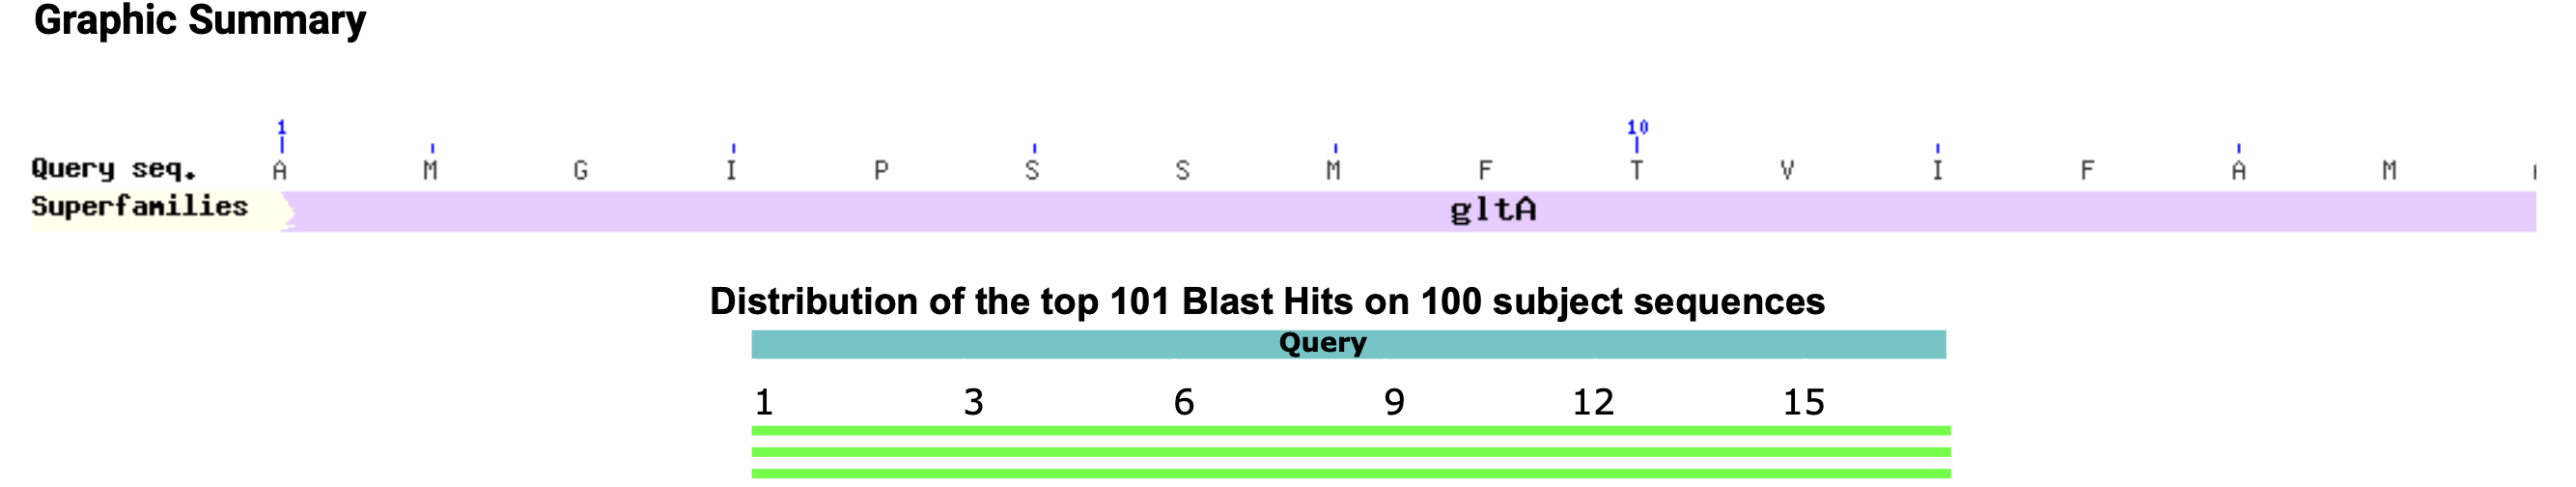
\includegraphics[width=0.9\linewidth]{Project 1/2nd Images/graphic summary.png}
    \caption{Graphic summary of Top 3 results in 2nd BLAST search}
    \label{fig:enter-label}
\end{figure}


\begin{figure}[H]
    \centering
    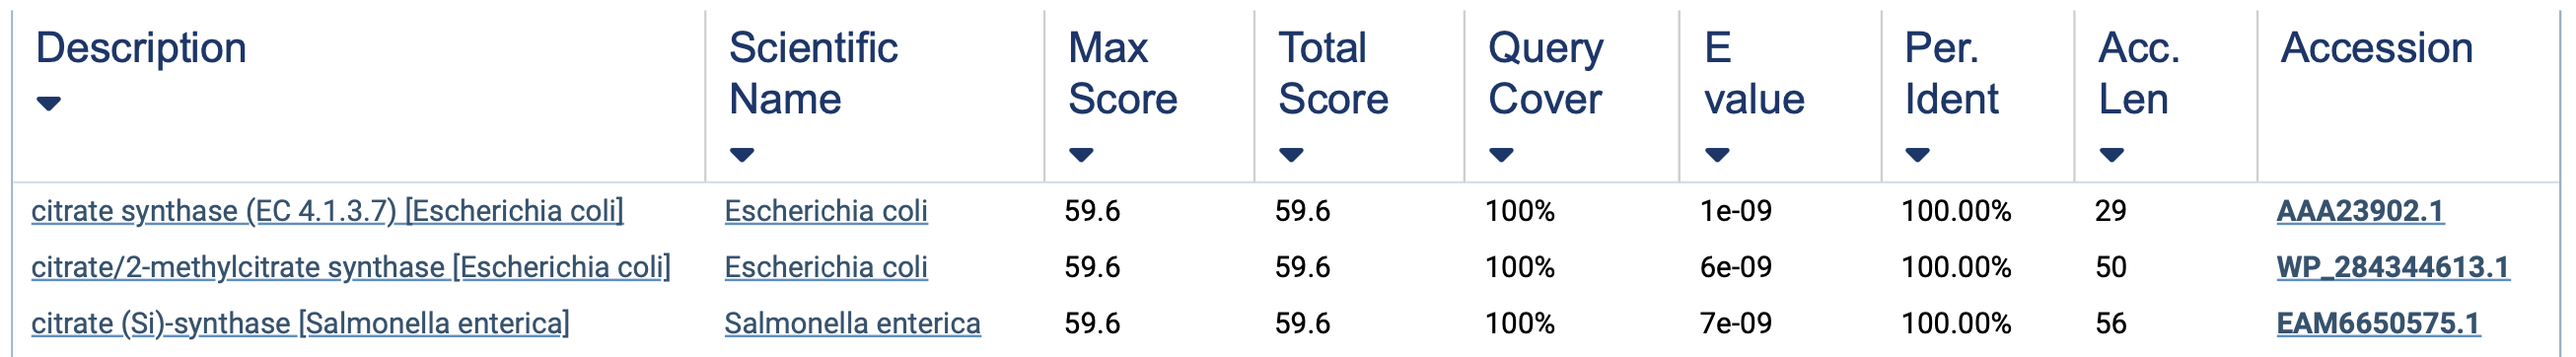
\includegraphics[width=0.9\linewidth]{Project 1/2nd Images/Blast results.png}
    \caption{Top 3 results of 2nd BLAST search}
\end{figure}


\begin{figure}[H]
    \centering
    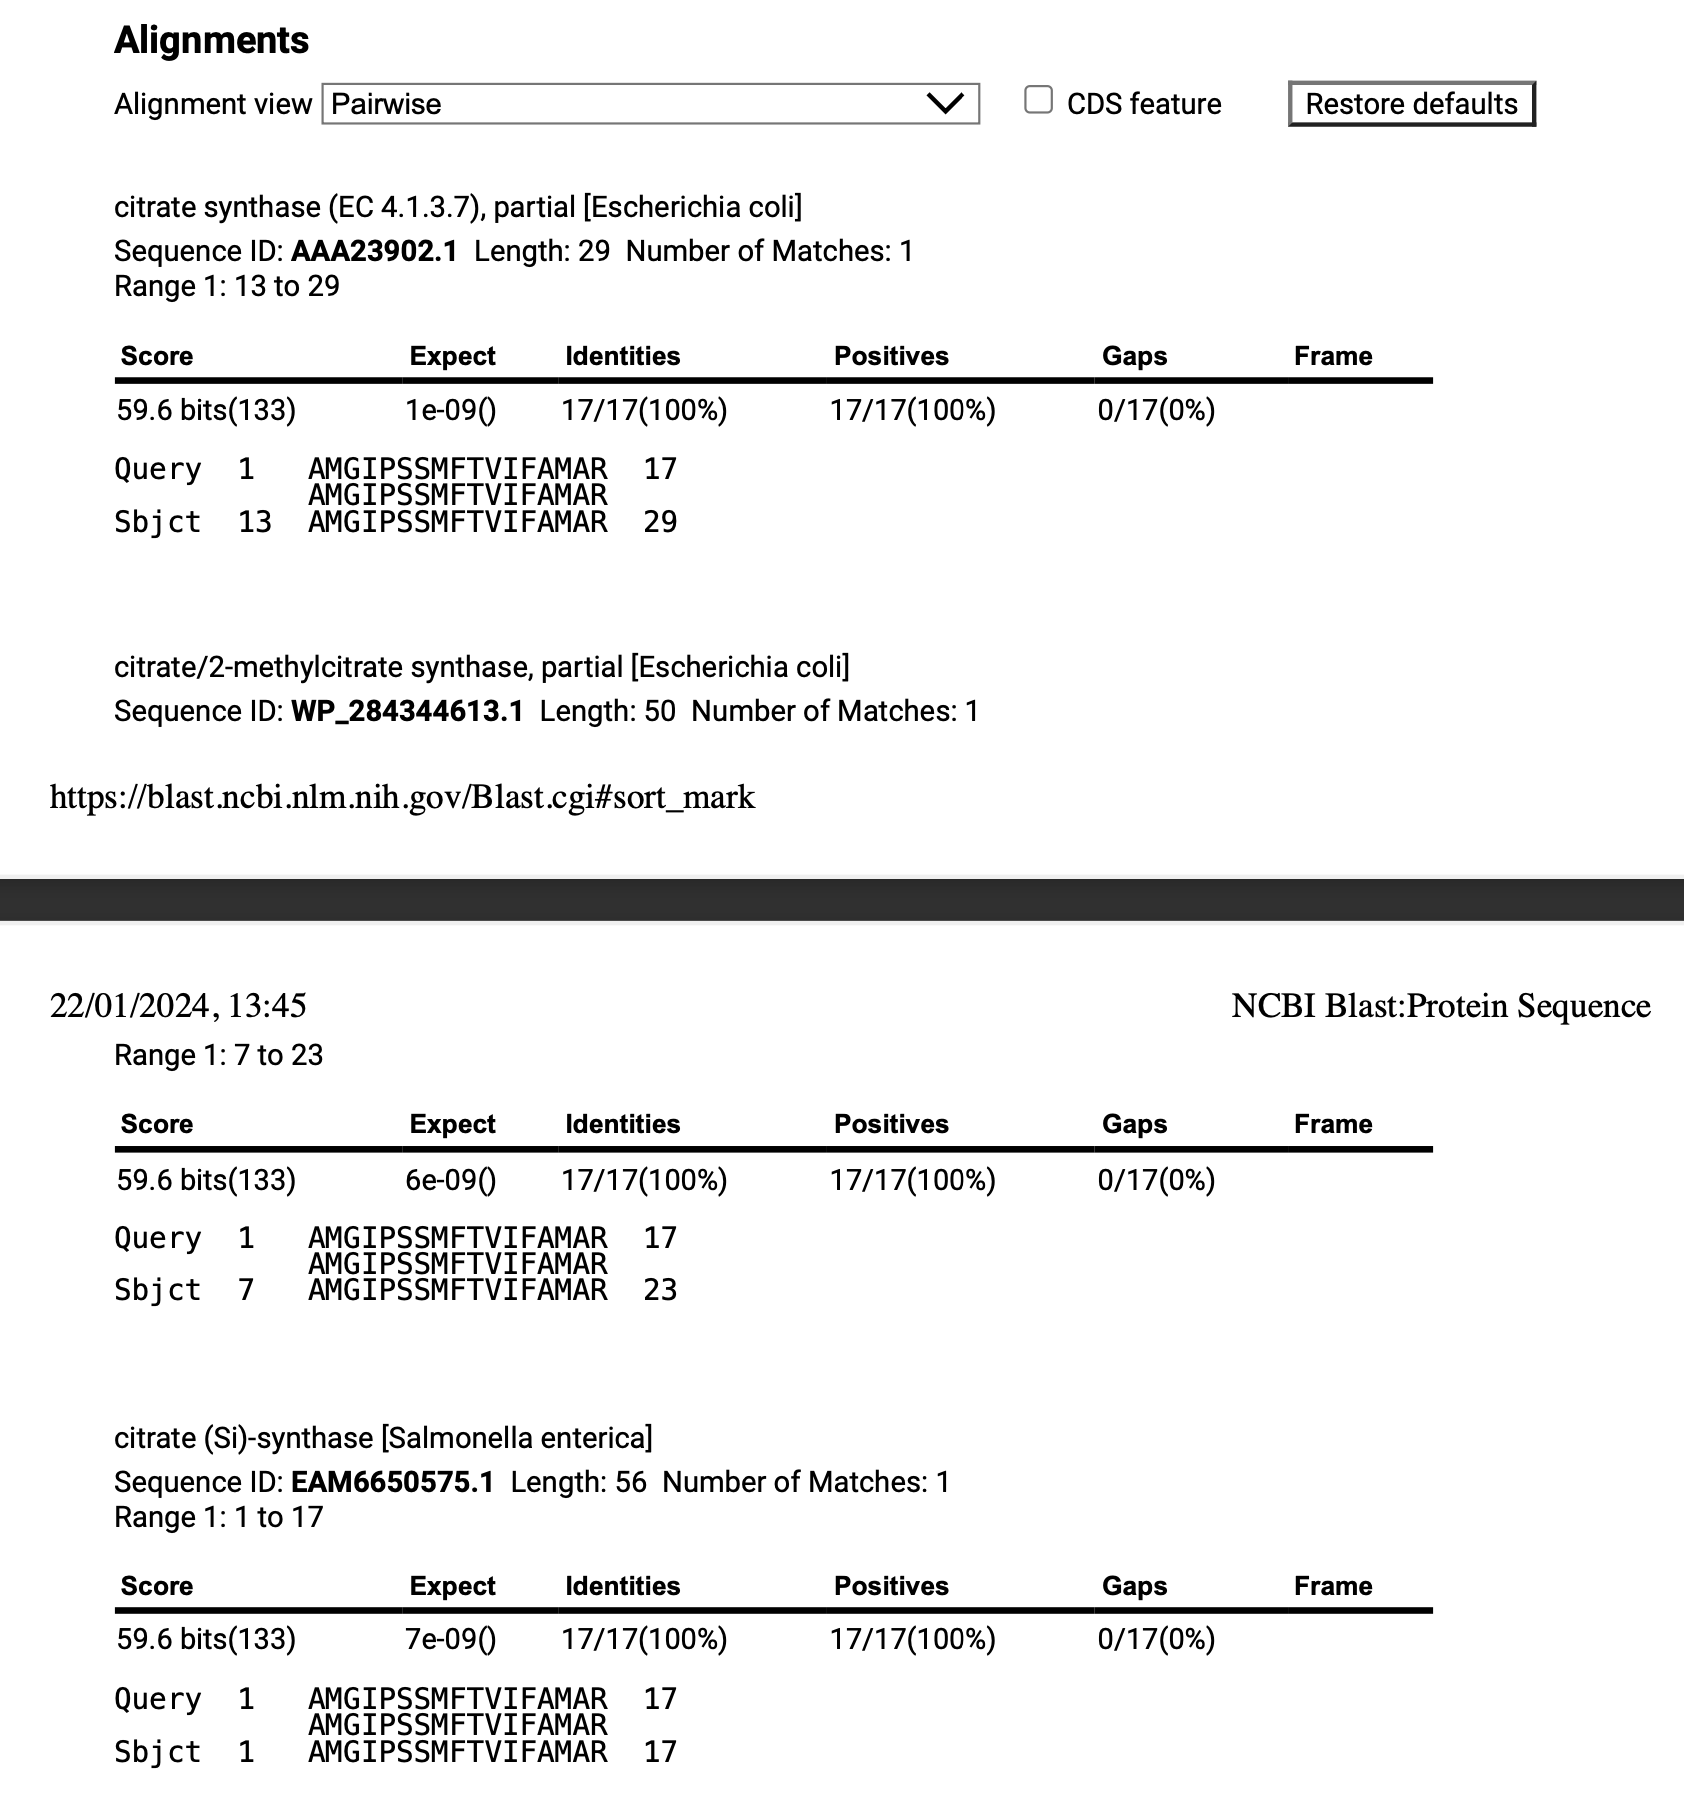
\includegraphics[width=0.9\linewidth]{Project 1/2nd Images/Alignments.png}
    \caption{Top 3 Alignments of 2nd BLAST search}
    \label{fig:enter-label}
\end{figure}

\subsection{3rd BLAST search}

\begin{figure}[H]
    \centering
    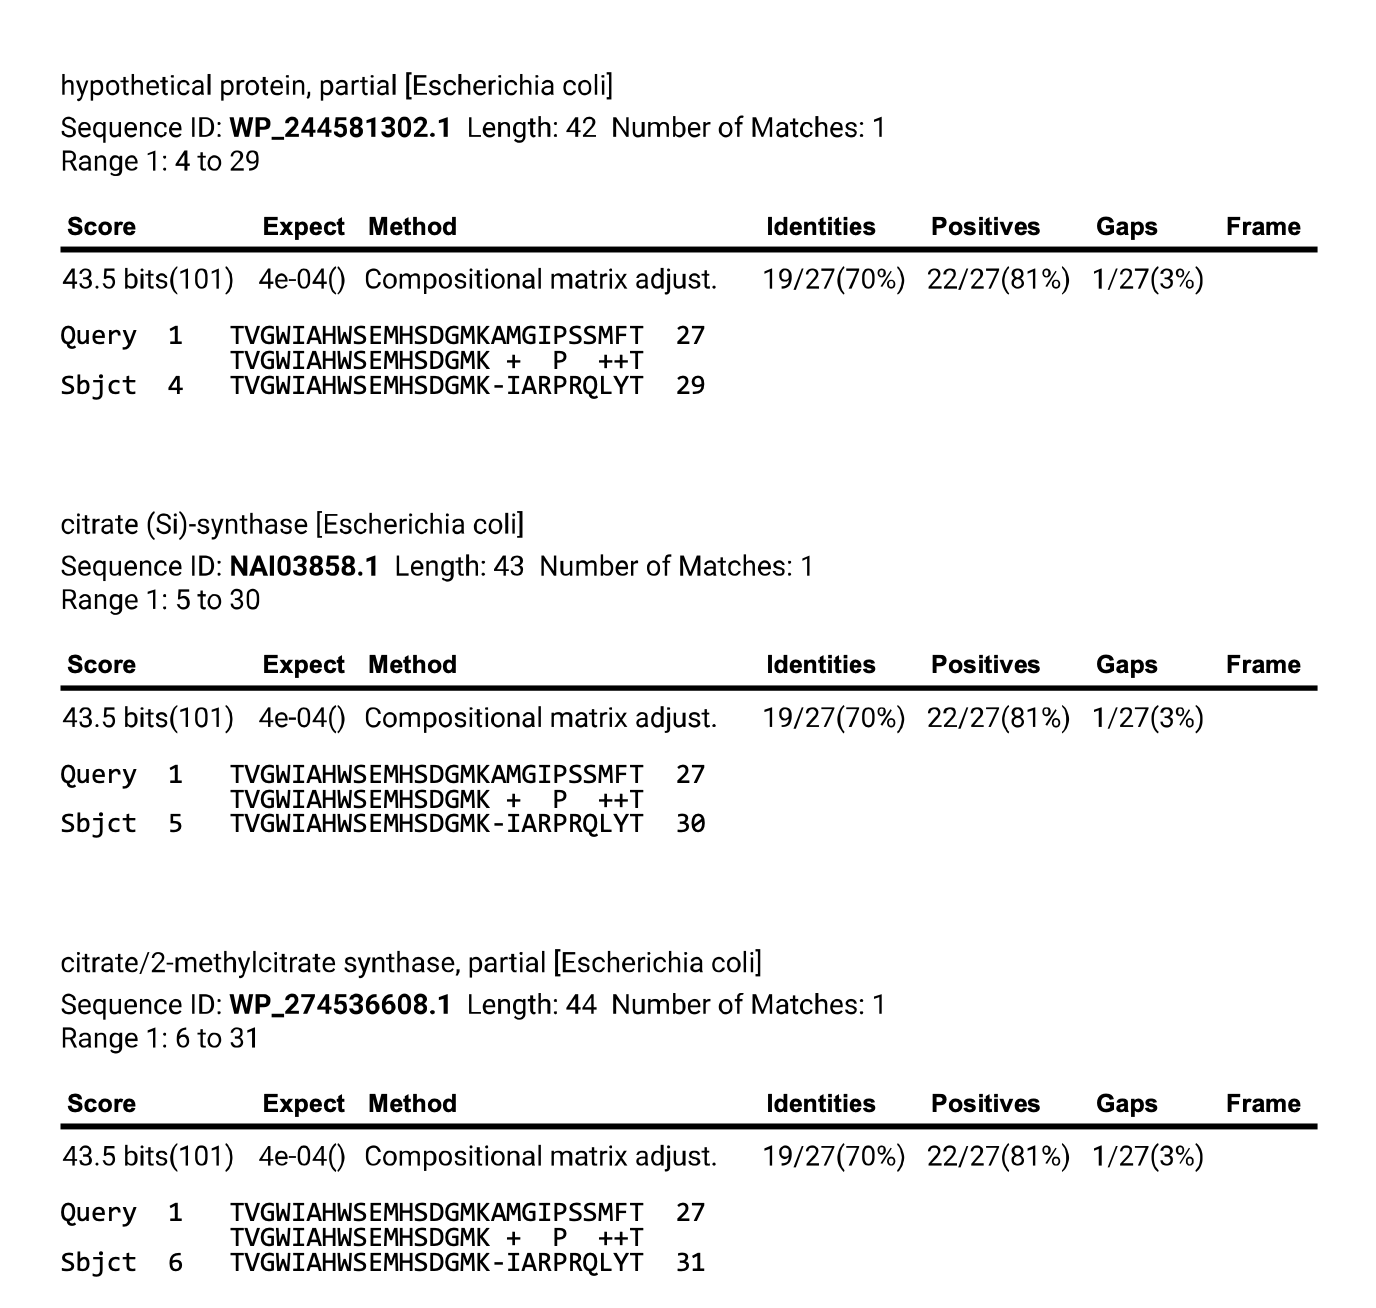
\includegraphics[width=0.9\linewidth]{Project 1/3rd images/alignments 3.png}
    \caption{Top 3 alignments of 3rd BLAST search}
    \label{fig:enter-label}
\end{figure}

\begin{figure}[H]
    \centering
    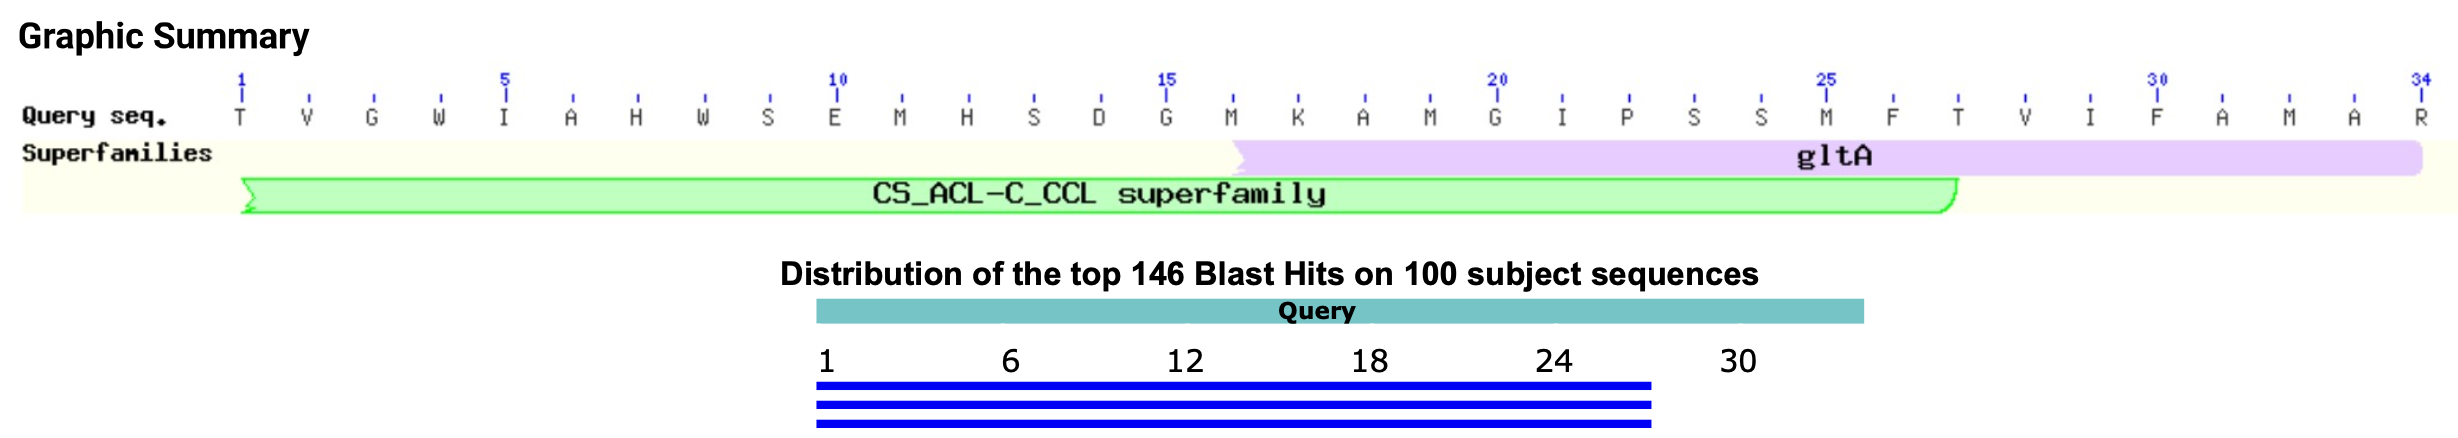
\includegraphics[width=0.9\linewidth]{Project 1/3rd images/graphic summary 3.png}
    \caption{Graphic summary of Top 3 results in 3rd BLAST search}
    \label{fig:enter-label}
\end{figure}


\begin{figure}[H]
    \centering
    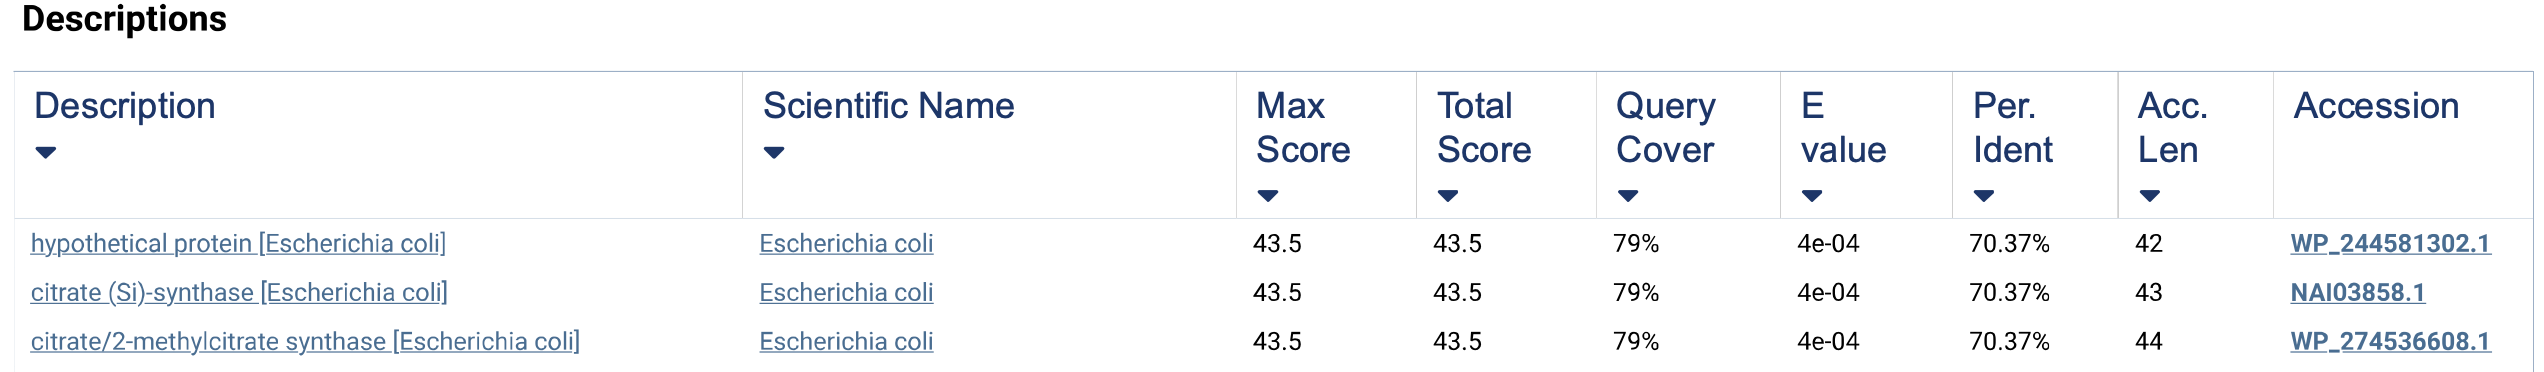
\includegraphics[width=0.9\linewidth]{Project 1/3rd images/Blast results 3.png}
    \caption{Top 3 results of 3rd BLAST search}
    \label{fig:enter-label}
\end{figure}


\subsection{4th BLAST search}

\begin{figure}[H]
    \centering
    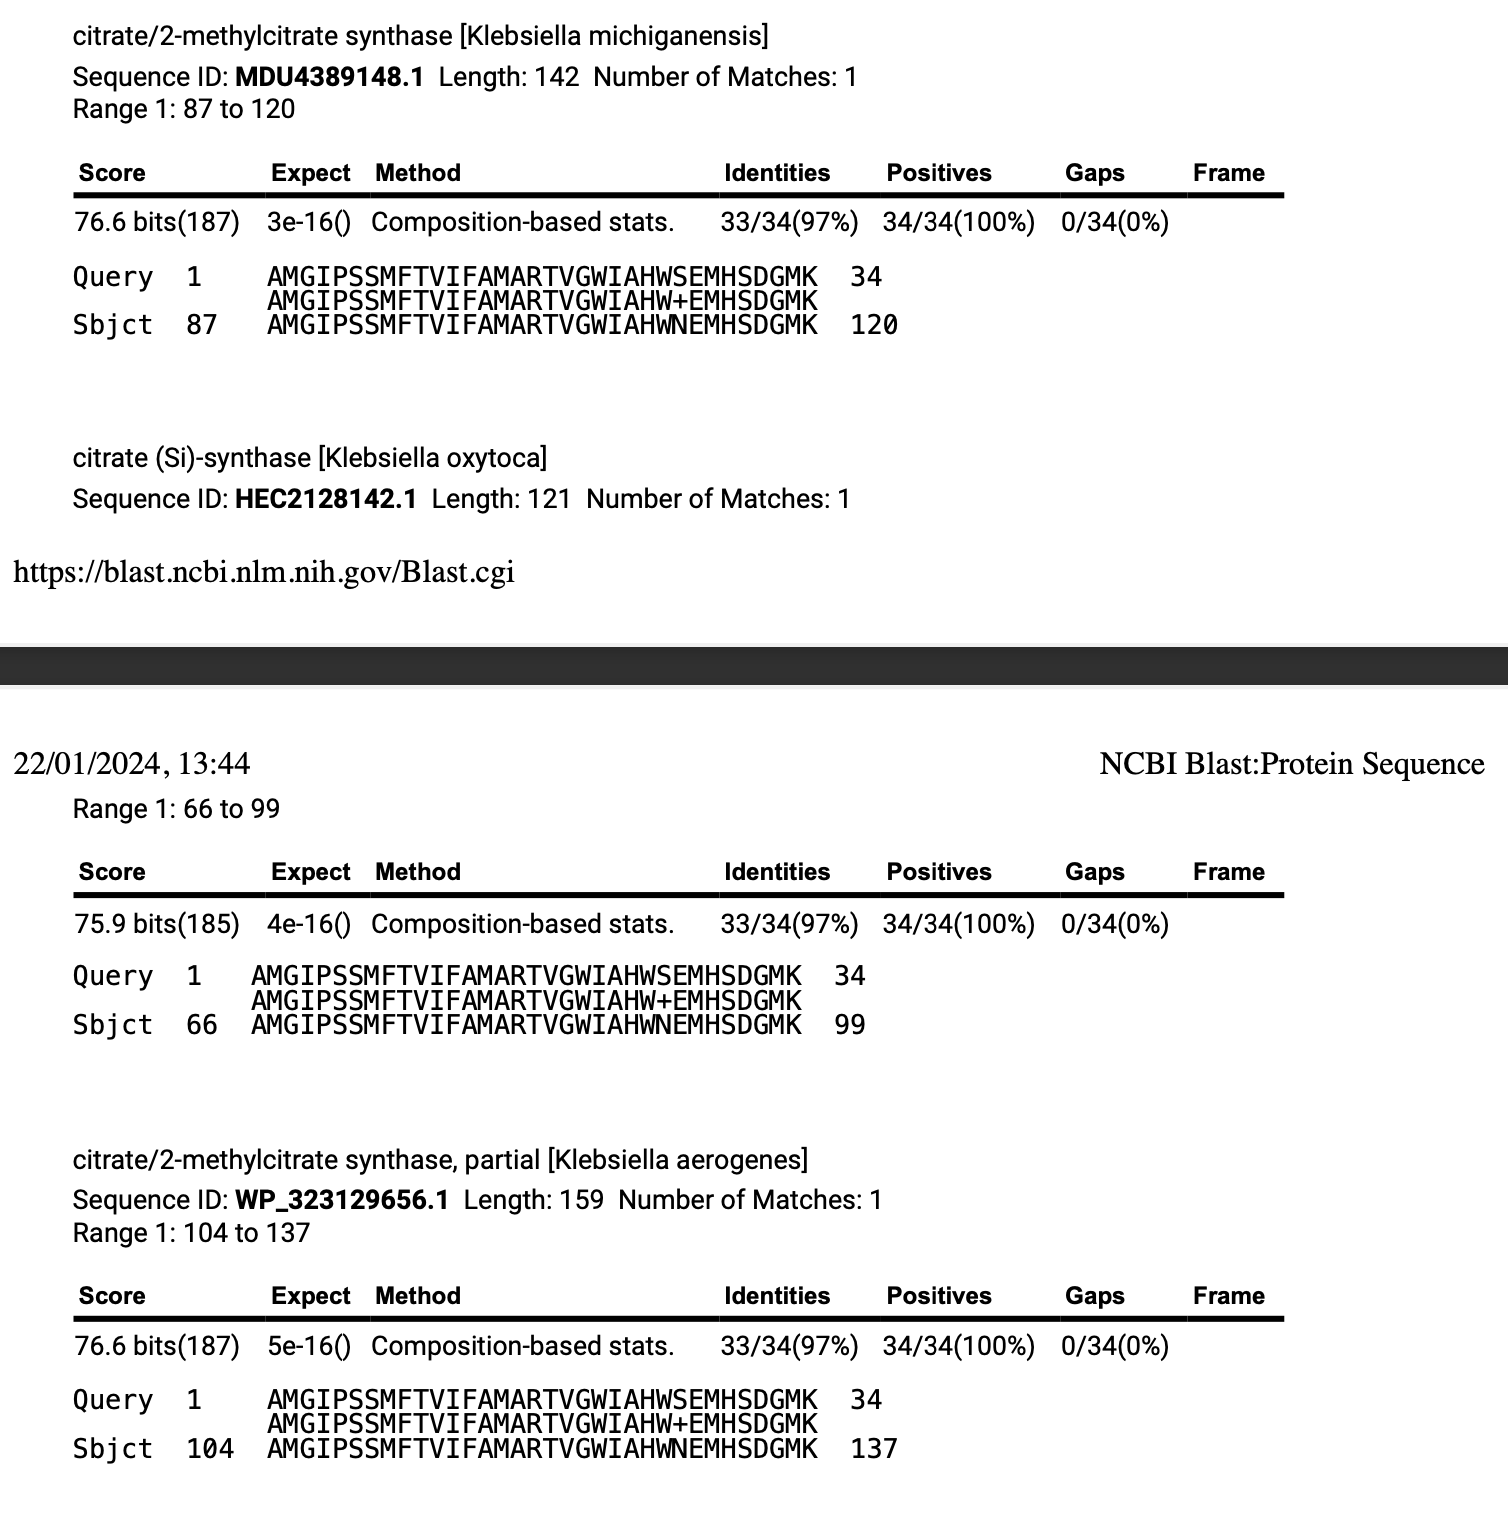
\includegraphics[width=0.9\linewidth]{Project 1/4th images/alignments 4.png}
    \caption{Top 3 alignments of 4th BLAST search}
    \label{fig:enter-label}
\end{figure}


\begin{figure}[H]
    \centering
    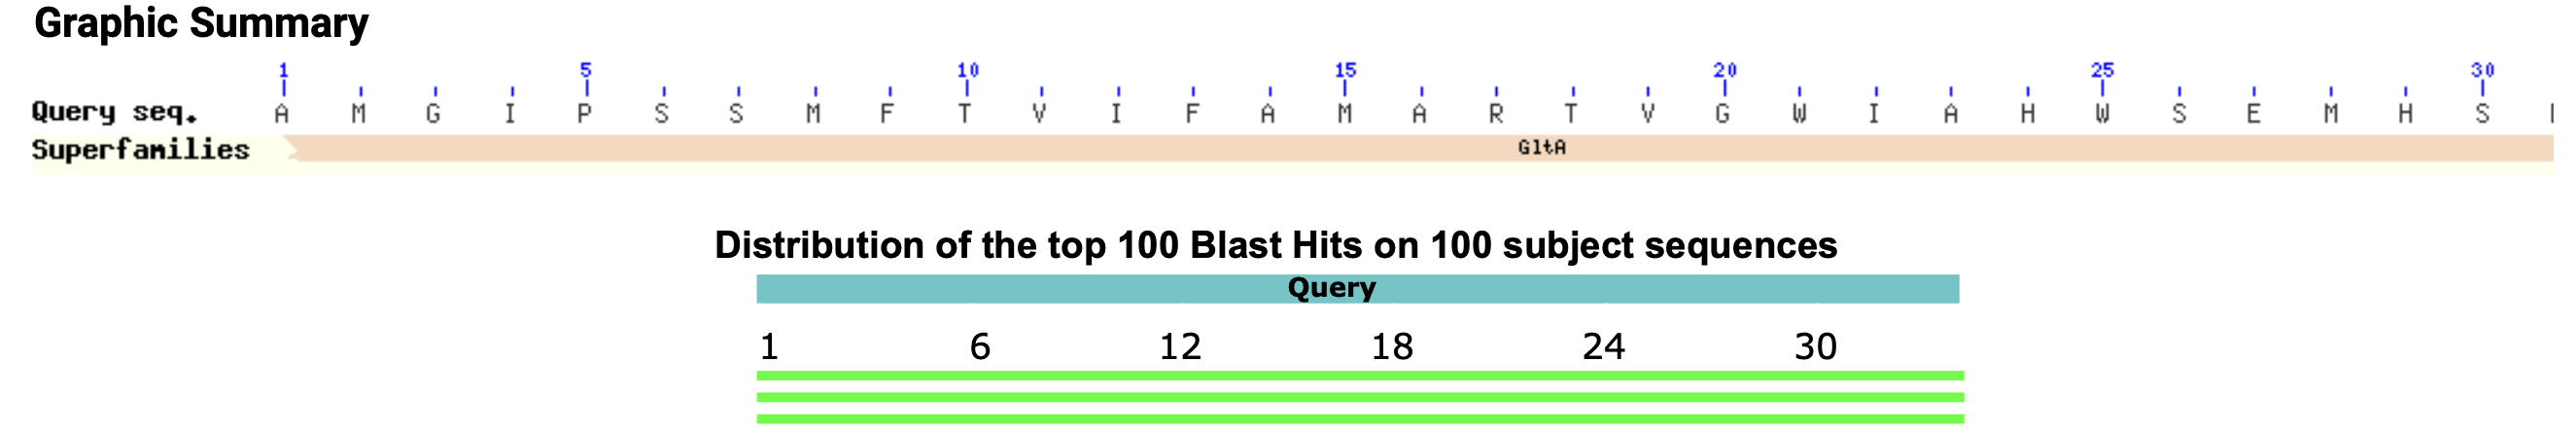
\includegraphics[width=0.9\linewidth]{Project 1/4th images/graphic summary 4.png}
    \caption{Graphic summary of Top 3 results in 4th BLAST search}
\end{figure}


\begin{figure}[H]
    \centering
    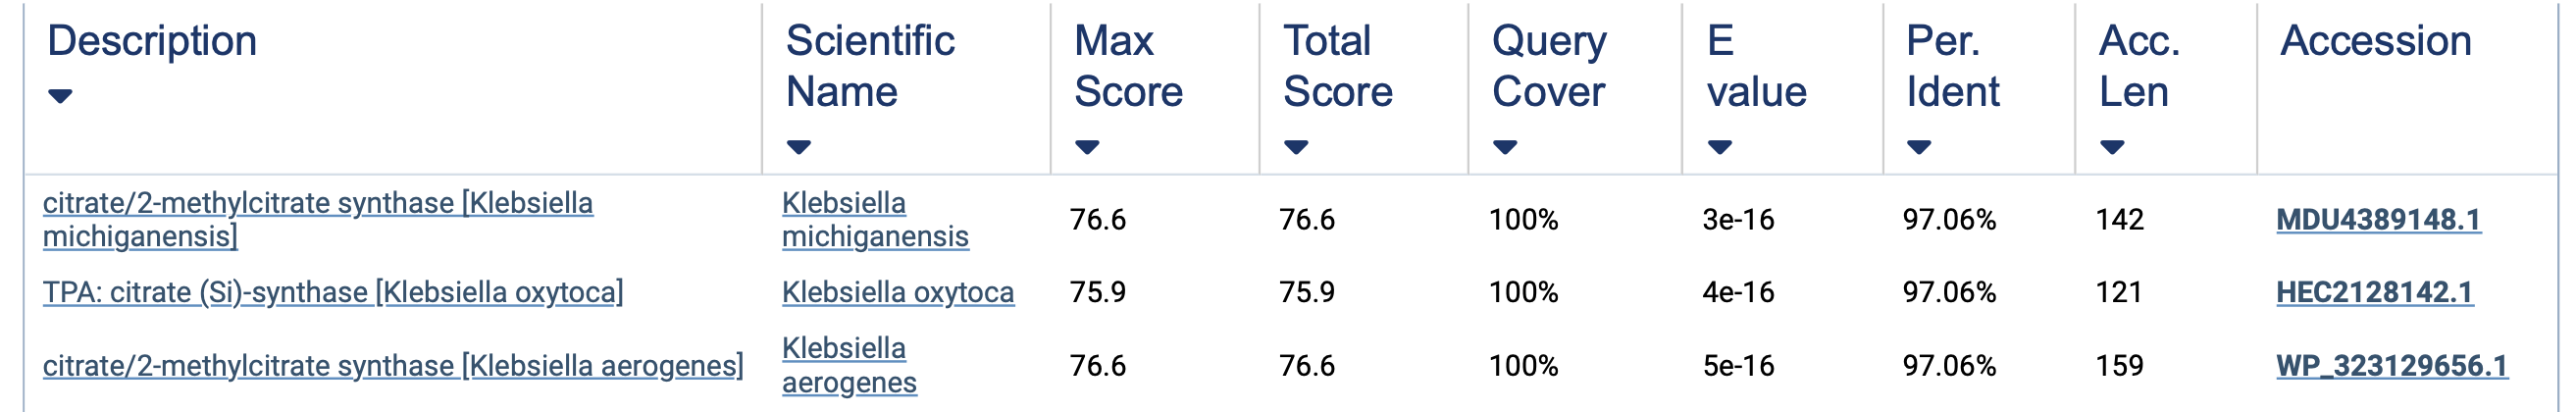
\includegraphics[width=0.9\linewidth]{Project 1/4th images/Blast results 4.png}
    \caption{Top 3 results of 4th BLAST search}
    \label{fig:enter-label}
\end{figure}




\subsection{5th BLAST search}

\begin{figure}[H]
    \centering
    
\includegraphics[width=0.9\linewidth]{Project 1/5th images/graphic summary 5.png}
    \caption{Graphic summary of Top 3 results in 5th BLAST search}
    \label{fig:enter-label}
\end{figure}



\begin{figure}[H]
    \centering
    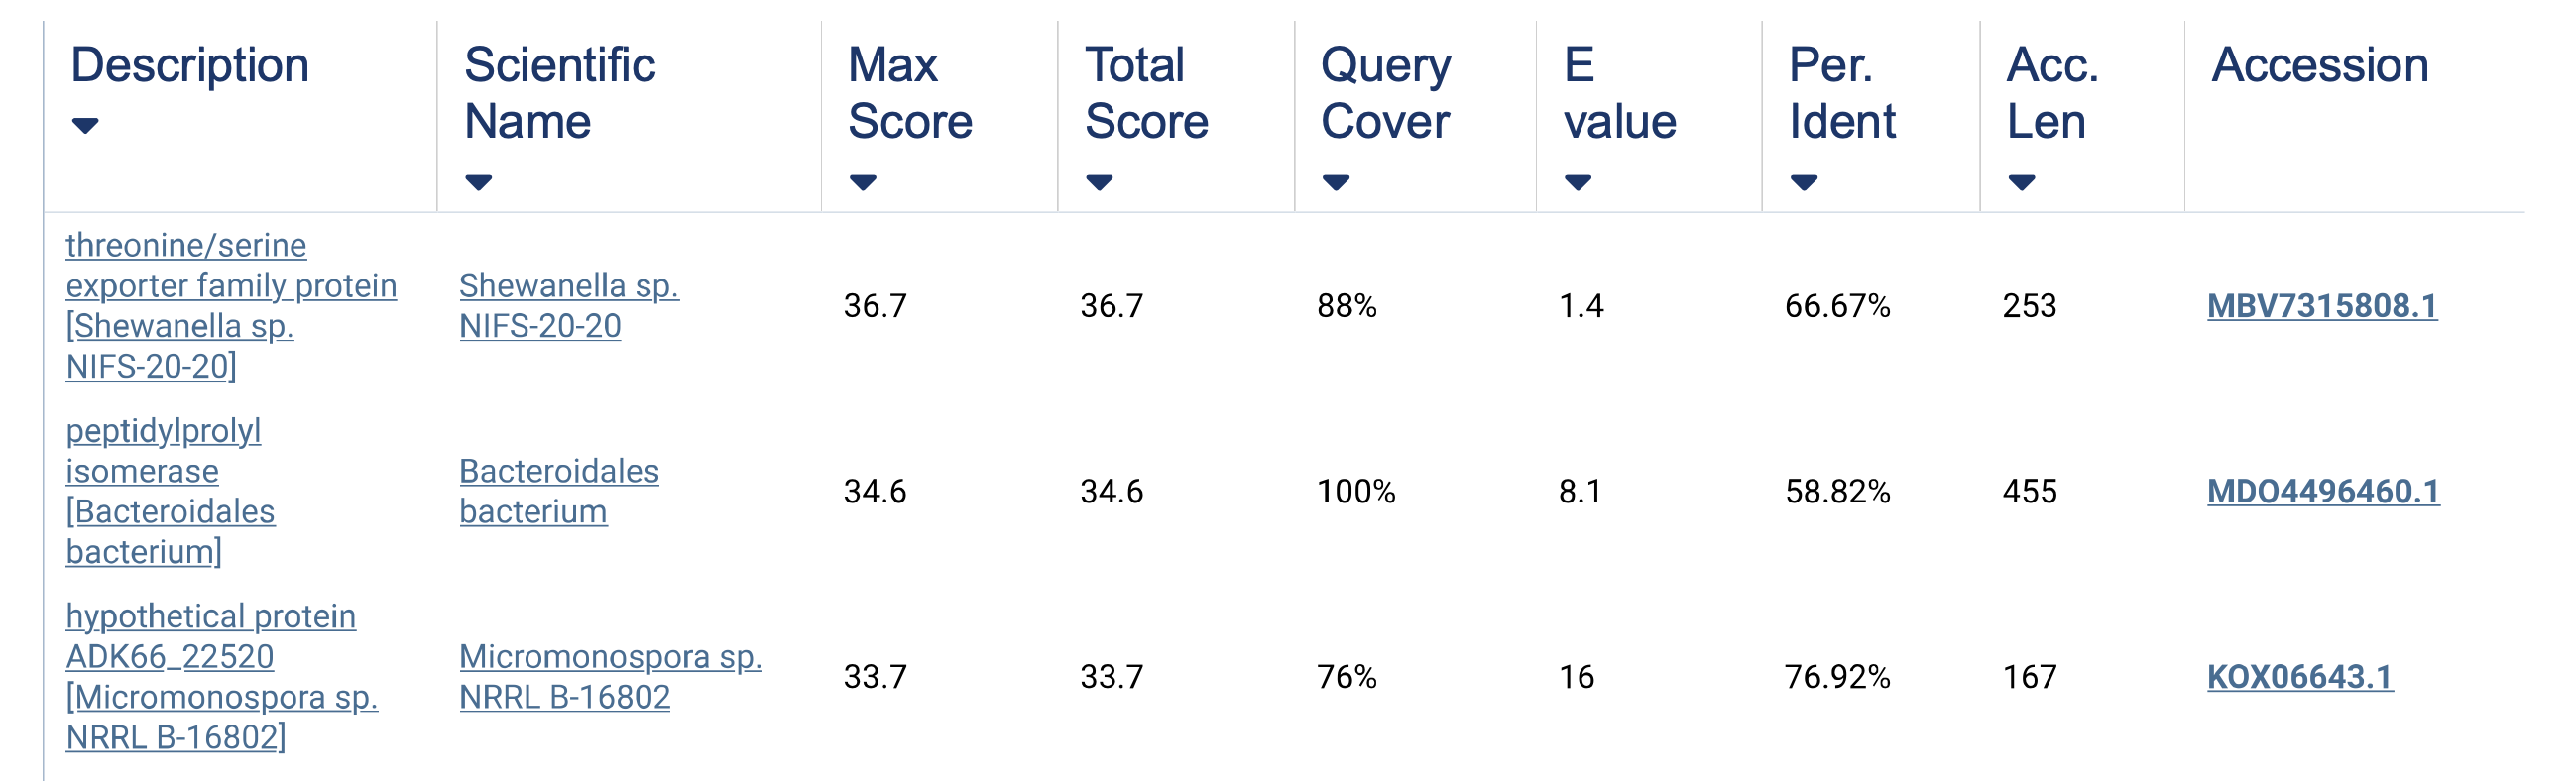
\includegraphics[width=0.9\linewidth]{Project 1/5th images/Blast results 5.png}
    \caption{Top 3 results of 5th BLAST search}
    \label{fig:enter-label}
\end{figure}



\begin{figure}[H]
    \centering
    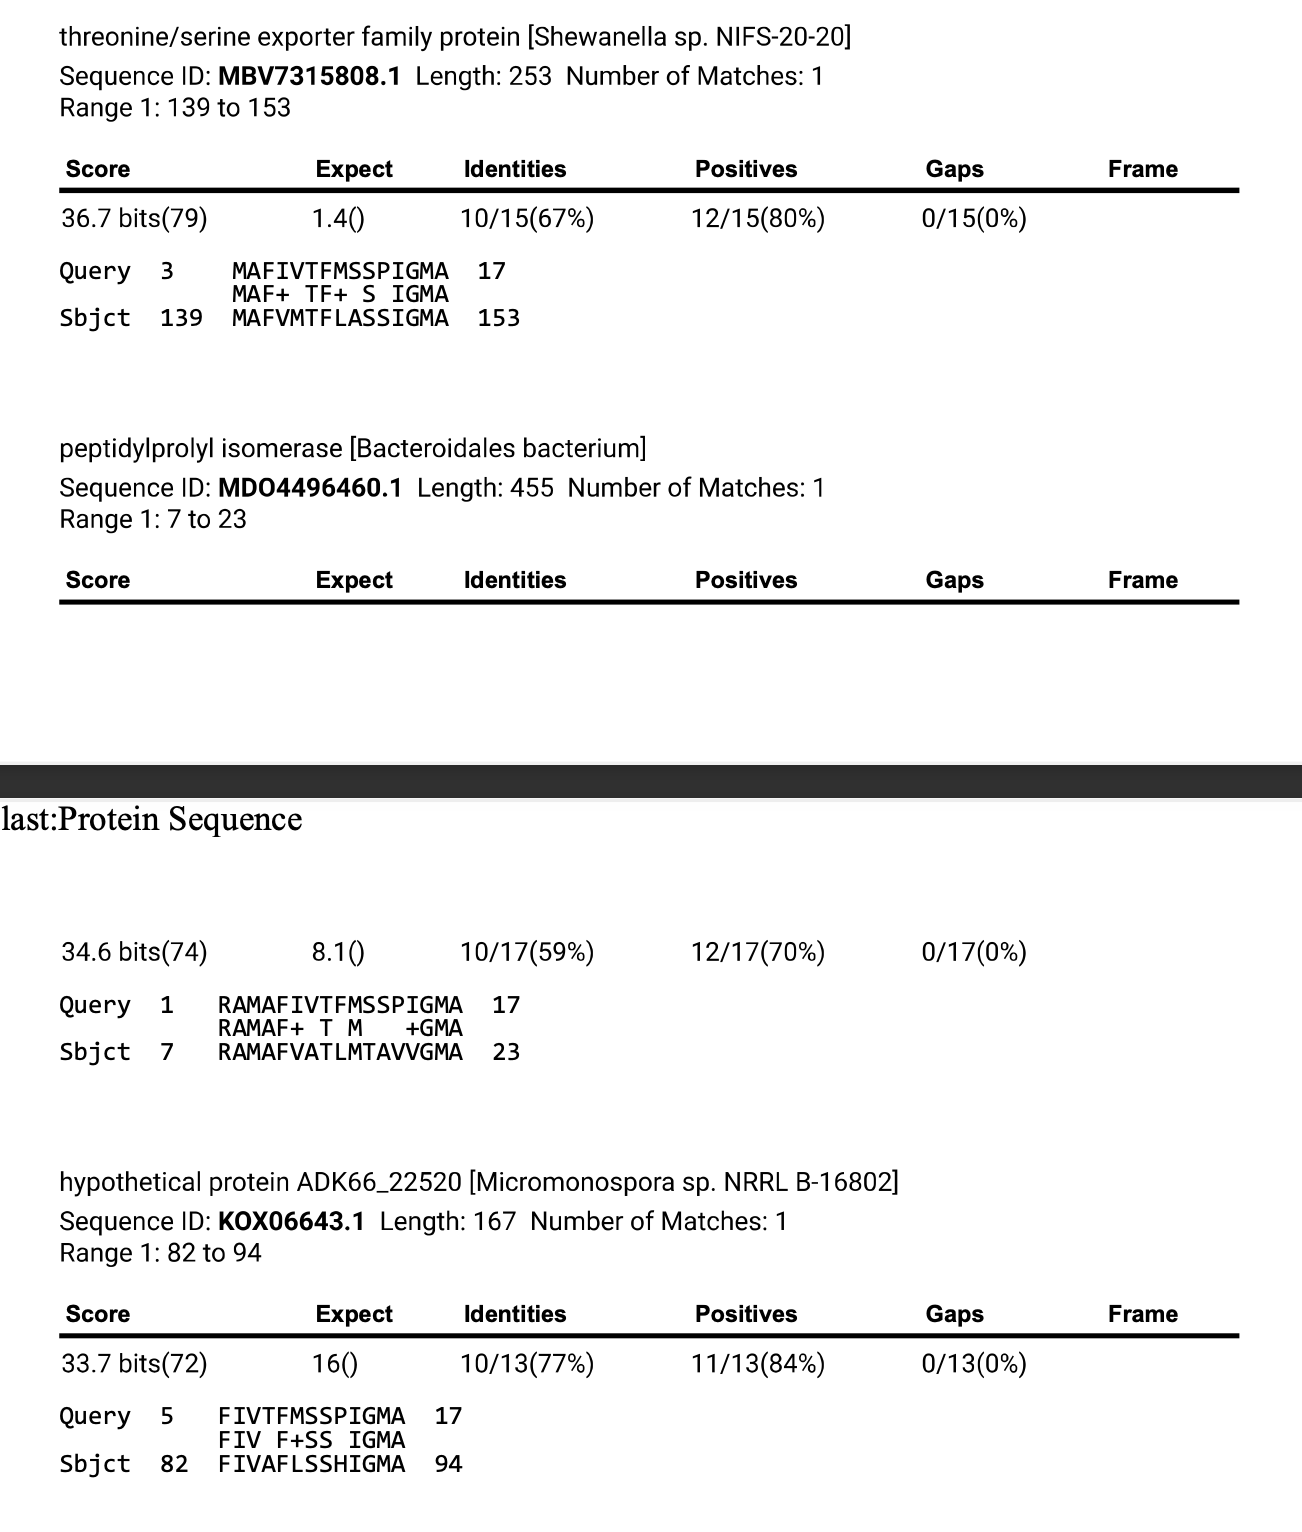
\includegraphics[width=0.9\linewidth]{Project 1/5th images/alignments 5.png}
    \caption{Top 3 alignments of 5th BLAST search}
    \label{fig:enter-label}
\end{figure}



% \subsection{E.C. number and full amino acid sequence of the protein}


\section{discussions}

a) The name of our protein is : 2-Methyl Citrate Synthase.\\

b) There are multiple hits because the same enzyme exists in different organisms, and since most of the results were from bacteria, we can expect to find this protein not only in organisms which performed vertical gene transfer and differentiation in different species, but also in evolutionarly unrelated species because of horizontal gene transfer( the transfer of plasmids or dna integration)\\

c) No, we couldn´t identify a single organism. There are many results which have the same sequence, but from different origin organism, this could be attributed to the fact that this protein is part of the energetic metabolism, and proteins related to energetic pathways are extremely conserved across organism, and are also extremely ancient in evolutionary origin, in fact the same enzyme (with minimal variation )can be found in much more complex organisms such as H.Sapiens. \\

d) the E.C. number of our enzyme is 2.3.3.5.\\

e) Exepcting to find results from this search is unreasonable because it is not the same as performing a reverse search on DNA sequences( which are complimentary and antiparallel, meaning their 5´ to 3´ direction is opposite). Each aminoacid corresponds to a specifc codon ( a combination of three consecutive basepairs ), so searching for the reverse of a peptide sequence is the same as searching for a DNA sequence in which every codon sequence is the same but the codon position is inverted,and as expected the probability of such a construct arising from pure chance, decreases factorially ( e.g 1/ N! ) with the amount of codons in the sequence.
And even if we consider this probability to be reasonable over all the time and dna replication events, such a sequence wouldn´t have any incentive to be conserved over the course of evoultion because it most probably doesn´t perform any useful function. \\

f) The 3rd search and 4th search don´t display the same results. The reason is that the gap is considered to be an unknown gap ( series of aminoacids) in a contigous sequence, so the 3rd search represented a sequence in which a translocation event at the DNA level occurred, creating a disfunctional protein that wasn´t replicated further because it resulted as a hinder to the fitness of the host organism. So, even if the above mentioned argument on the probability of such a sequence occurring doesn´t hold anymore, we can see how protein functionality , which is a direct result of the sequence can be fundamentally changed.
We must however consider that translocation events are between the most proficient in creating new and functional proteins, or that allow for more structurally complex proteins ( e.g. the MHC Complex ) to evolve from very few sequences that encode for specific smaller protein structures( e.g alpha-helices). \\

g) In the figure 1.16 we can see the highlighted peptide fragments in the full sequence. As we can see they are continous to each  other, but the second sequence has much worse identity. It matters because having contiguous sequences and knowing they are so allows us to perform BLAST searches with much greater specificity?
\begin{figure}[H]
    \centering
    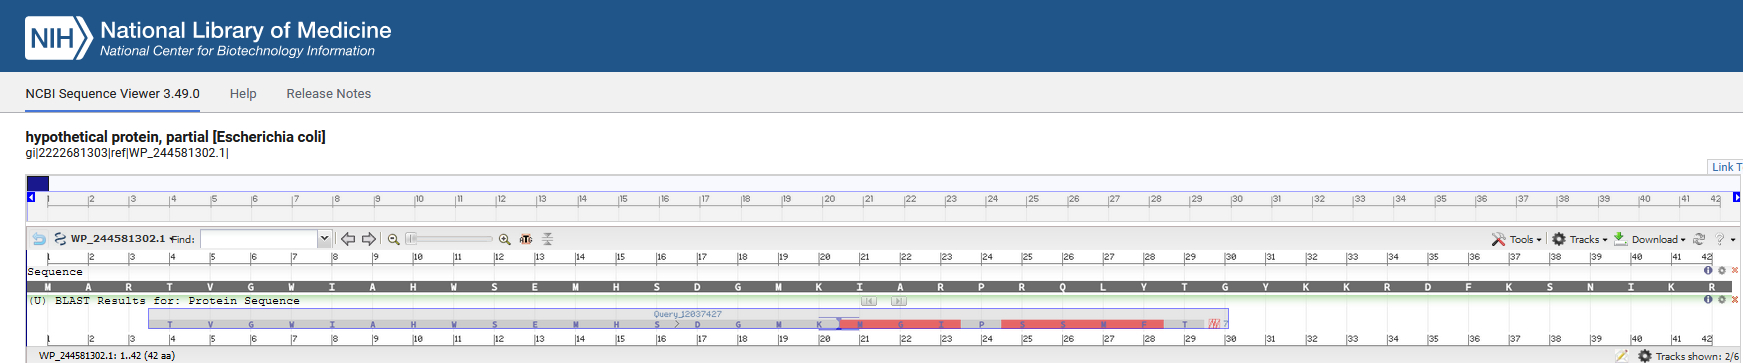
\includegraphics[width=0.99\linewidth]{Project 1/alignement.png}
    \caption{Sequences aligned}
    \label{fig:enter-label}
\end{figure}

h) BLAST is often used to reconstruct genomes or genes from shotgun sequences. However the same principle could be used to find a phone number in a phone book in order of likelihood if you start from a washed-away phone number on a napkin, or a teared/mistyped one. One could also use BLAST for Linguistic Studies, like finding which Languages use a certain word or variants of it.  \\

\chapter{Project 2}
This Project consists of finding various information on our protein of interest (2-methyl Citrate Synthase) from databases such as KEGG [\cite{kanehisa_kegg_2023}] and ExPASy [\cite{gasteiger_expasy_2003}].
\section{results}

\subsection{enzyme report from \textit{Uniprot}}
Uniprot is a database which provides general informations of proteins. Further introduction of uniprot is provided at 2.2.a. Some searching results of 2-Methyl citrate synthase(basic informations, names and taxonomy) obtained from uniprot is shown in figure 2.1 and 2.2.\\

\begin{figure}[H]
    \centering
    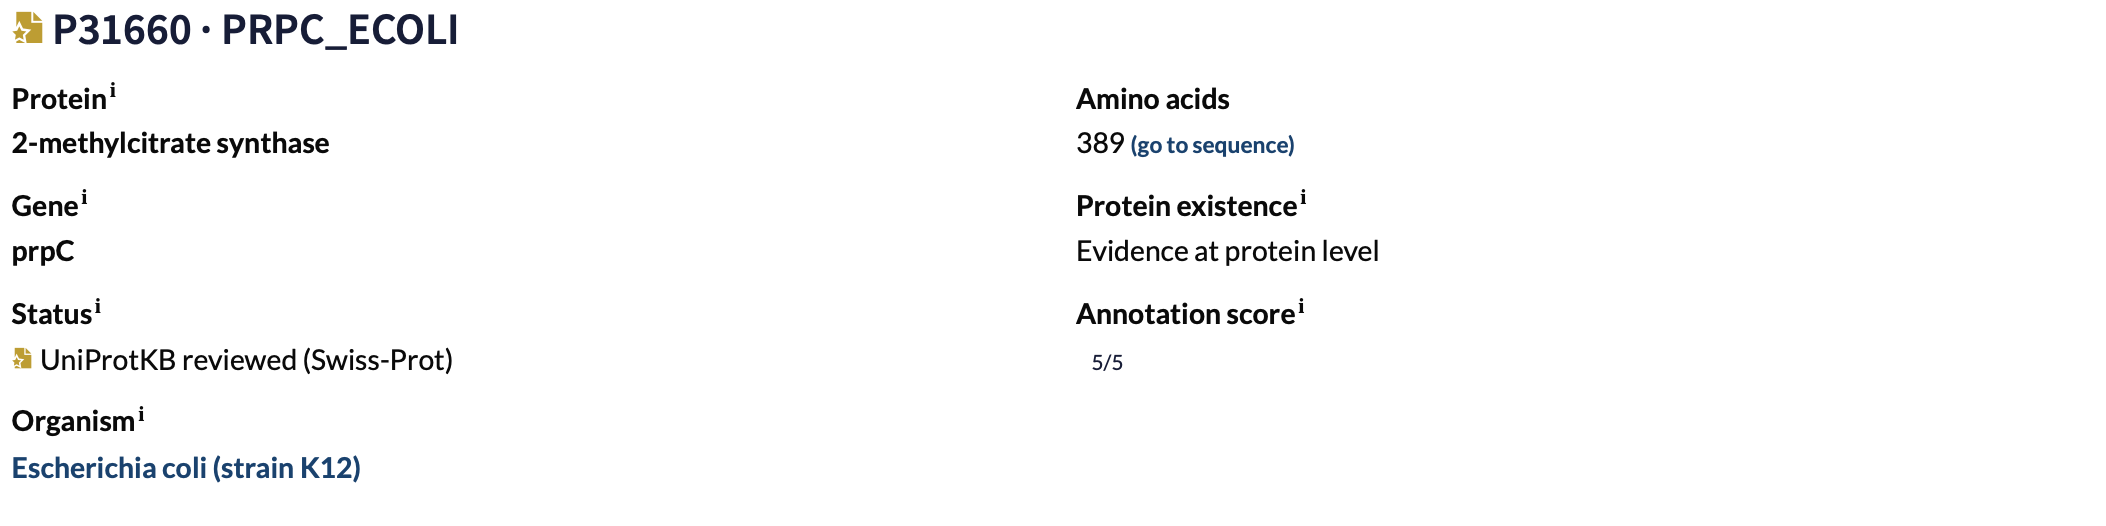
\includegraphics[width=0.9\linewidth]{Project 2/Uniprot images/Basic information.png}
    \caption{Uniprot code and basic informations of 2-Methyl citrate synthase}
\end{figure}

\begin{figure}[H]
    \centering
    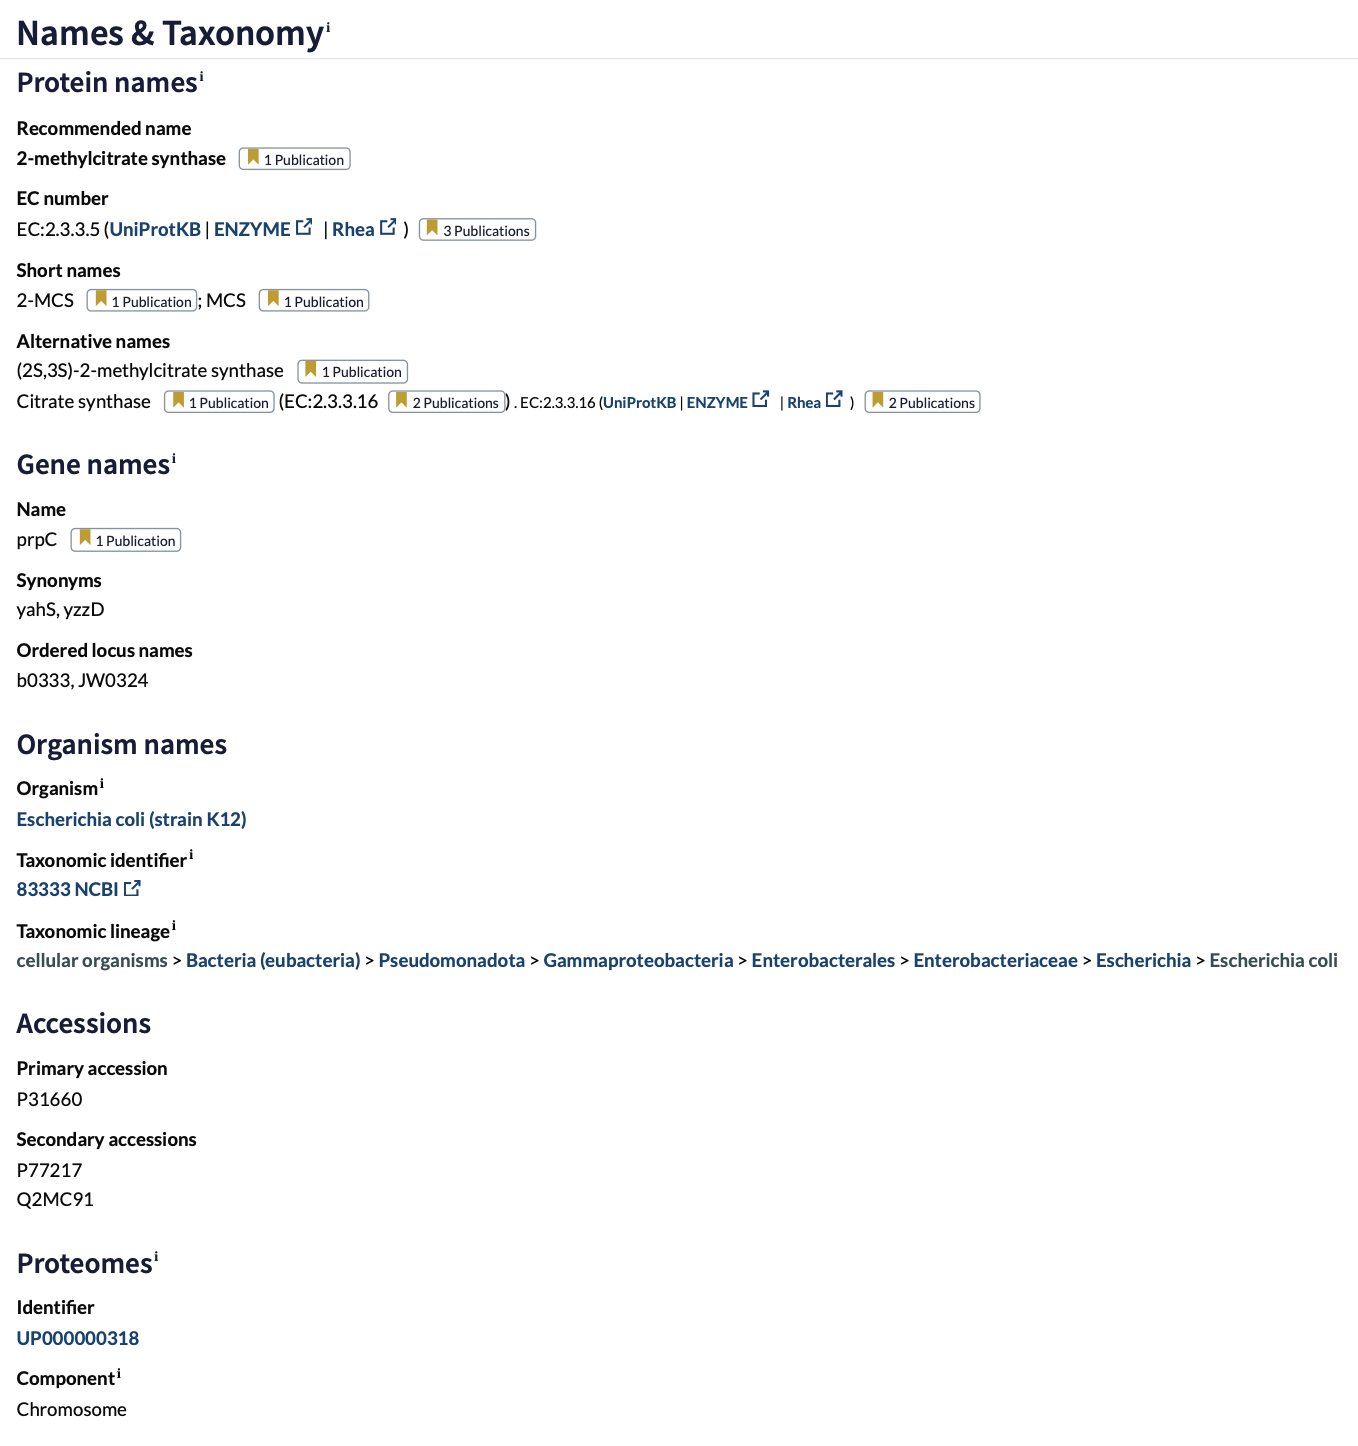
\includegraphics[width=0.9\linewidth]{Project 2/Uniprot images/Names and Taxonomy.png}
    \caption{Names and taxonomy of 2-Methyl citrate synthase}
\end{figure}

%the full sequence of the protein is here.

\subsection{Protein analysis using Rhea and String}

Except uniprot, there are some other databases, like Rhea[\cite{bansal_rhea_2022}] and STRING [\cite{szklarczyk_string_2021}], shows some specific properities of protein and enzymes. We obtained the chemical reaction catalysed by our enzyme via Rhea, and the interaction network of our enzyme from String.

\begin{figure}[H]
    \centering
    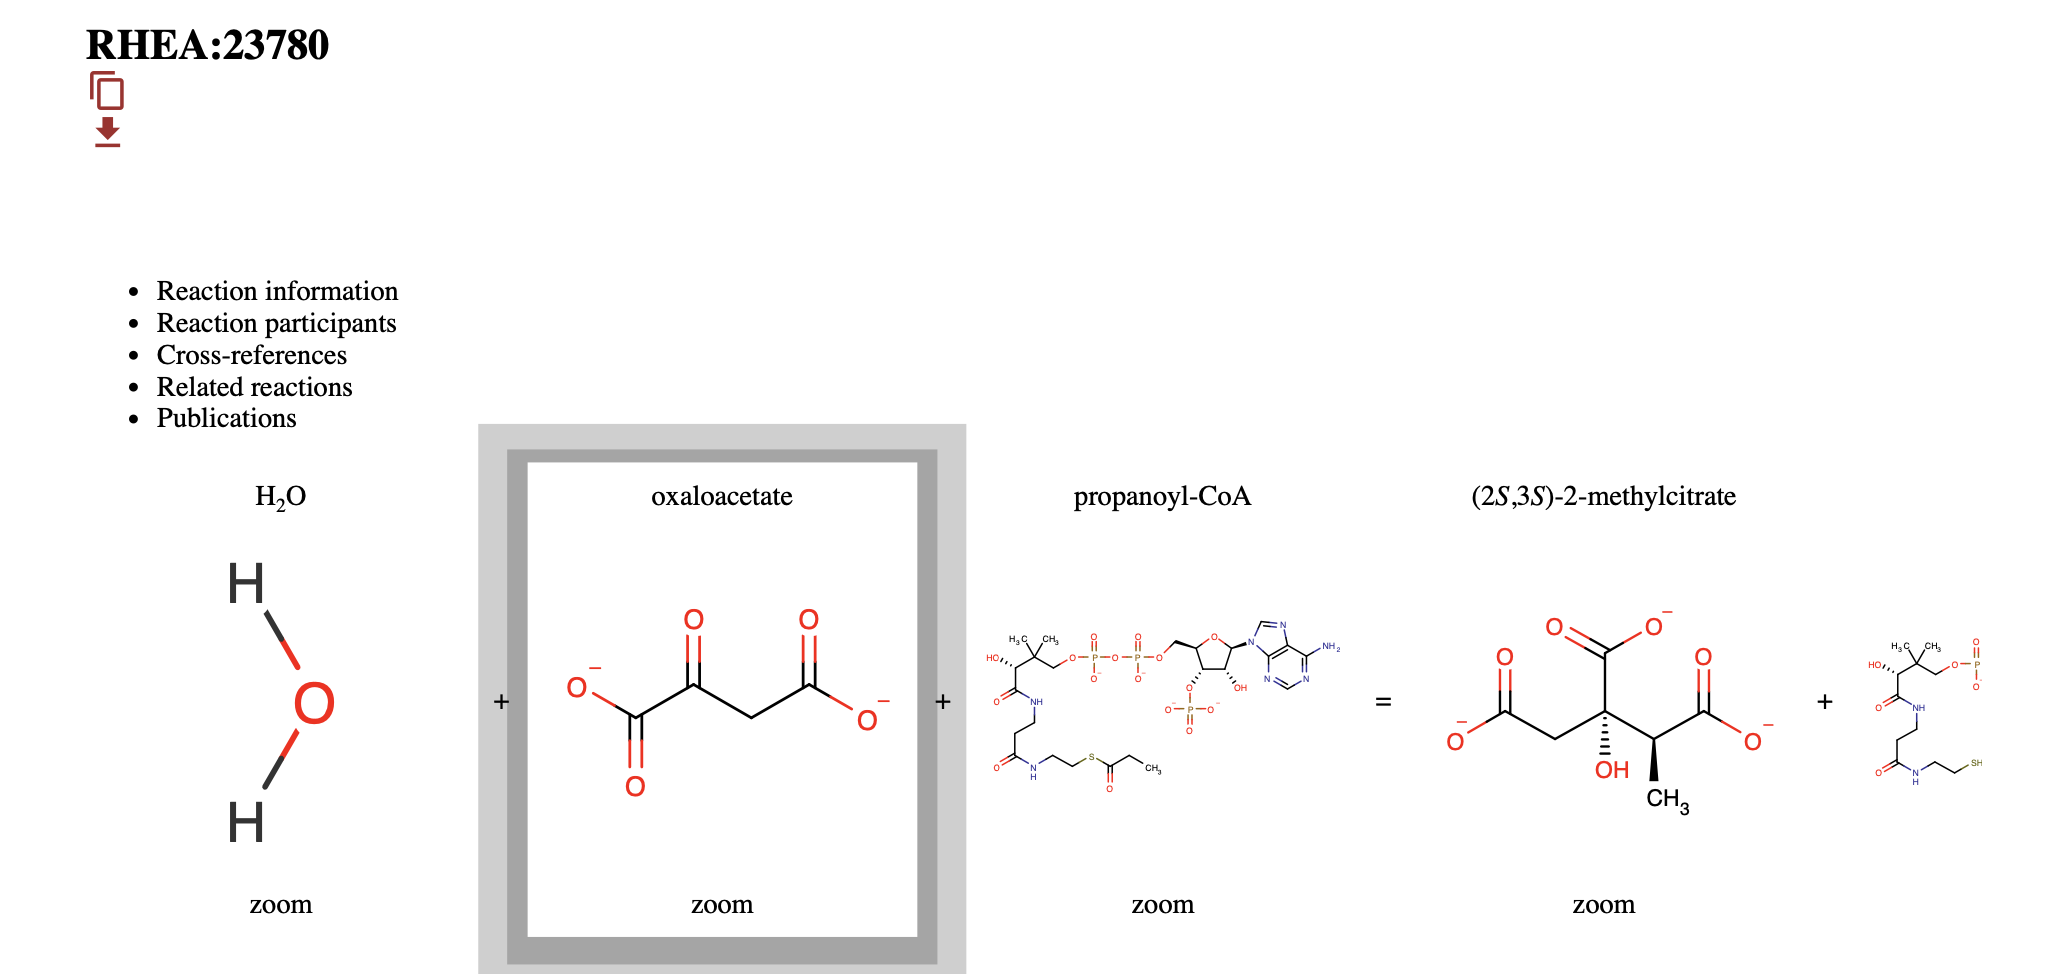
\includegraphics[width=0.9\linewidth]{Project 2/Images from Rhea and String/Rhea.png}
    \caption{The chemical reaction catalysed by 2-Methyl citrate synthase, acquired from Rhea}
\end{figure}


\begin{figure}[H]
    \centering
    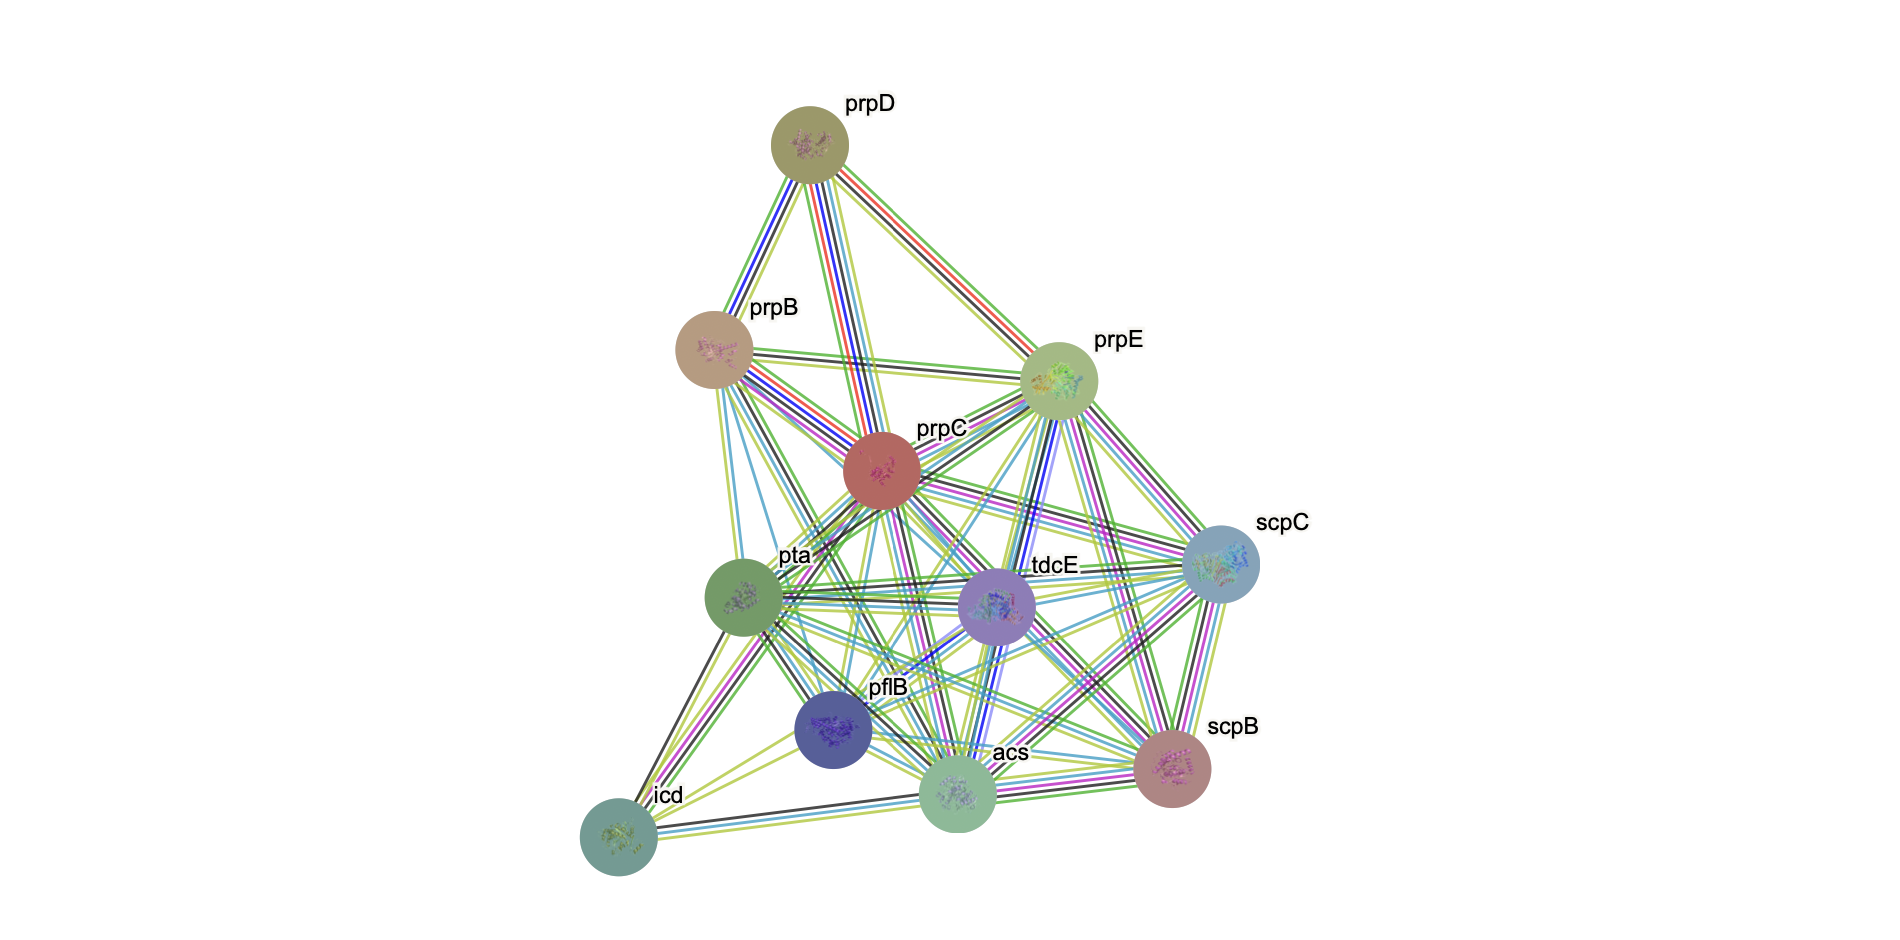
\includegraphics[width=0.9\linewidth]{Project 2/Images from Rhea and String/string 1.png}
    \caption{The interaction networks of 2-Methyl citrate synthase, acquired from String }
\end{figure}



\begin{figure}[H]
    \centering
    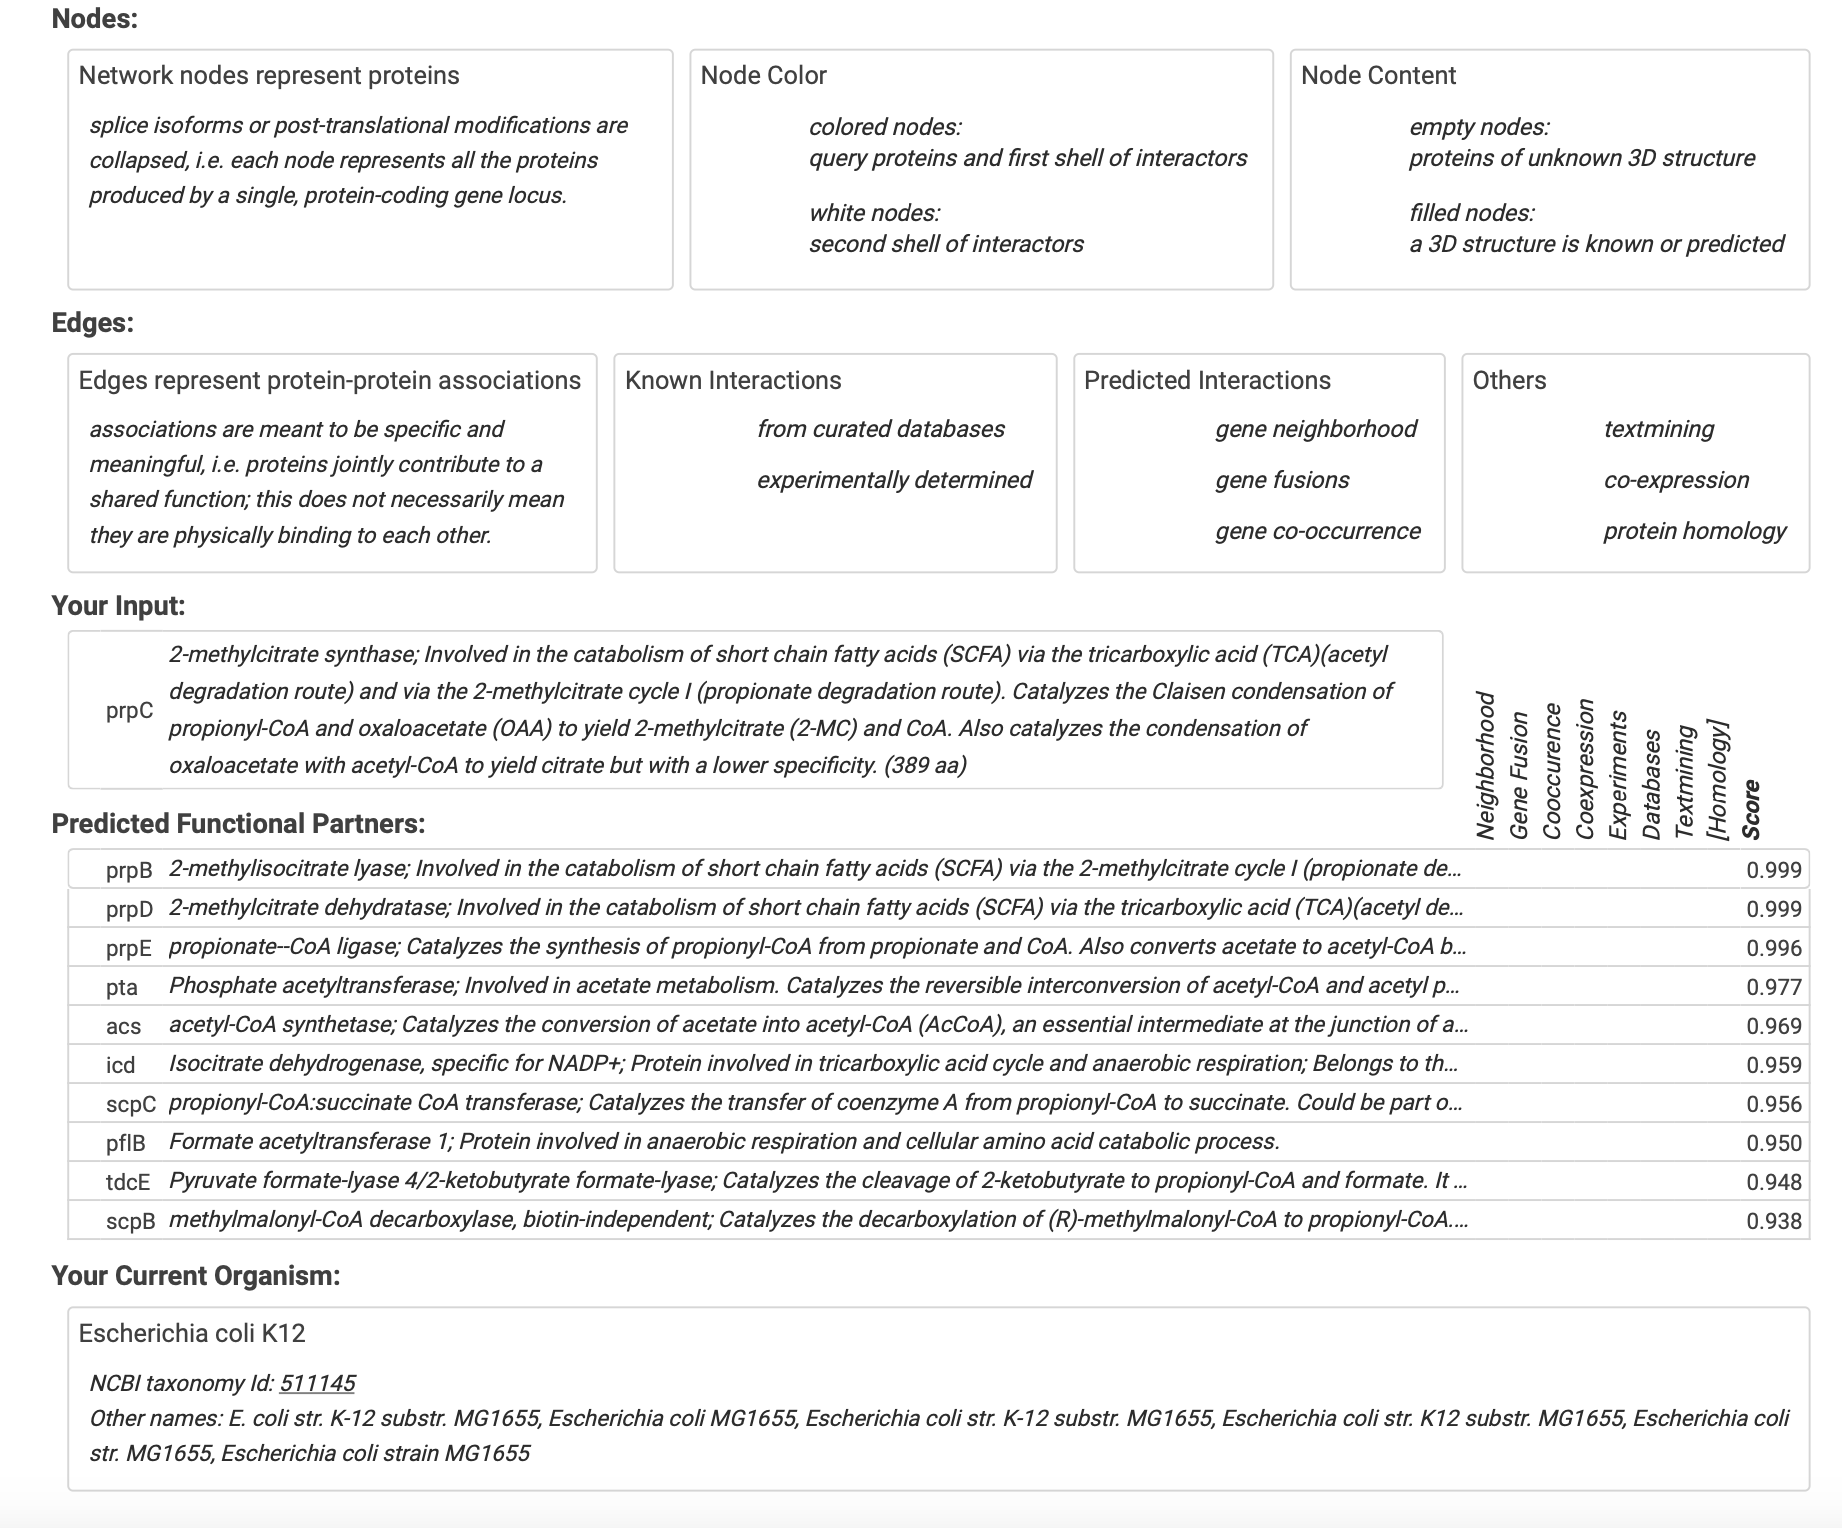
\includegraphics[width=0.9\linewidth]{Project 2/Images from Rhea and String/string 2.png}
    \caption{Explanations on the interaction network, acuiqred from String}
\end{figure}

\subsection{enzyme report from \textit{ENZYME}}
%Here would also contain the differences between enzyme and uniprot, why this pages doesn't have the sequence(Becaues they show a type of enzyme instead of one exact enzyme)
ENZYME database could be used to search for the enzyme type of the protein. In ENZYME database, we found the enzyme type of our protein. 2-Methyl cirtate synthase belongs to EC 2.3.3.5. 
\begin{figure}[H]
    \centering
    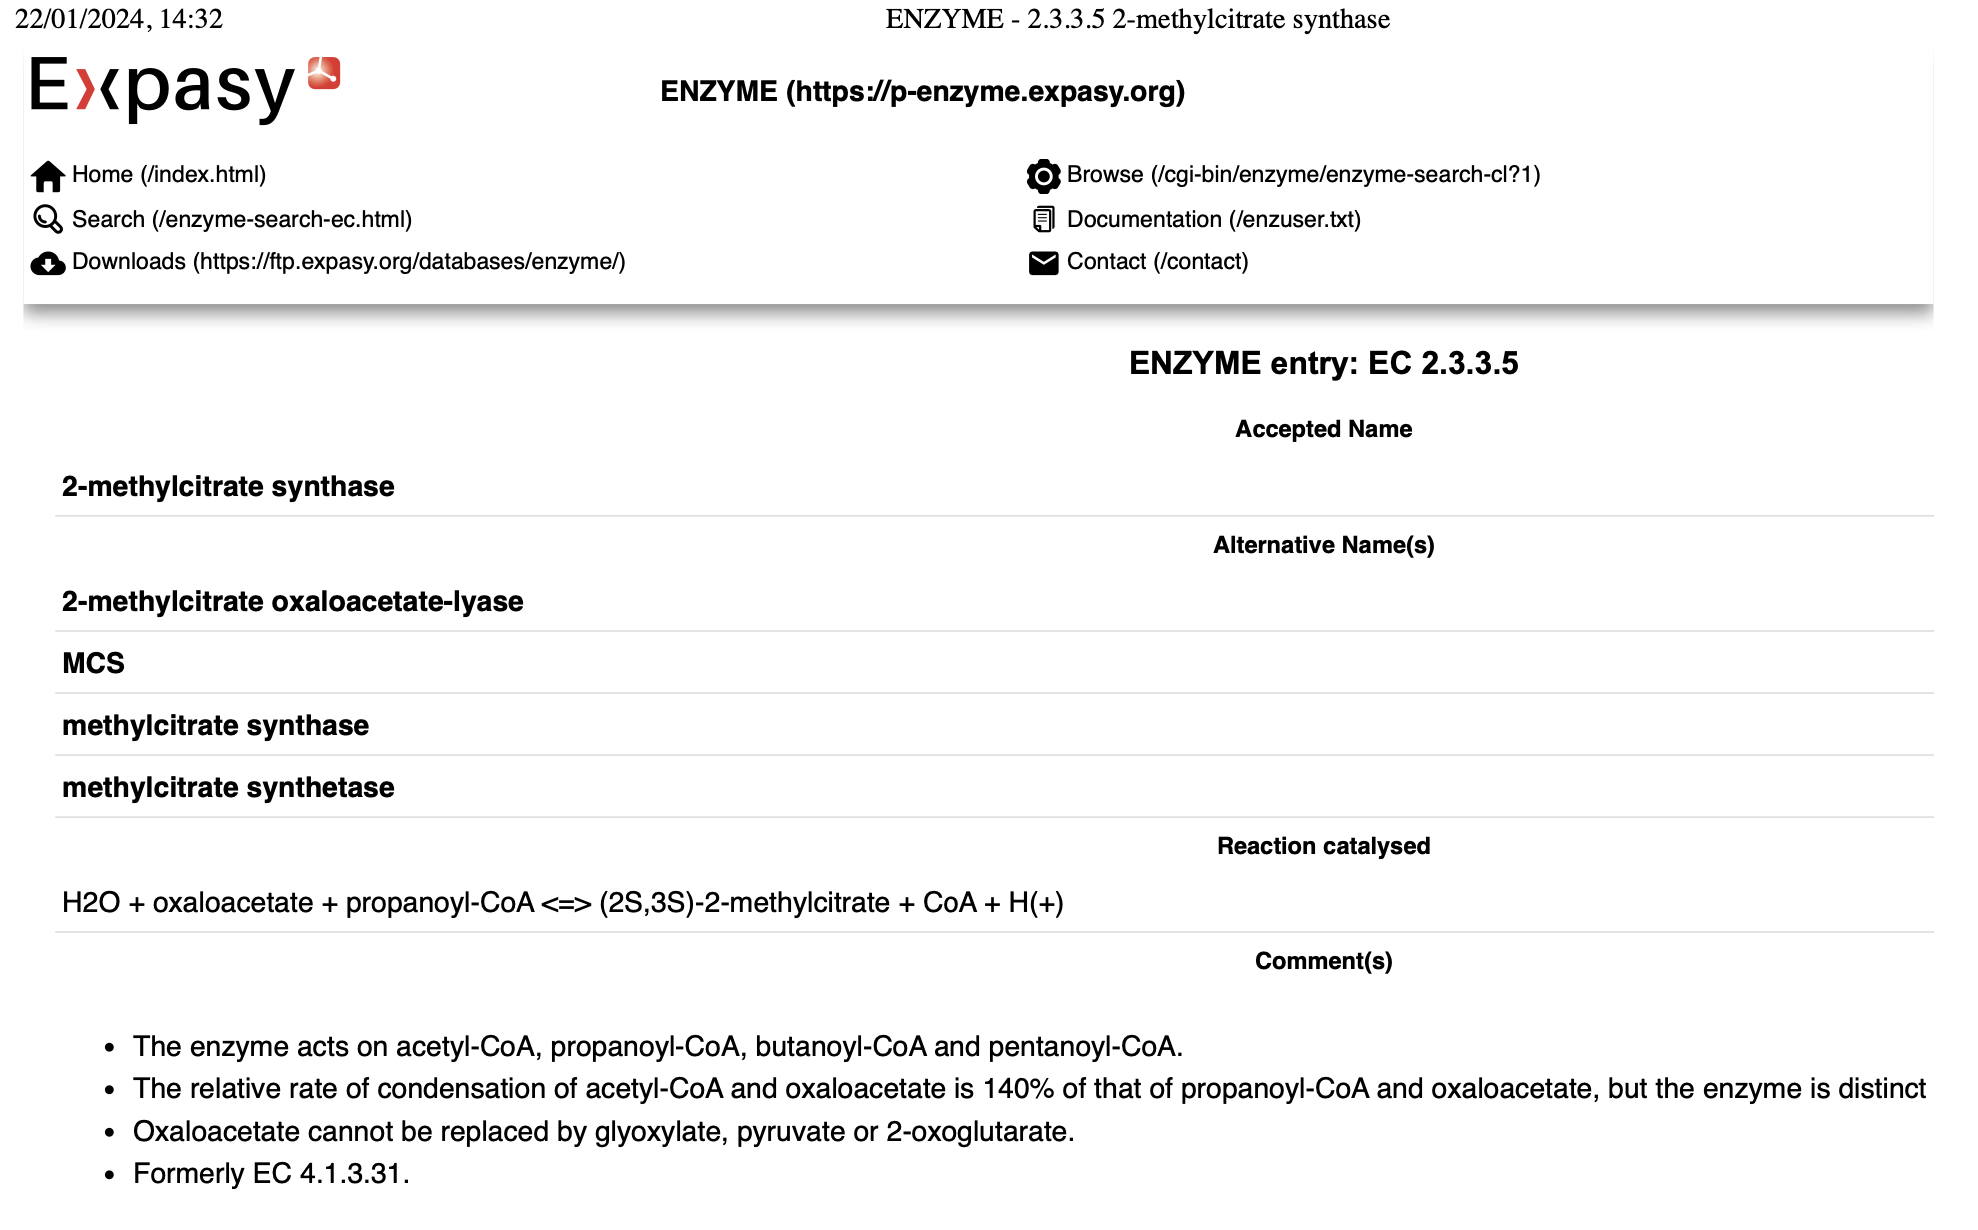
\includegraphics[width=0.9\linewidth]{Project 2/ENZYME images/Enzyme.png}
    \caption{The EC number and catalysed reaction of our protein}
\end{figure}

\subsection{KEGG pathways of 2-Methyl Citrate Synthase}
%It should contain the information of our enzyme, the circle representing the starting material(maybe we need a new image of it), and the Homo sapiens filtered results.
%question here: To what use could you put the knowledge taht metabolic pathways between two organisms sometimes differ?
In KEGG database [\cite{kanehisa_kegg_2023}], we obtained the (propanoate)metabolic pathways of EC 2.3.3.5. (figure 2.8 and 2.9). And then we looked at the metabolic pathways in homo sapines. As is shown in the figure 2.10 and 2.11, EC 2.3.3.5 does not involve in the reaction of homo sapines.

\begin{figure}[H]
    \centering
    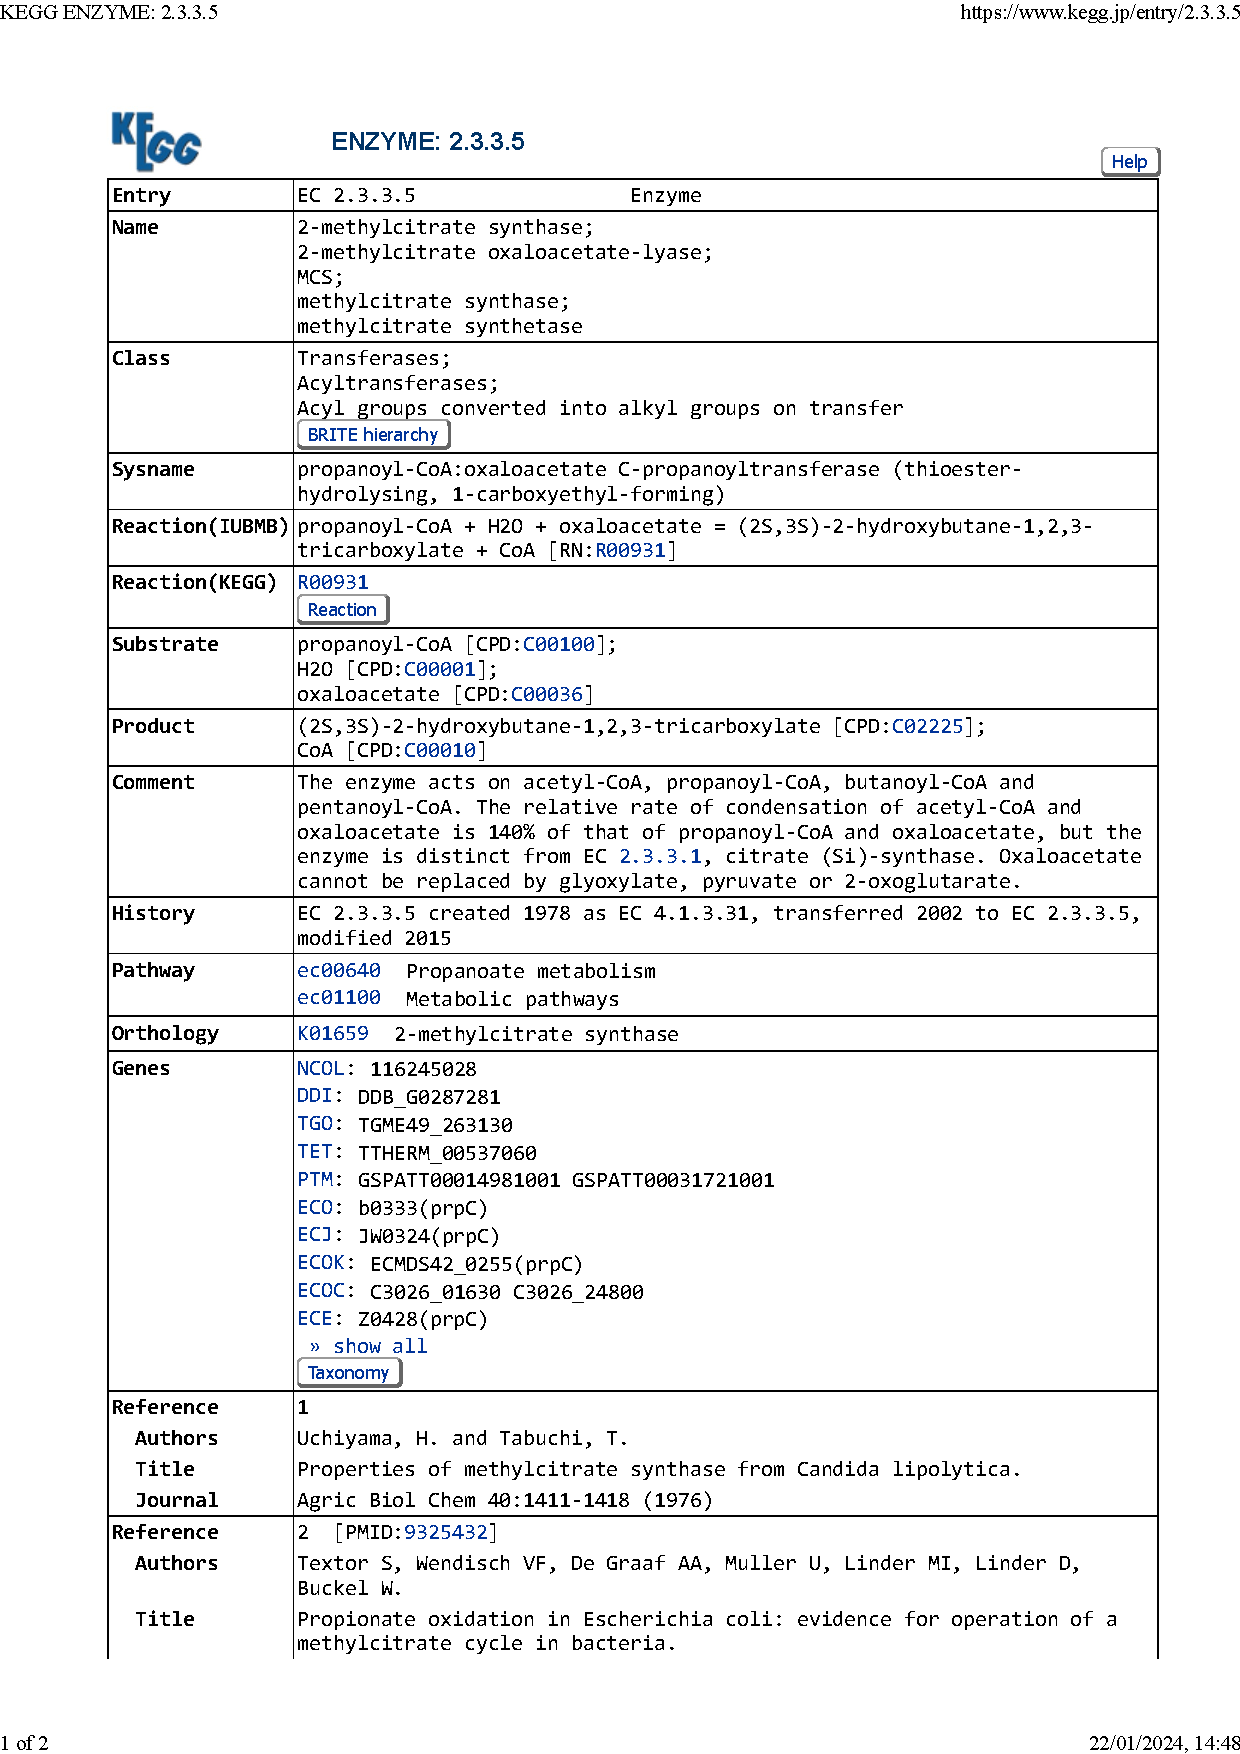
\includegraphics[width=0.9\linewidth]{Kegg 2-3-3-5 Hyperlink.pdf}
    \caption{The introduction on EC 2.3.3.5 generated from KEGG database}
\end{figure}

\begin{figure}[H]
    \centering
    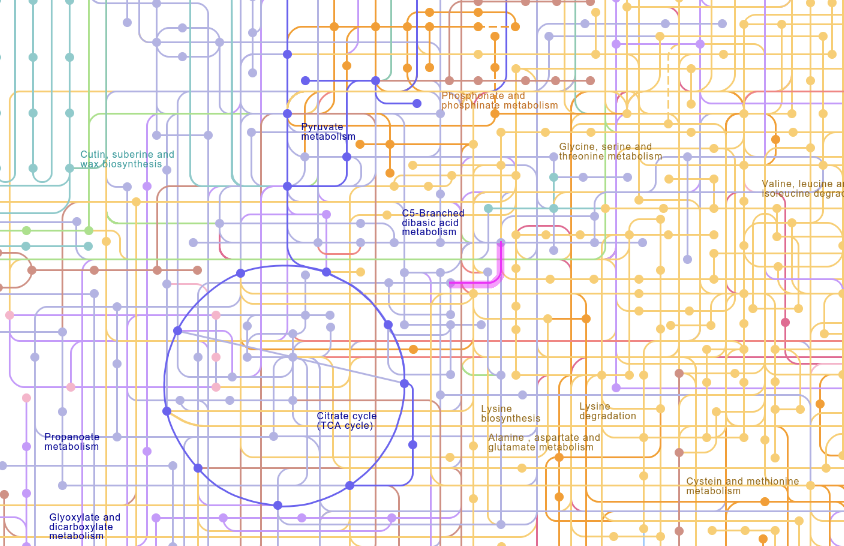
\includegraphics[width=0.9\linewidth]{Project 2/Kegg pathways/metabolic pathways.png}
    \caption{Part of the metabolic pathways, the pink sparkling pathway is related to EC 2.3.3.5}
\end{figure}

\begin{figure}[H]
    \centering
    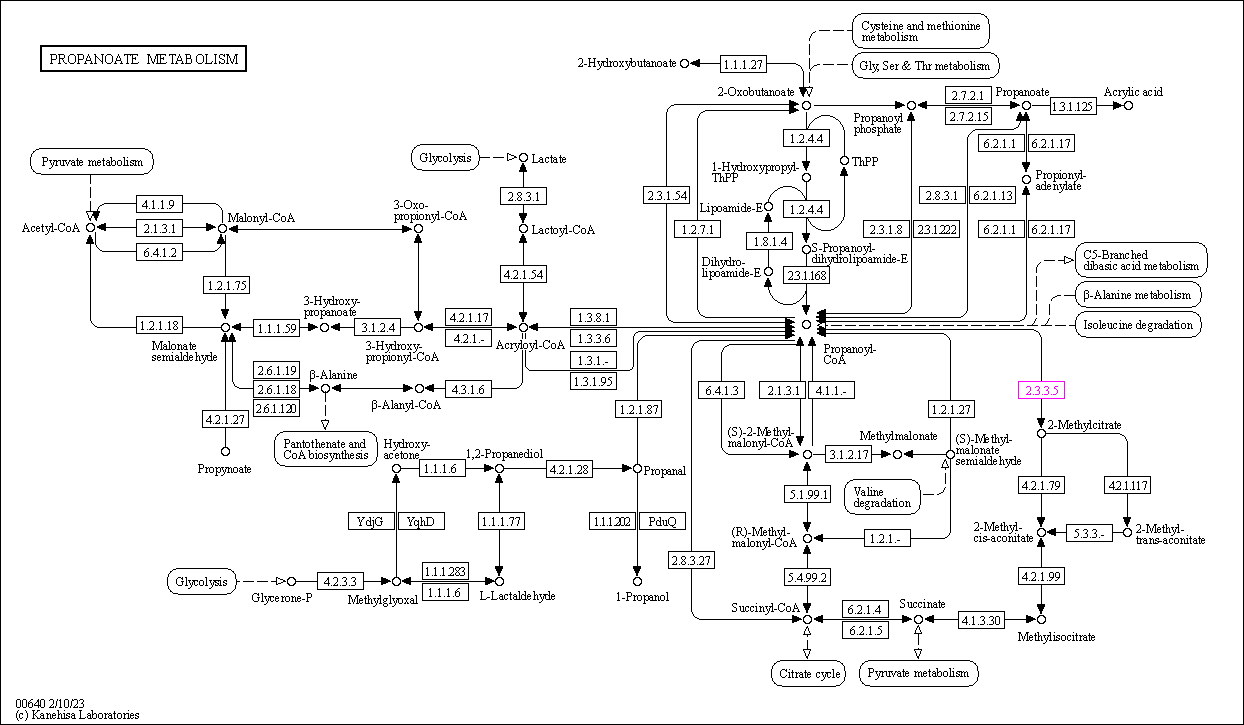
\includegraphics[width=0.9\linewidth]{Project 2/Kegg pathways/Propanoate metabolism.png}
    \caption{The propanoate metabolic pathways, the red part is related to EC 2.3.3.5}
\end{figure}

\begin{figure}[H]
    \centering
    
\includegraphics[width=0.9\linewidth]{Project 2/Kegg pathways/metabolic pathways hs.png}
    \caption{Part of the metabolic pathways in homo sapines. The green pathways are the pathways exist in homo sapines.}
\end{figure}

\begin{figure}[H]
    \centering
    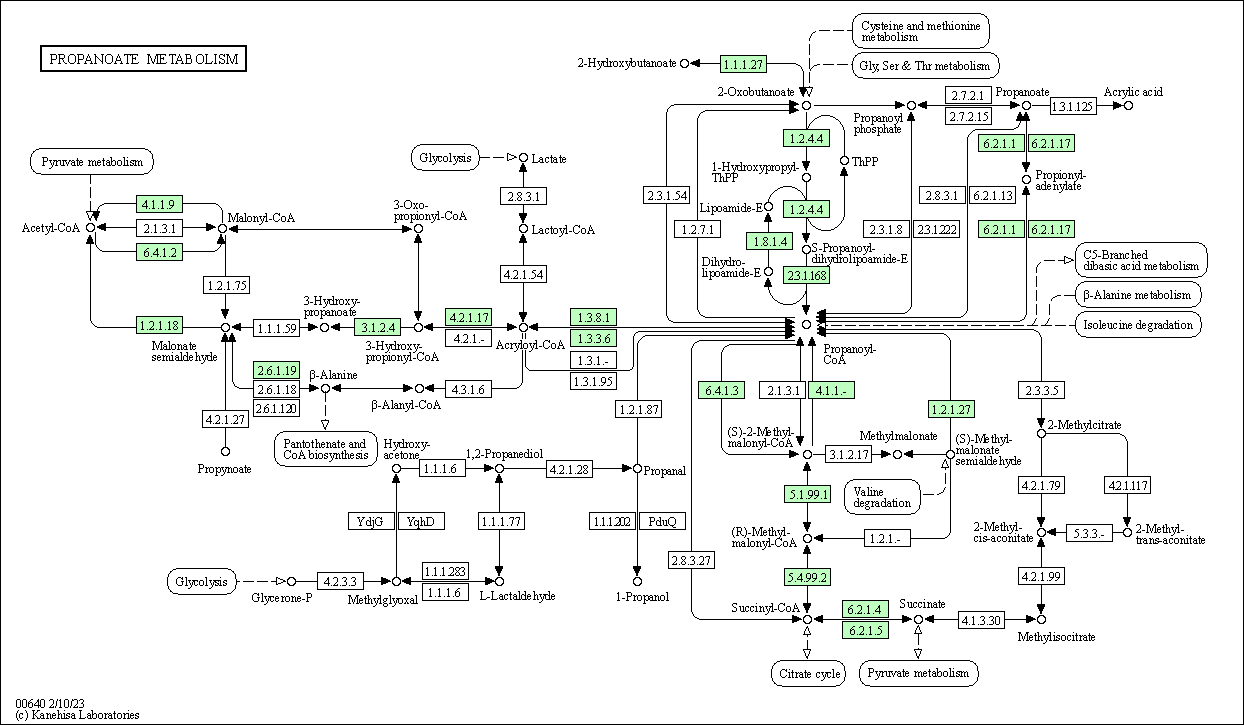
\includegraphics[width=0.9\linewidth]{Project 2/Kegg pathways/propanoate metabolism in hs.png}
    \caption{The propanoate metabolic pathways in homo sapines. The green pathways are the pathways exist in homo sapines}
\end{figure}

\subsection{Gene defect analysis using OMIM database}
%Show that if there are some genetic defects(No it doesn't even in the human body,)
The information of 2-Methyl Citrate Synthase does not exist in the OMIM database. 
\section{discussions}

a) Uniprot gives general-purpose information on the protein, it specifies various aspects like: Cell localization, names and taxonomy, expression, interaction,  sequence, relative PDB entries or alphafold-predicted structure. UniProt allows us to have an "Omic" view of the protein. Whereas ENZYME focuses on the enzymatic activity, from a chemical perspective of reactions, products, conditions of temperature and pH. It also provides all the publications and resources relative to claims.

b) The following figure is the cleavage maps of our protein sequence( corresponding to the UniProt entry P31660 ), the cleavage was performed by Trypsin, High-affinity Chymotrypsin, and Cyanogen-Bromide.
The maps allow us to simply visualize where the cut sites are concentrated, and if any sites are cleaved by more than one enzyme.
These maps were computed trough the use of Expasy - Peptide Cutter [\cite{PeptideProerty}]

\begin{figure}[H]
    \centering
    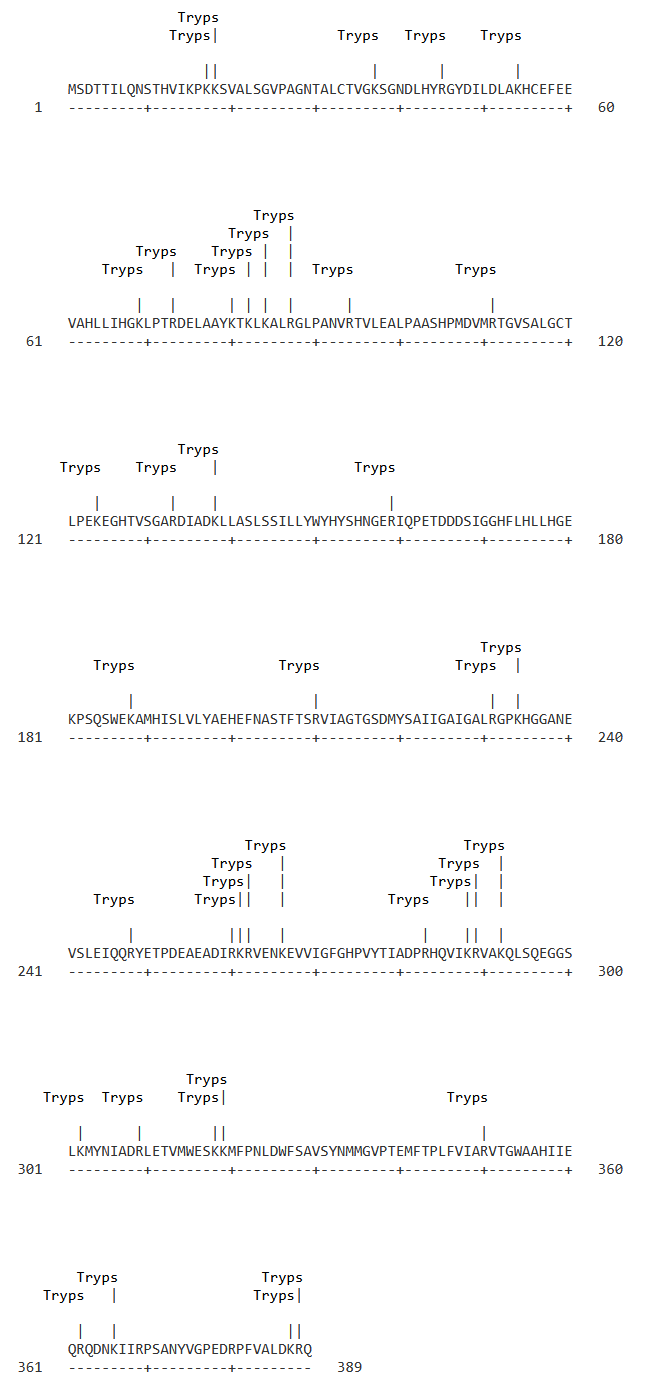
\includegraphics[width=0.3\linewidth]{Project 2/trypsin.png}
    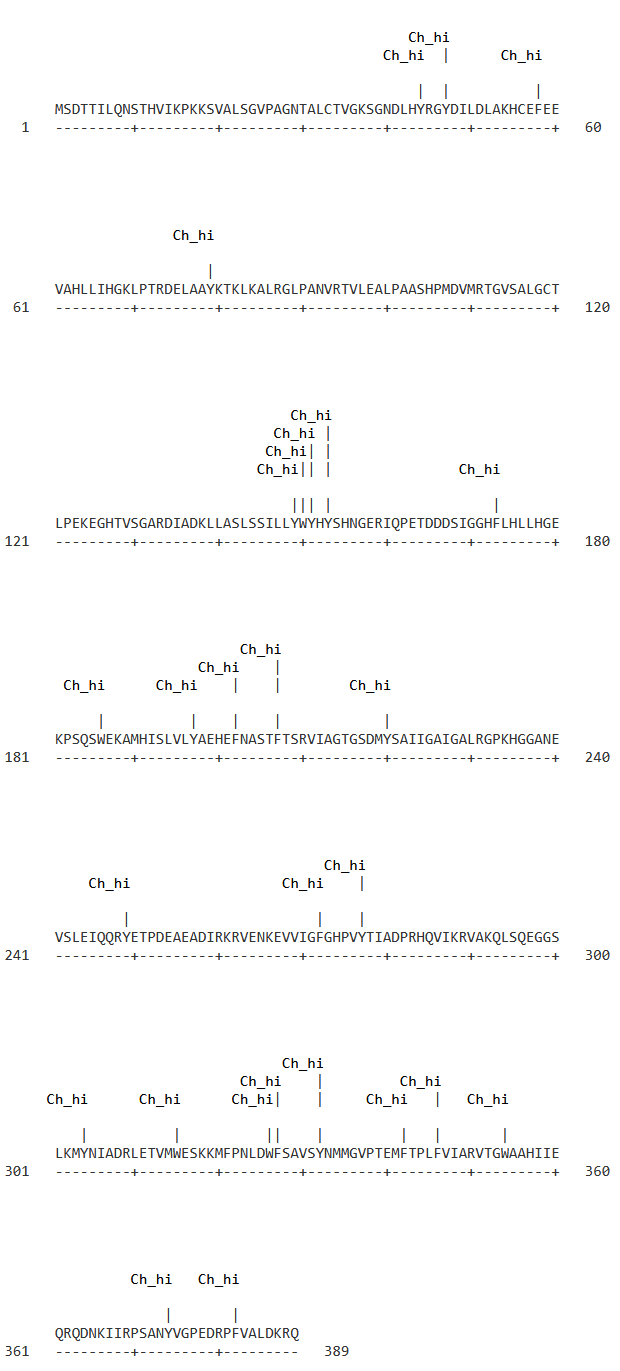
\includegraphics[width=0.3\linewidth]{Project 2/Hymotrypsin.png}
    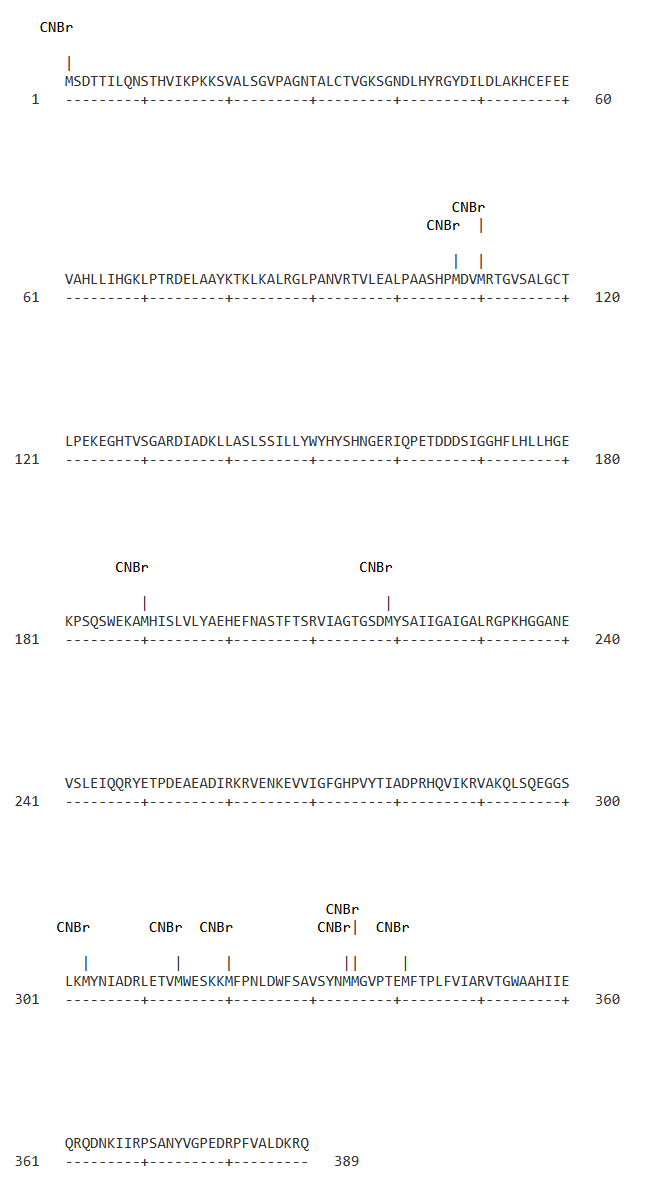
\includegraphics[width=0.3\linewidth]{Project 2/CyanogenBromide.png}
    \caption{Cleavage Sites of trypsin Hi-Aff. chymotrypsin and CyanogenBromide}
\end{figure}

In the following table we can see the peptide sequence of one of the resulting peptides after enzymatic digestion with trypsin, we also have the molecular weight and Net-charge values at different pH Levels.
\begin{table}[H]
\centering
\begin{tabular}{|l|l|}
\hline
\textbf{Peptide Sequence} & MSDTTILQNSTHVIKPK \\
\hline
\textbf{Molar Weight} & 1913.19 g/mol \\
\hline
\textbf{Peptide Net-Charge pH2} & 3.7 \\
\hline
\textbf{Peptide Net-Charge pH7} & 1.1 \\
\hline
\textbf{Peptide Net-Charge pH9} & 0.8 \\
\hline
\end{tabular}
\caption{Peptide Calculations}
\end{table}

The following figure displays a continuous plot of the Net-charge over all pH values.
\begin{figure}[H]
    \centering
    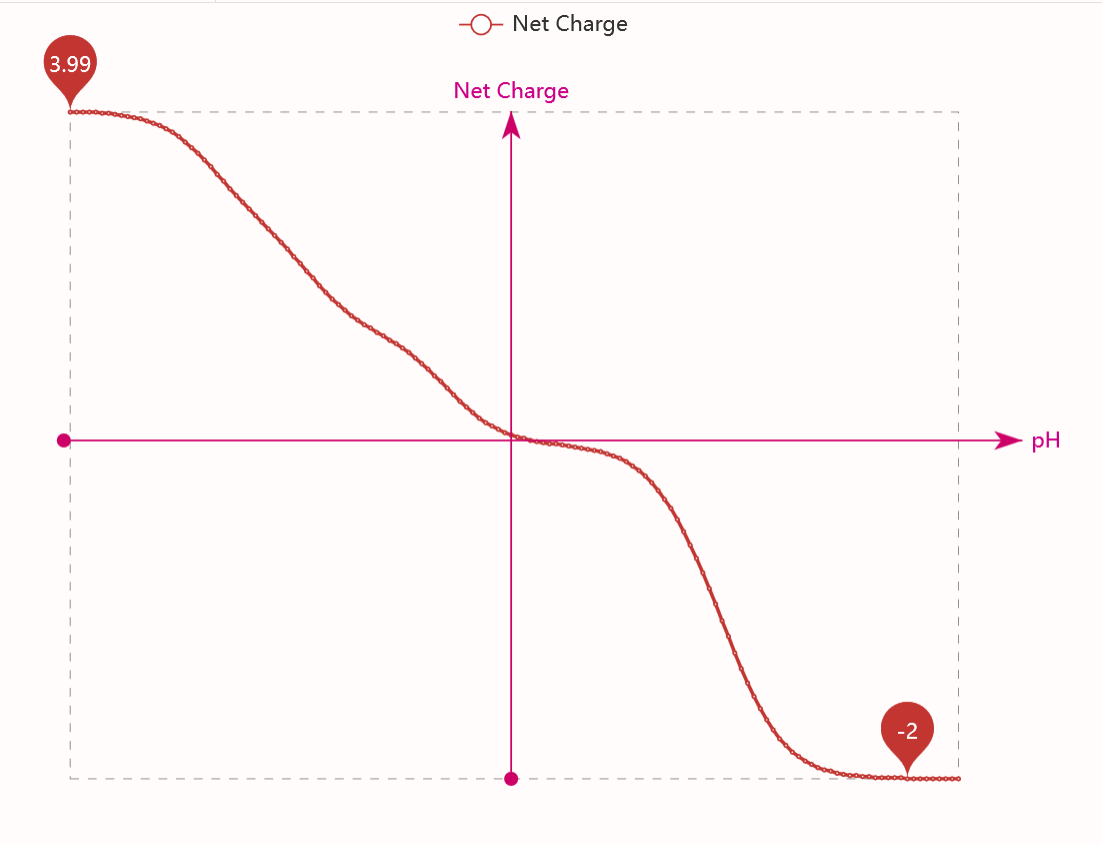
\includegraphics[width=0.50\linewidth]{Project 2/Netcharge.png}
    \caption{Net-charge plot of 2-methylcitrate synthase }
\end{figure}

c) It is involved in the catabolism of short chain fatty acids (SCFA) via the tricarboxylic acid (TCA)(acetyl degradation route) and via the 2-methylcitrate cycle I (propionate degradation route). Catalyzes the Claisen condensation of propionyl-CoA and oxaloacetate (OAA) to yield 2-methylcitrate (2-MC) and CoA. Also catalyzes the condensation of oxaloacetate with acetyl-CoA to yield citrate but with a lower specificity.

d) The enzyme we investigated requires coenzyme A as a cofactor.

e) 2-methylcitrate synthase catalyzes the conversion of propionyl-CoA and oxaloacetate into 2-methylcitrate by allowing the transfer of an acyl group which is converted into an alkyl upon transfer. This reaction is a crucial step in the anabolism of propionate, and thus energetic metabolism.

f) Our enzyme is associated with E. Coli, and more generally with bacteria, so a pathological study to see how a mutation affects the protein function , and therefore the organism as a whole, is beyond any reasonable scope, for this reason we assume there are no notable mutations associated with the protein.

\chapter{Project 3}


\begin{comment}
    

It's fine. How are you? Have you recovered from the sick?
Oh perfect! That's sounds great!
Glad to hear that! I'll go on with the report, 
Okay! Let's go:)

Hello Haiyang!! I am doing the stuff with pymol
how are you today? I am sorry for not doing anything these days...
:)
SAME!! I went with my bycicle to blaustein.
Yeah yeah, much better
Alright, I will do the same, Yes we can definetly finsh it by monday
good luck :)
\end{comment}

\section{results}
In the following section we will display the results relative to the three exercises required to better understand our protein from a structural perspective.
\subsection{Space filling vs Cartoons}

In figure 3.1 we can see representative views of the crystal structure of 2-methylcitrate synthase from Salmonella typhimurium, cultured in E.Coli.
On the left we can see a cartoon view displaying in cyan the alpha-helices, in red the antiparallel beta-sheet and in magenta the unstructured coils.
This type of depiction allows us to understand the protein from mechanic point of view, alpha-helices are very rigid structures that give the overall protein stability in holding it´s shape, it also allows to easily if the beta-sheets are parallel on antiparallel, and finally to visualize the number of inherently disordered regions which can be used for multiple purposes, like ubiquitination or protein transport.
On the right we can see a spacefill representation where the surface of the protein in  approximated, this type of view allows to better understand the topology of our protein and inspect if there are any pockets where solvents, ions or ligands could be held.
In fact we can recognize 3 aminoacids in yellow in what could be recognized as the enzymatic cleft.
\begin{figure}[H]
        \centering
        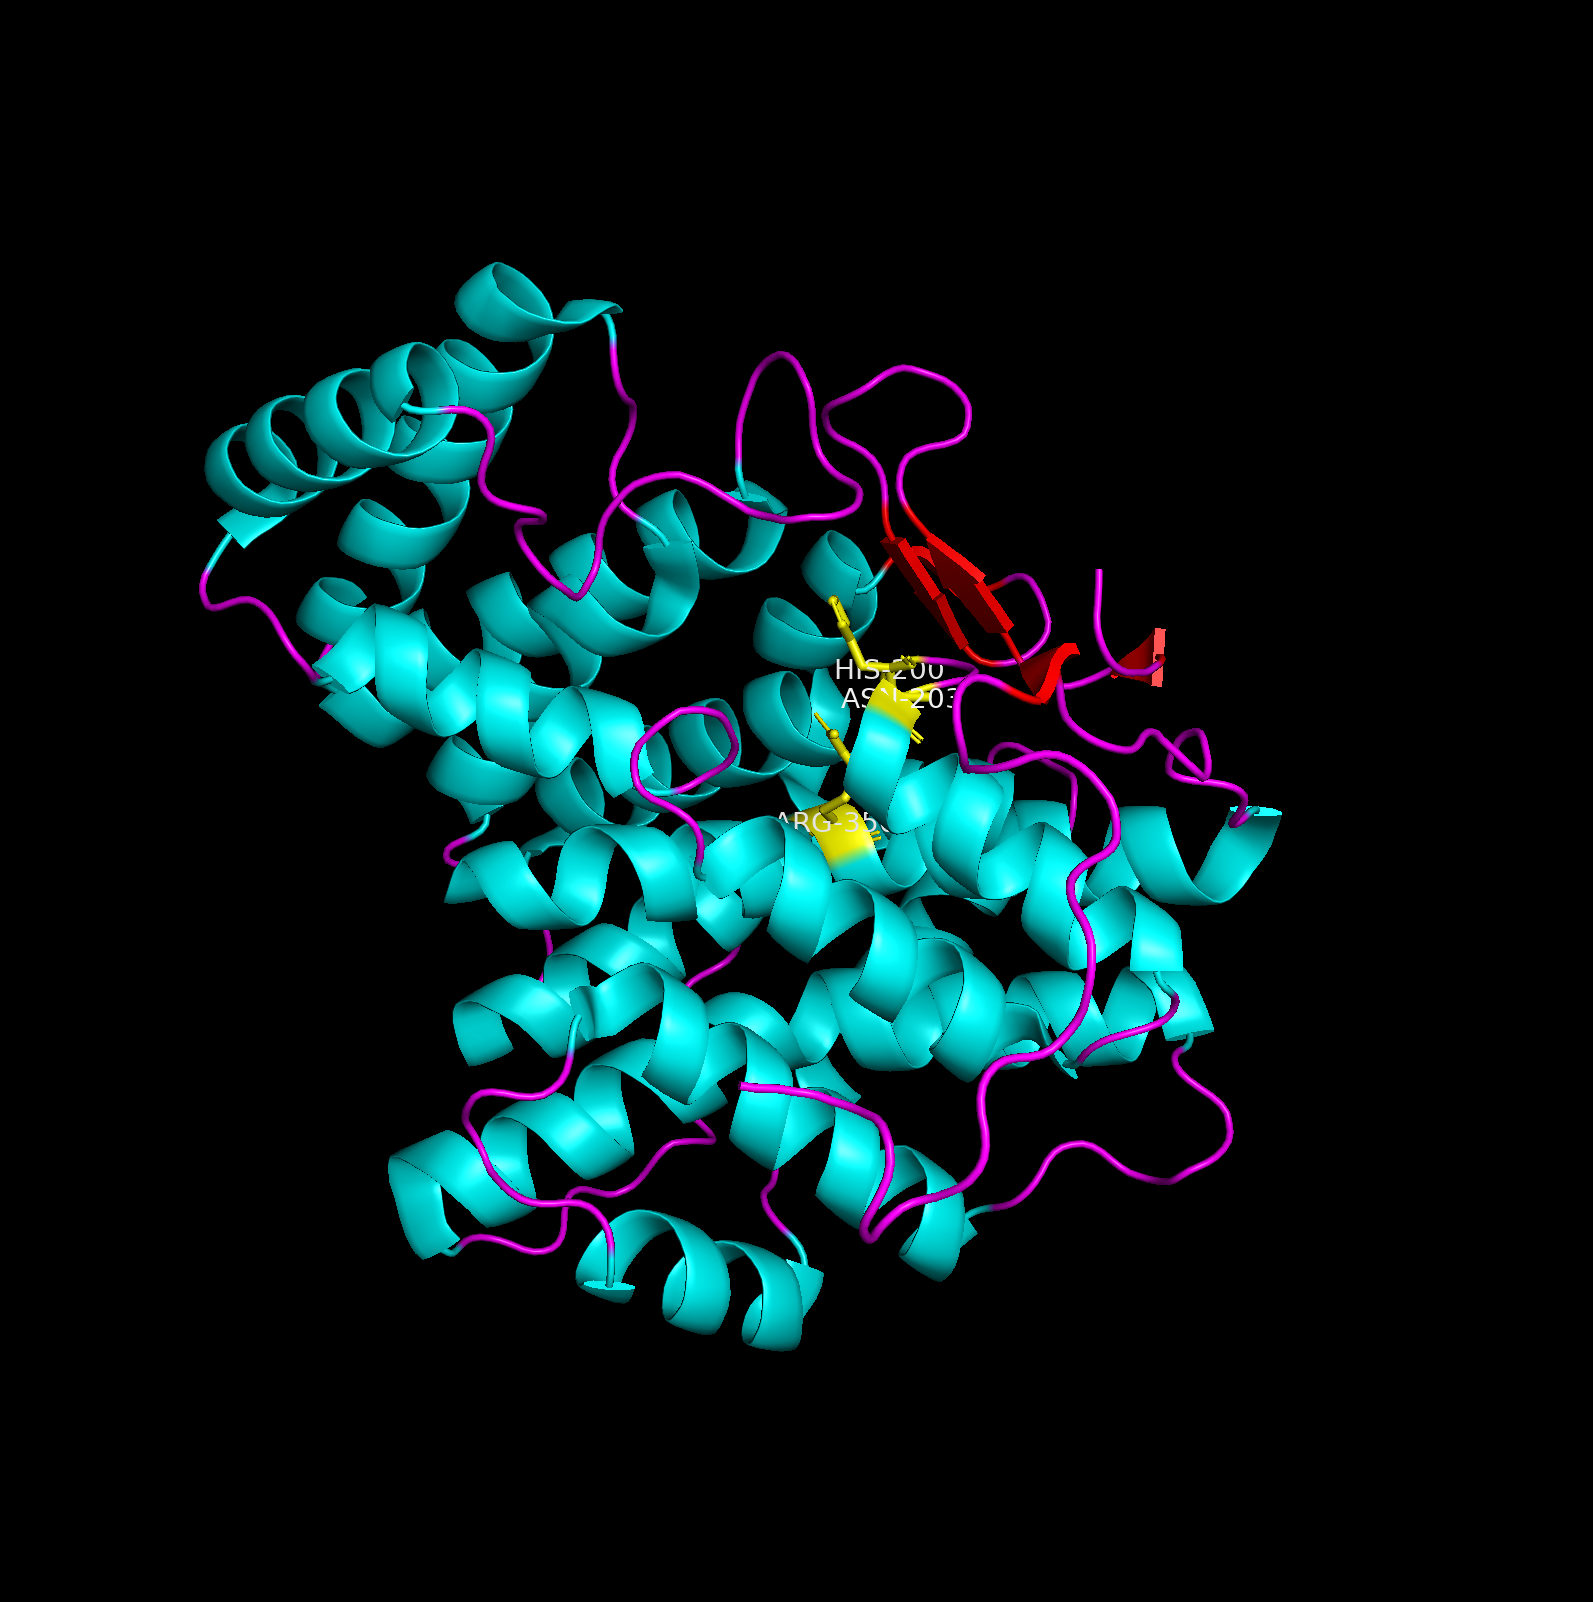
\includegraphics[width=0.45\textwidth]{Project 3/cartoonnew.png}
        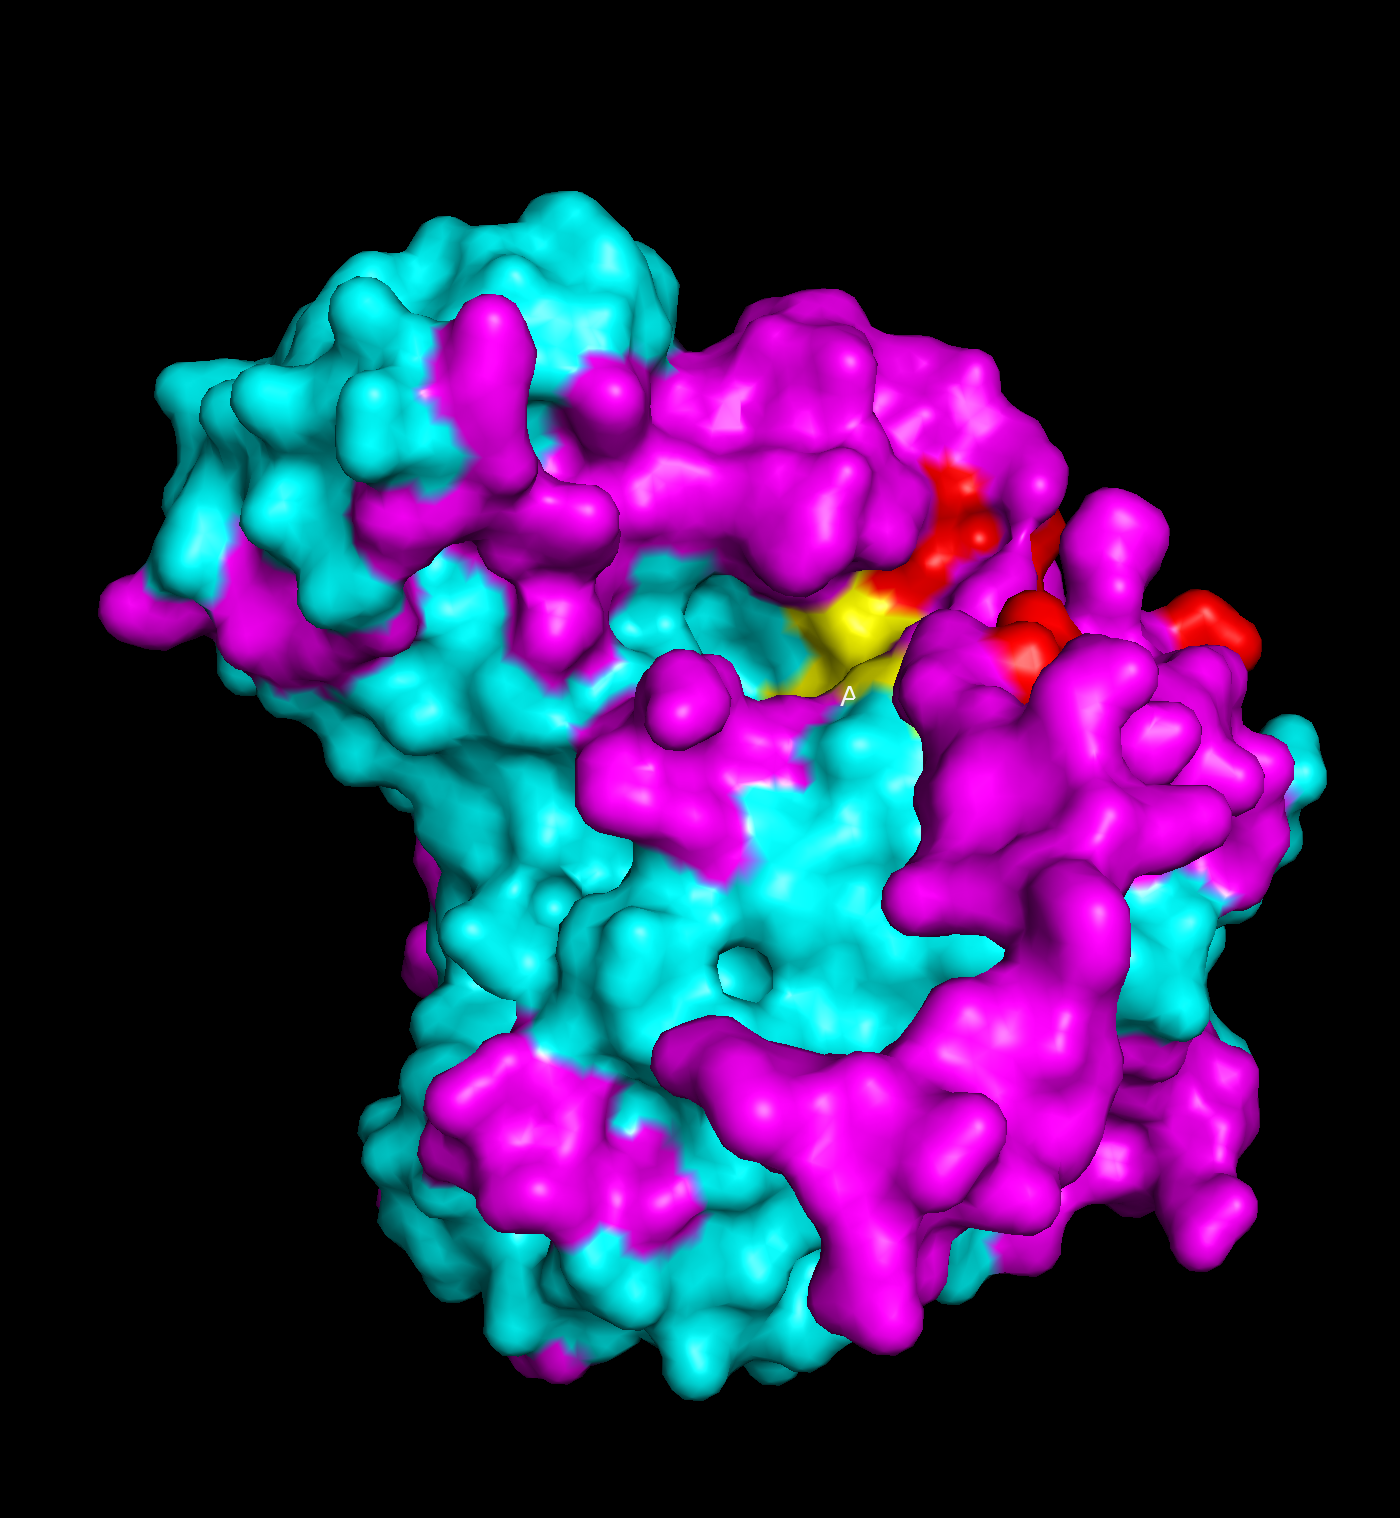
\includegraphics[width=0.42\textwidth]{Project 3/surfacenew.png}
	    \caption{Cartoon and Space-fill Representations. }
\end{figure}

\subsection{Enzymatic Pocket}
In Figure 3.2 we can see the enzymatic cleft of our protein around the Glycerol, and we can recognize that the Glycerol has dipole interactions with one water molecule and three distinct aminoacids, in particular Histidine-200, Arginine-350 and Asparagine-203.
Particular attention should be given to the role of the R group of Asparigine-203 in the enzymatic reaction, because it is the last aminaocid and it doesn´t contribute to the reaction with only the dipole moment of the aminoacid itself, but instead with the one created by the whole alpha-loop[\cite{hol_-helix_1978}].

\begin{figure}[H]
        \centering
        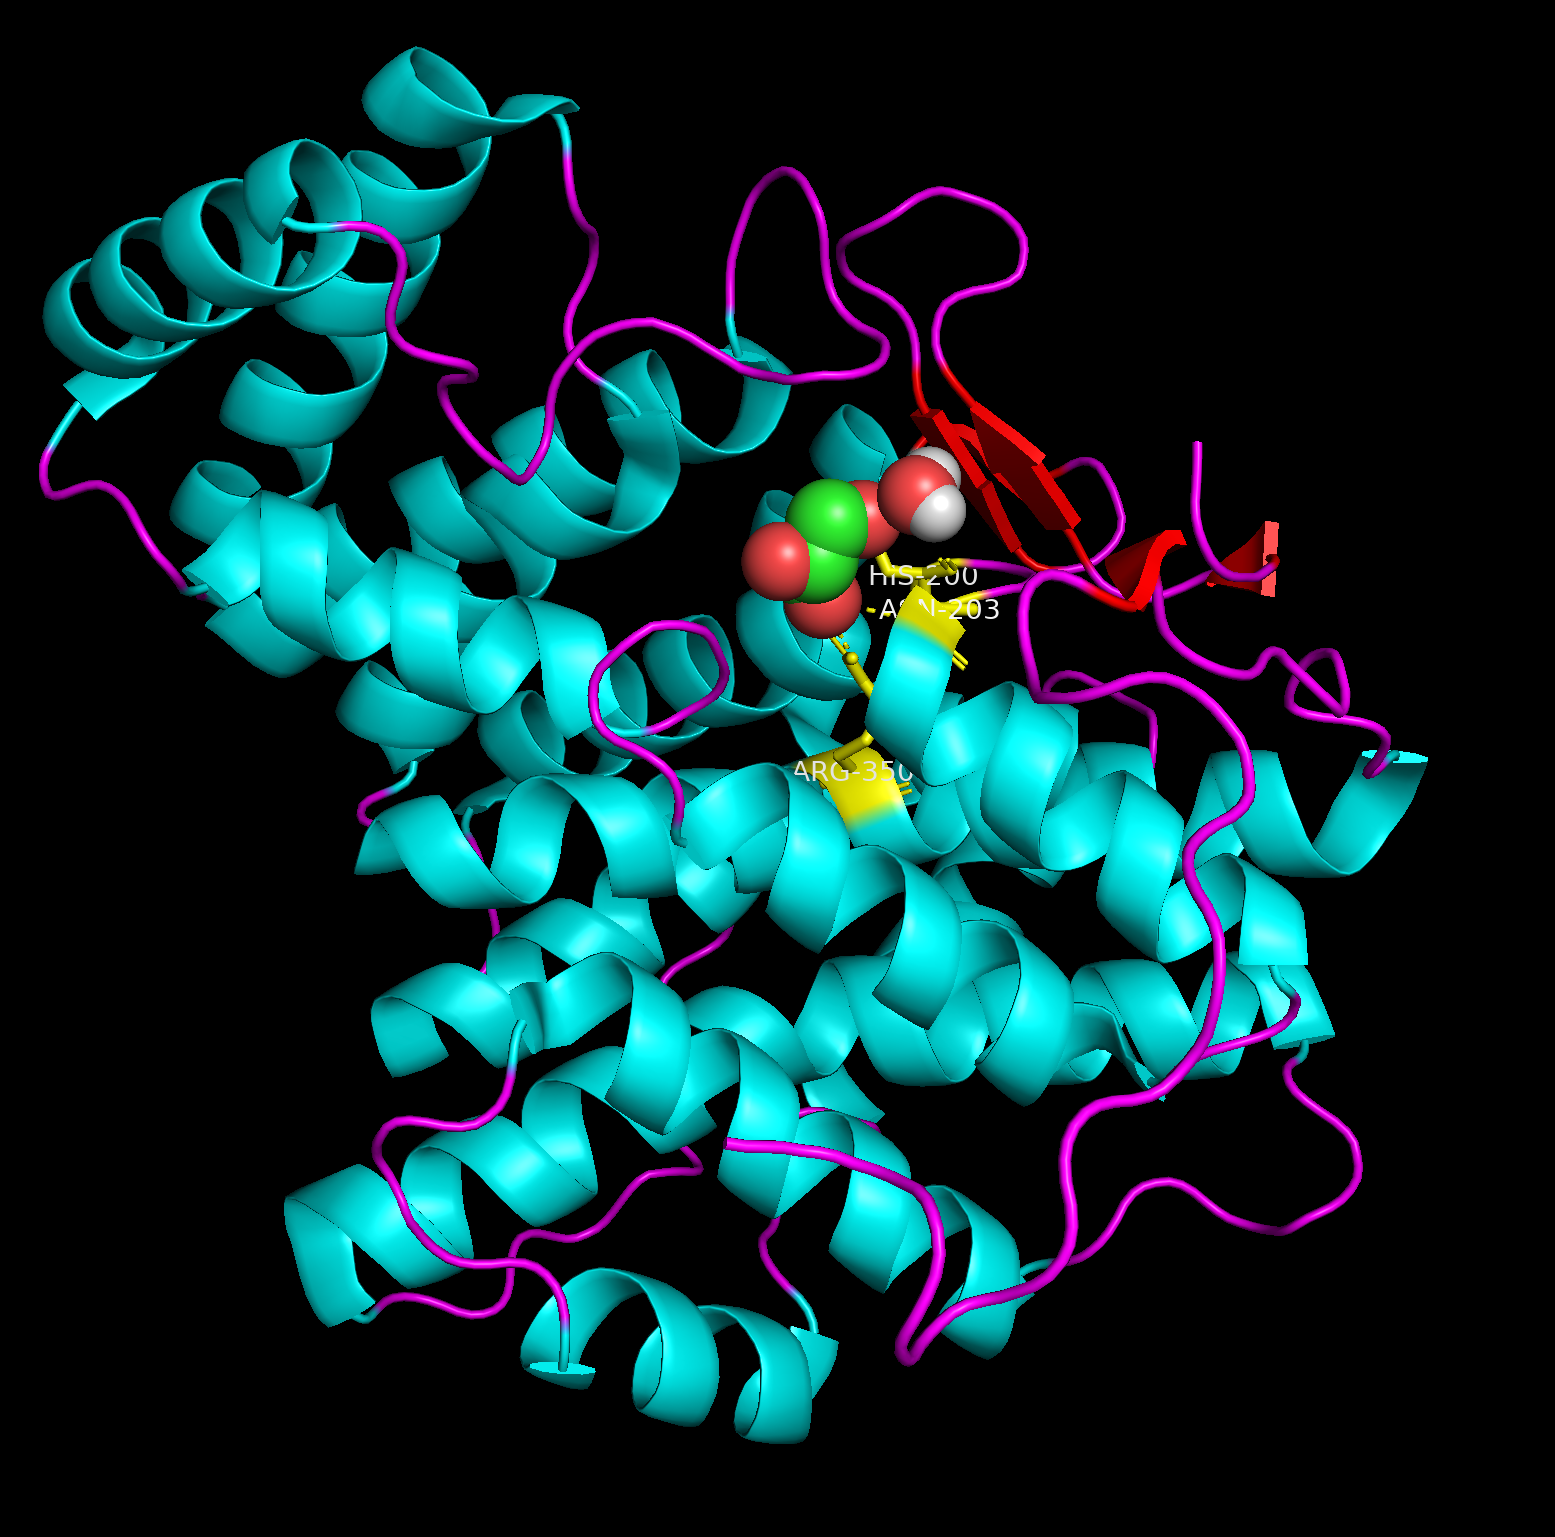
\includegraphics[width=0.9\textwidth]{Project 3/ligand.png}
	    \caption{Ligand interacting with residues. }
\end{figure}

\subsection{Protein Description}
2-methylcitrate synthase is a  key enzyme in the propionate metabolism pathway. It plays a crucial role in converting propionyl-CoA to 2-methylcitrate, this process is important in using propionate, as a scaffold to synthesizemethylcitrate, and it's particularly relevant in our bacteria, Escherichia coli.
The Structure was achieved trough a X-Ray Crystallography, a technique in which a beam of X-rays is directed at a crystal( repeated unit cell ). The crystal acts as a three-dimensional diffraction grating, scattering the X-rays in different directions. By analyzing the resulting diffraction pattern, scientists can mathematically reconstruct the arrangement of atoms within the crystal. because the angles and intensities of the diffracted X-rays provide information about the spatial distribution of electrons in the crystal lattice.
The resolution of the unit cell in Figure 3.4 is 0.241 nm ( or 2.41 Angstorms ).
In the figure we can recognize that the unit cell contains a complex of 10 subunits, each subunit represents only a single protein, they are displayed in different colours to enable better discrimination between subunits.
The small red dots are water molecules complexed with the protein, meaning that they are part of the fixed crystal lattice and should therefore not be considered mobile elements of the solvent, at best it can be used to compute the minimal hydrodynamic radius.
The complex is just a result of the energy minimization of steric constraints and hydrophic regions during the crystallization process, thus it does not indicate the in-vivo conditions of the protein.
The ligand
\begin{figure}[H]
        \centering
        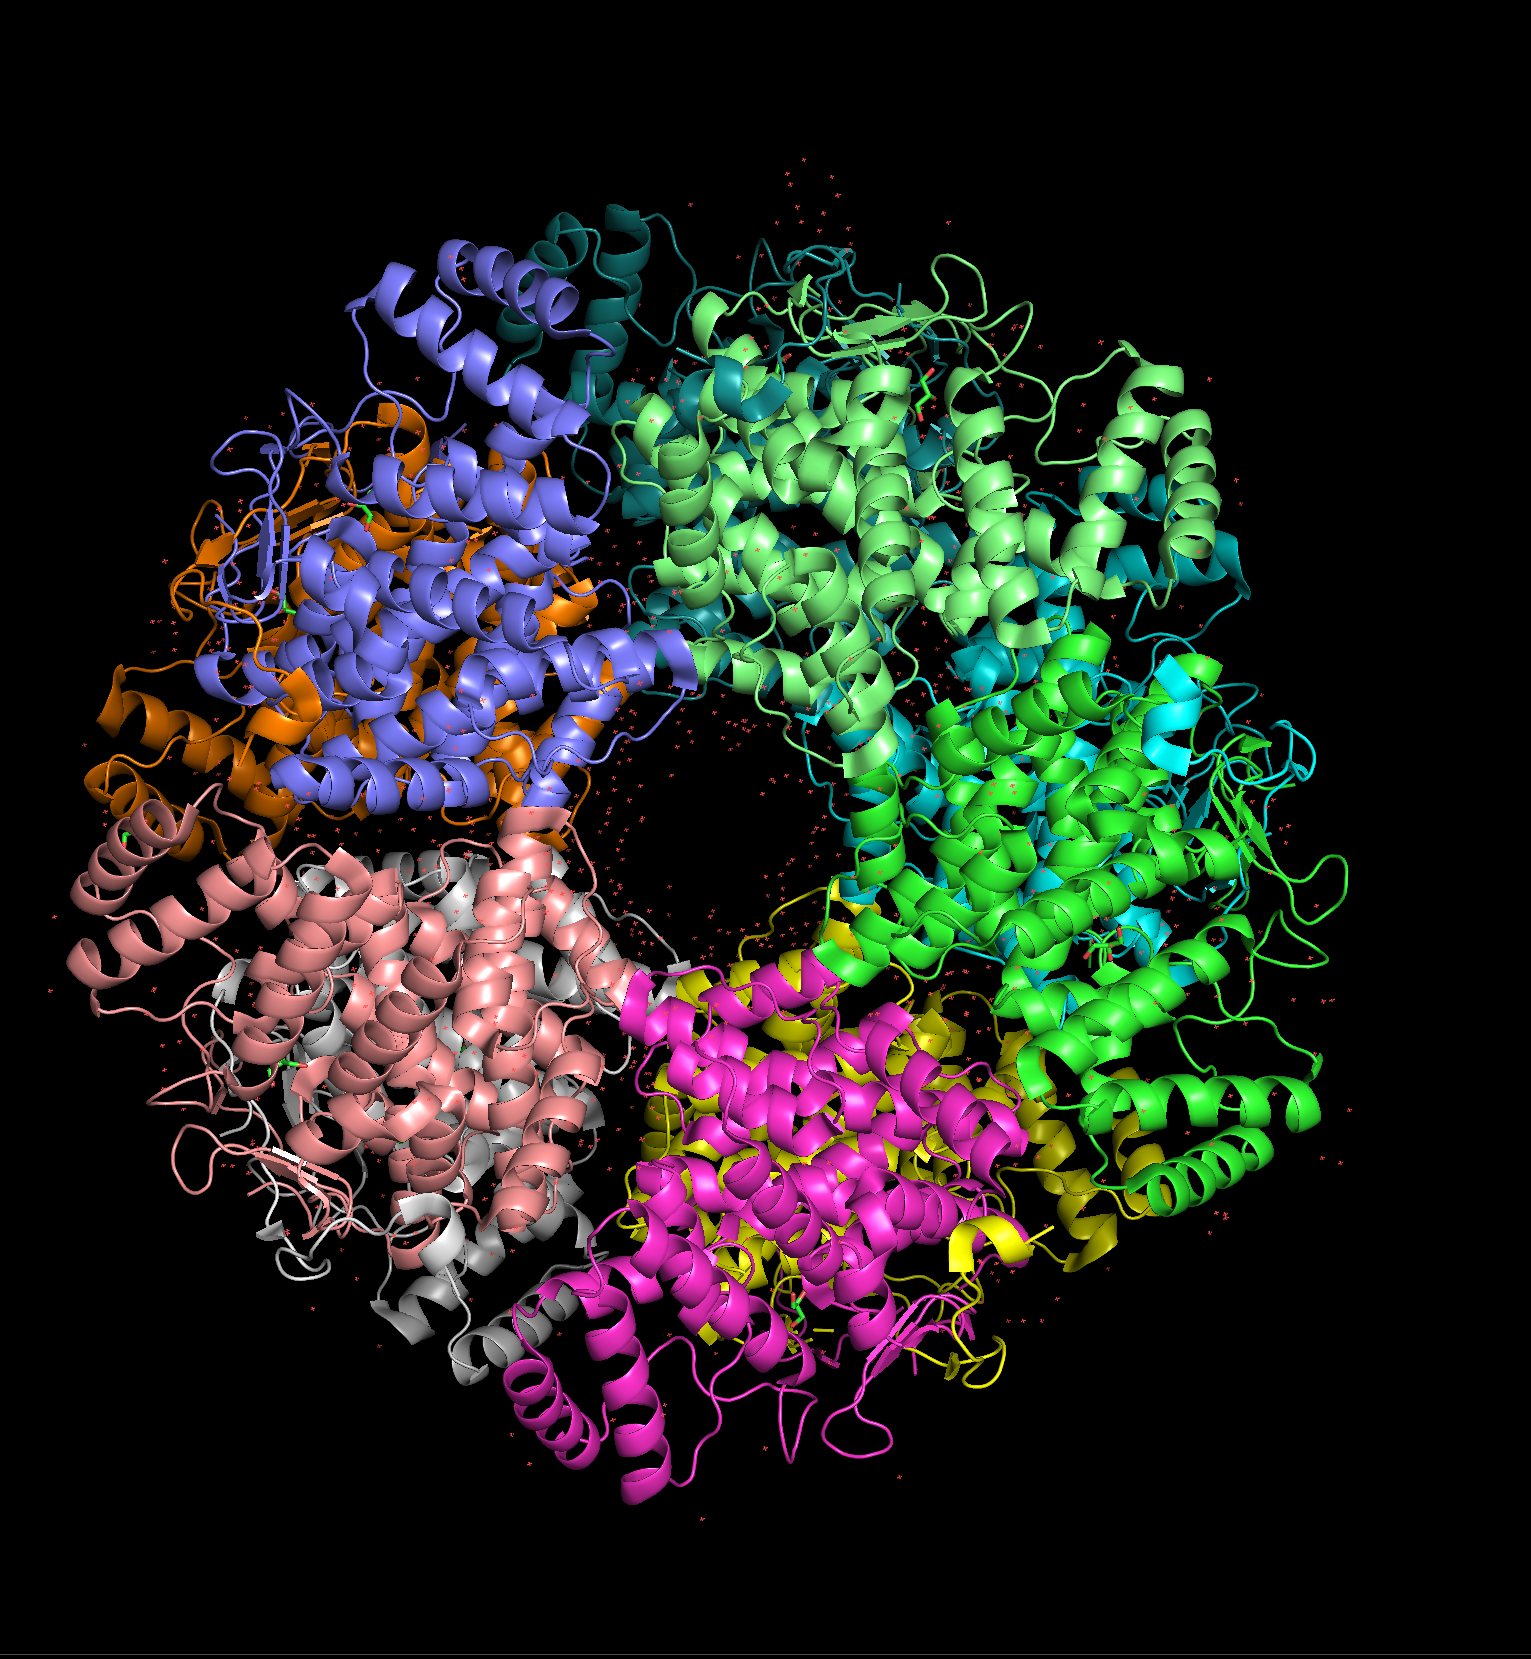
\includegraphics[width=0.7\textwidth]{Project 3/Repeating Cell X-ray Crystal.png}
	    \caption{Unit-cell of the protein crytsal}
\end{figure}
A note should be disclosed on the structure we studied: the crystal structure does not correspond to the same protein analyzed in the previous parts of our study.
The sequences analyzed in the previous parts of our study gave a putative belonging of our protein to E.Coli, the sequence of which corresponds to the prpC gene, where as the protein analyzed derives from the same highly conserved ( but not perfectly identical in sequence)  gene of the organism Salmonella Enterica.
The gene was transfected in E.Coli for better culture conditions but the protein sequence is still slightly different from the one we associated with our sample.
In Figure  3.3 we display the computed structure of our sequence by AlphaFold [\cite{jumper_highly_2021}] , we can say from a preliminary inspection that the two structures resemble each other very much, except for a region at the the C-terminus, which we can disregard as it seems to not be part of the enzymatic region of our protein.
\begin{figure}[H]
        \centering
        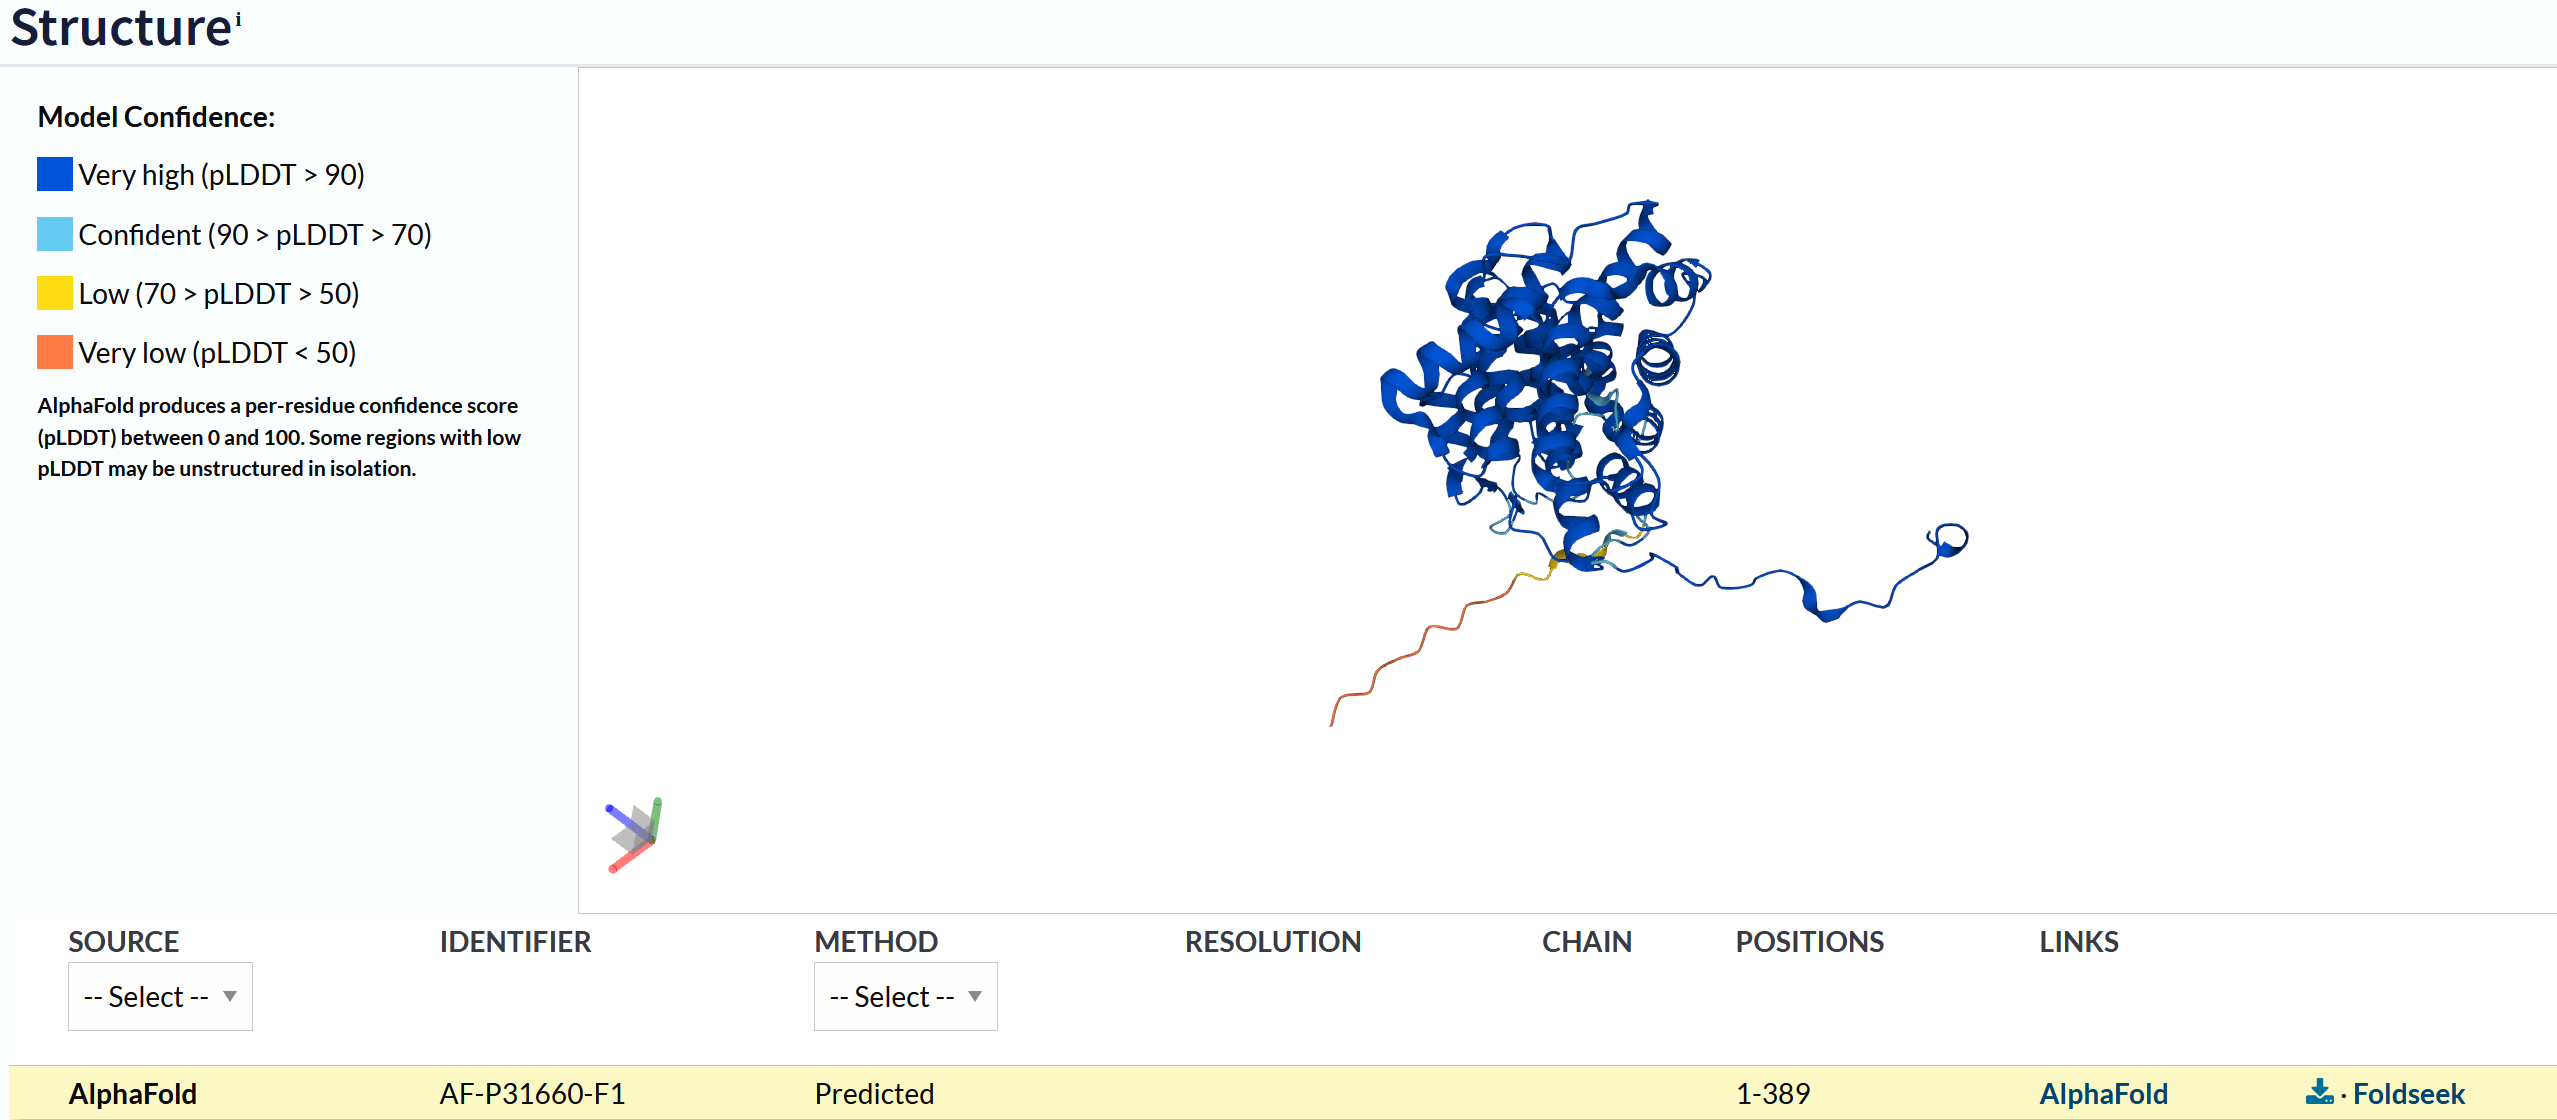
\includegraphics[width=0.9\textwidth]{Project 3/alphafold.png}
	    \caption{Alphafold prediction}
\end{figure}

In the following Figure 3.5, a summary of the relevant information regarding the crystal structure ,submitted to pdb, we used in our study is displayed.

\begin{figure}[H]
        \centering
        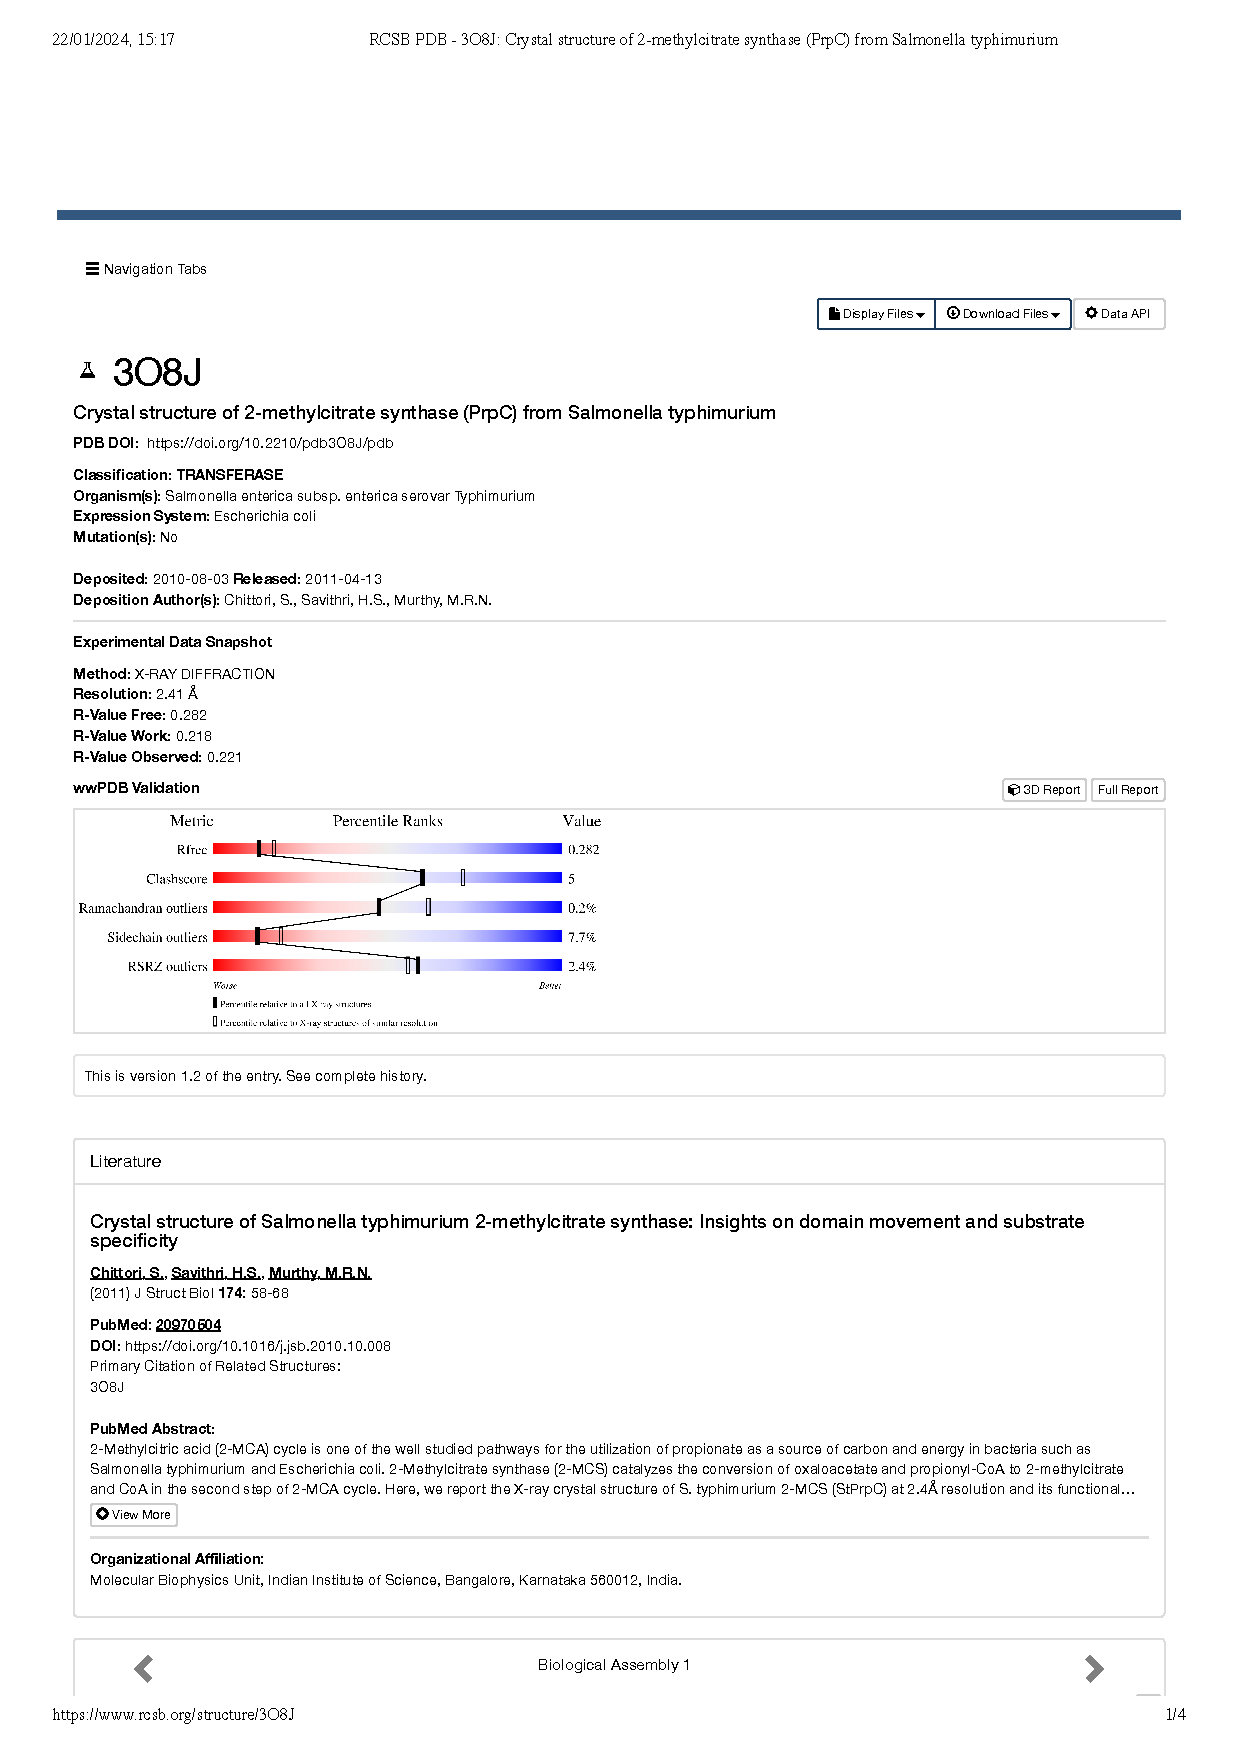
\includegraphics[width=0.9\textwidth]{Project 3/PDBreport.pdf}
	    \caption{ProteinDataBank Report}
\end{figure}




\section{discussions}

Considering the above mentioned details regarding the structured of our protein we can say that inspection of protein structures trough computational tools like Pymol [\cite{schrodinger_llc_pymol_2015}] or Chimera [\cite{pettersen_ucsf_2004}] provide great insight to the molecular functioning of proteins.
Such tools, and the various models and simulations they enable( which were not investigated in this study because of time constraints) are of great using at the cutting edge of drug development, interactomics and more generally to biophysics as a whole.

\chapter{Project 4}
This project focuses on exploring the enzymology of our protein trough the BRENDA database[CITATION].

\section{results}
The following results were found by searching 2-methylcitrate synthase in the BRENDA database and selecting the only result with an E.C. number of 2.3.3.5.



\subsection{The searching result from BRENDA database}

In the following picture, we can see the homepage of BRENDA which allows us to select a variety of information on our protein of interest.

\begin{figure}[H]
        \centering
        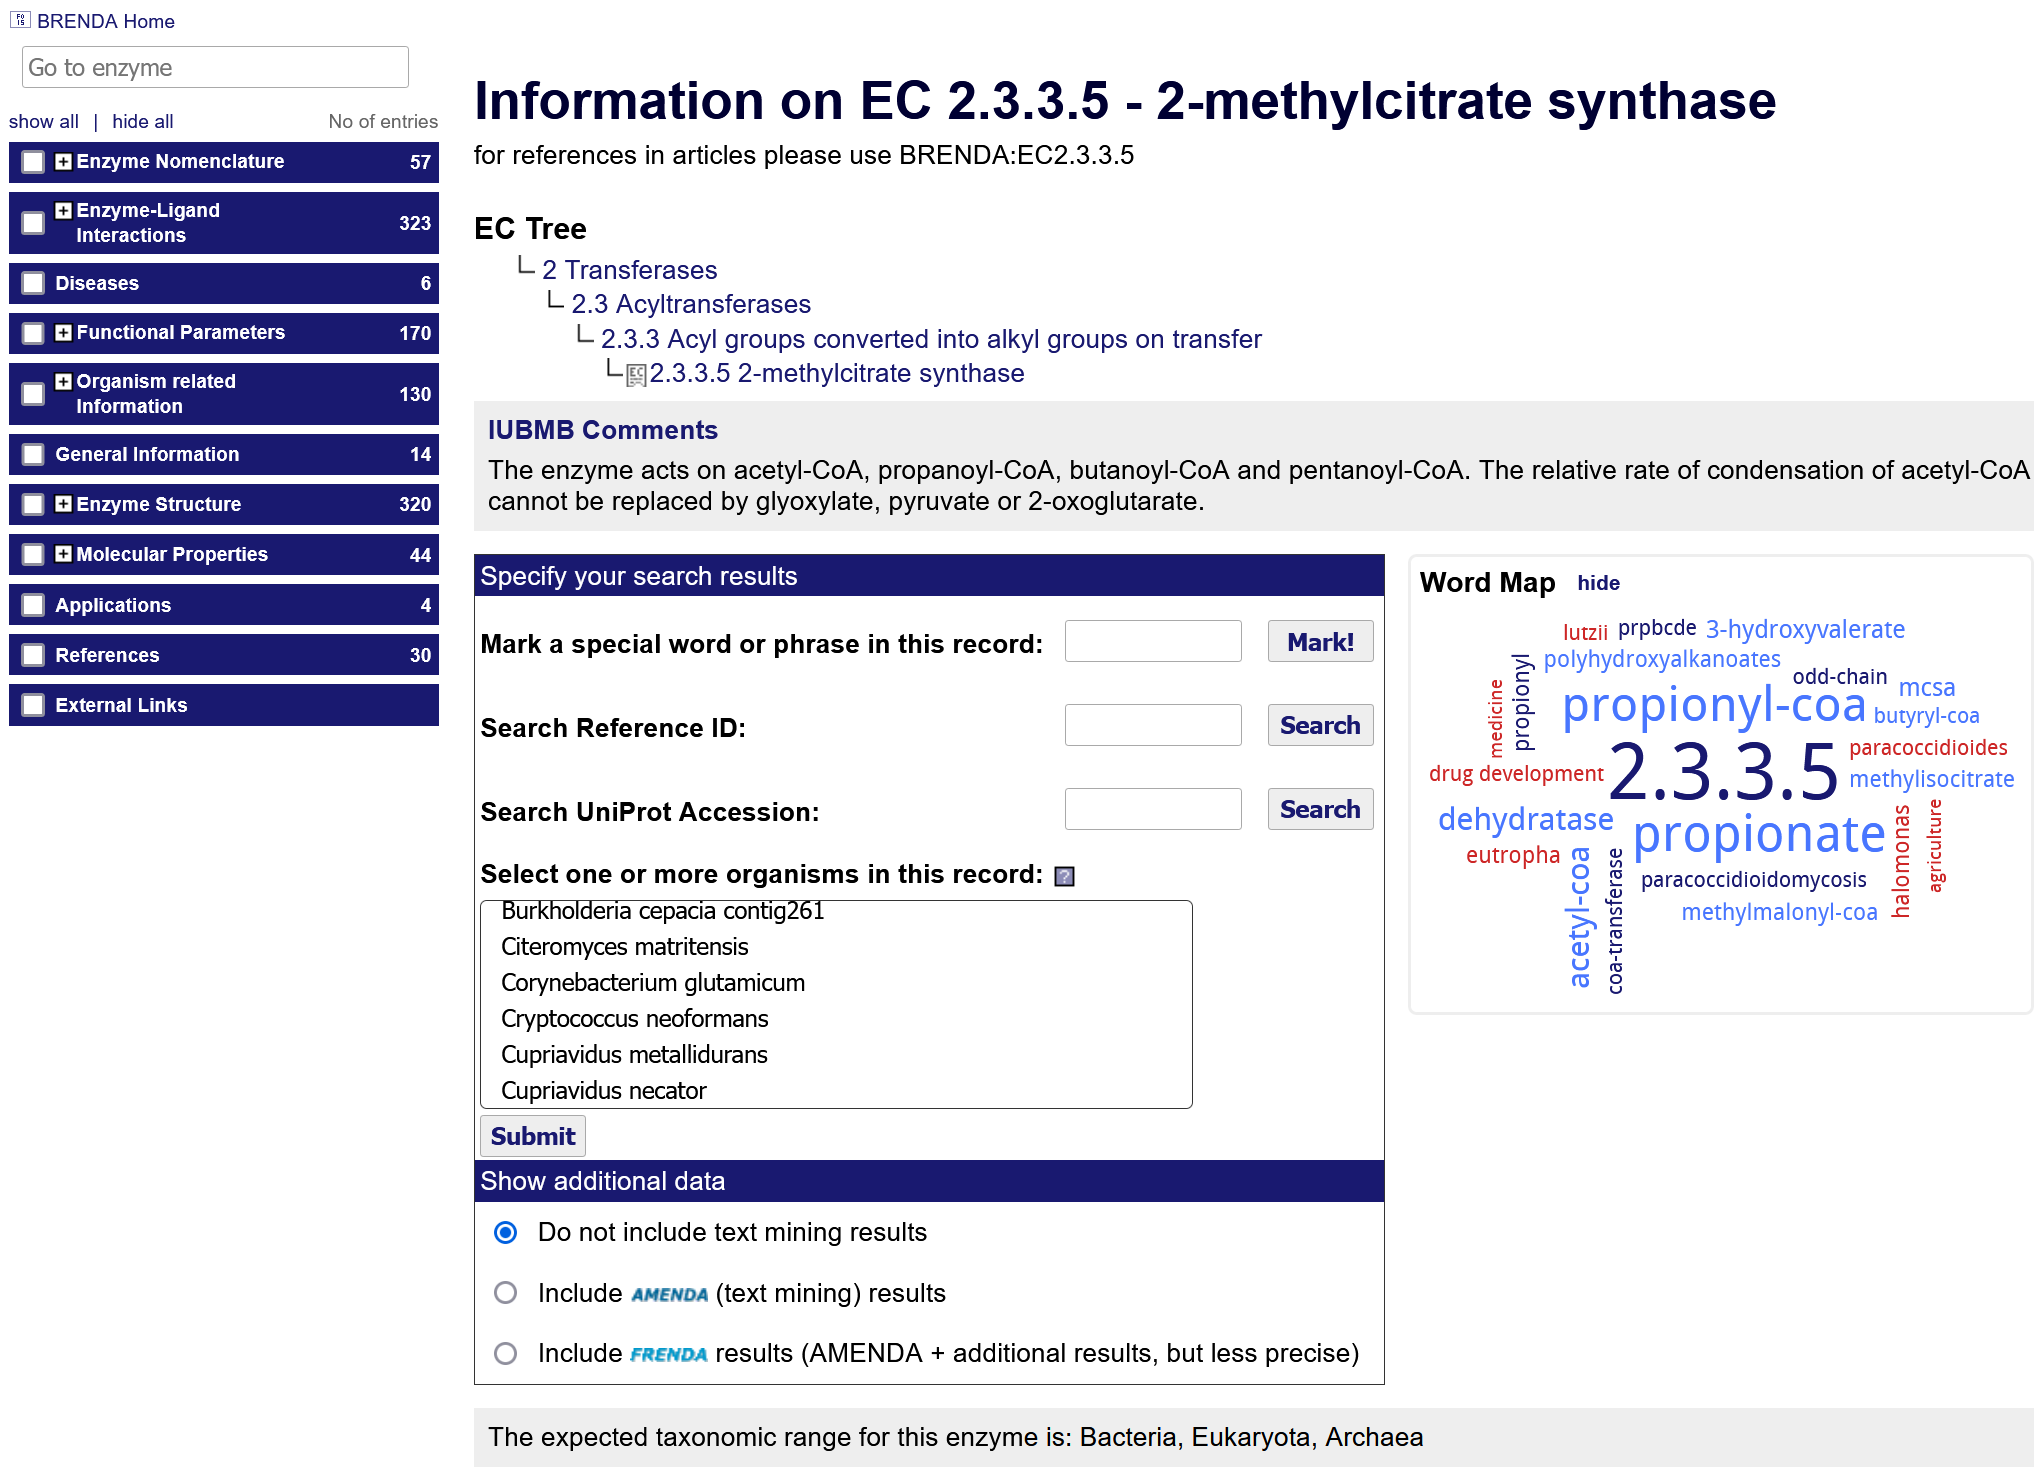
\includegraphics[width=0.9\textwidth]{Project 4/Brenda figures/image.png}
	    \caption{BRENDA Homepage}
\end{figure}

\begin{figure}
    \centering
    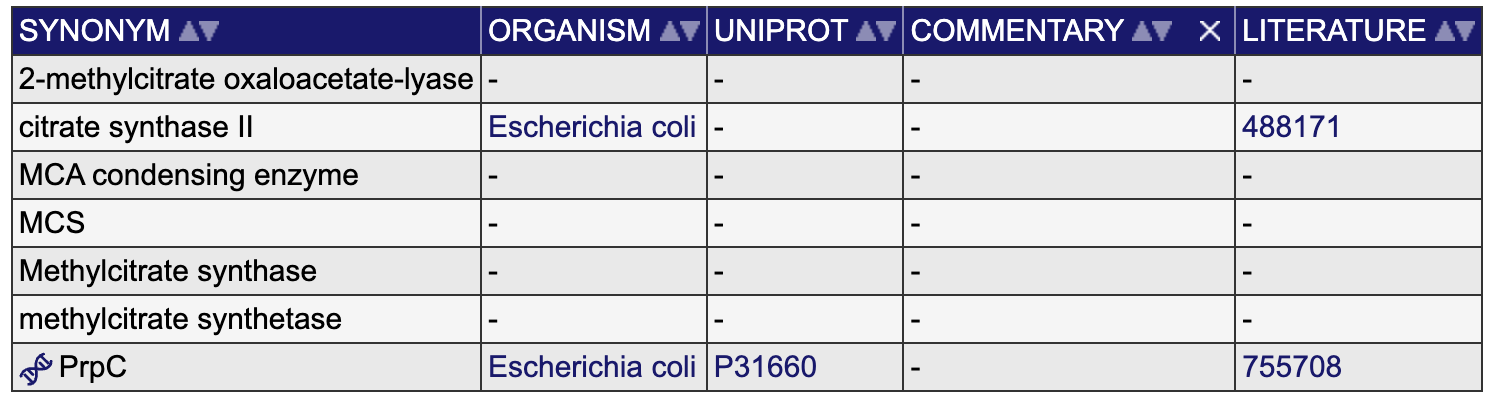
\includegraphics[width = 0.9\textwidth]{Project 4/Brenda figures/SYNONYM.png}
    \caption{Synonyms of 2-Methyl citrate synthase}
\end{figure}

\begin{figure}
    \centering
    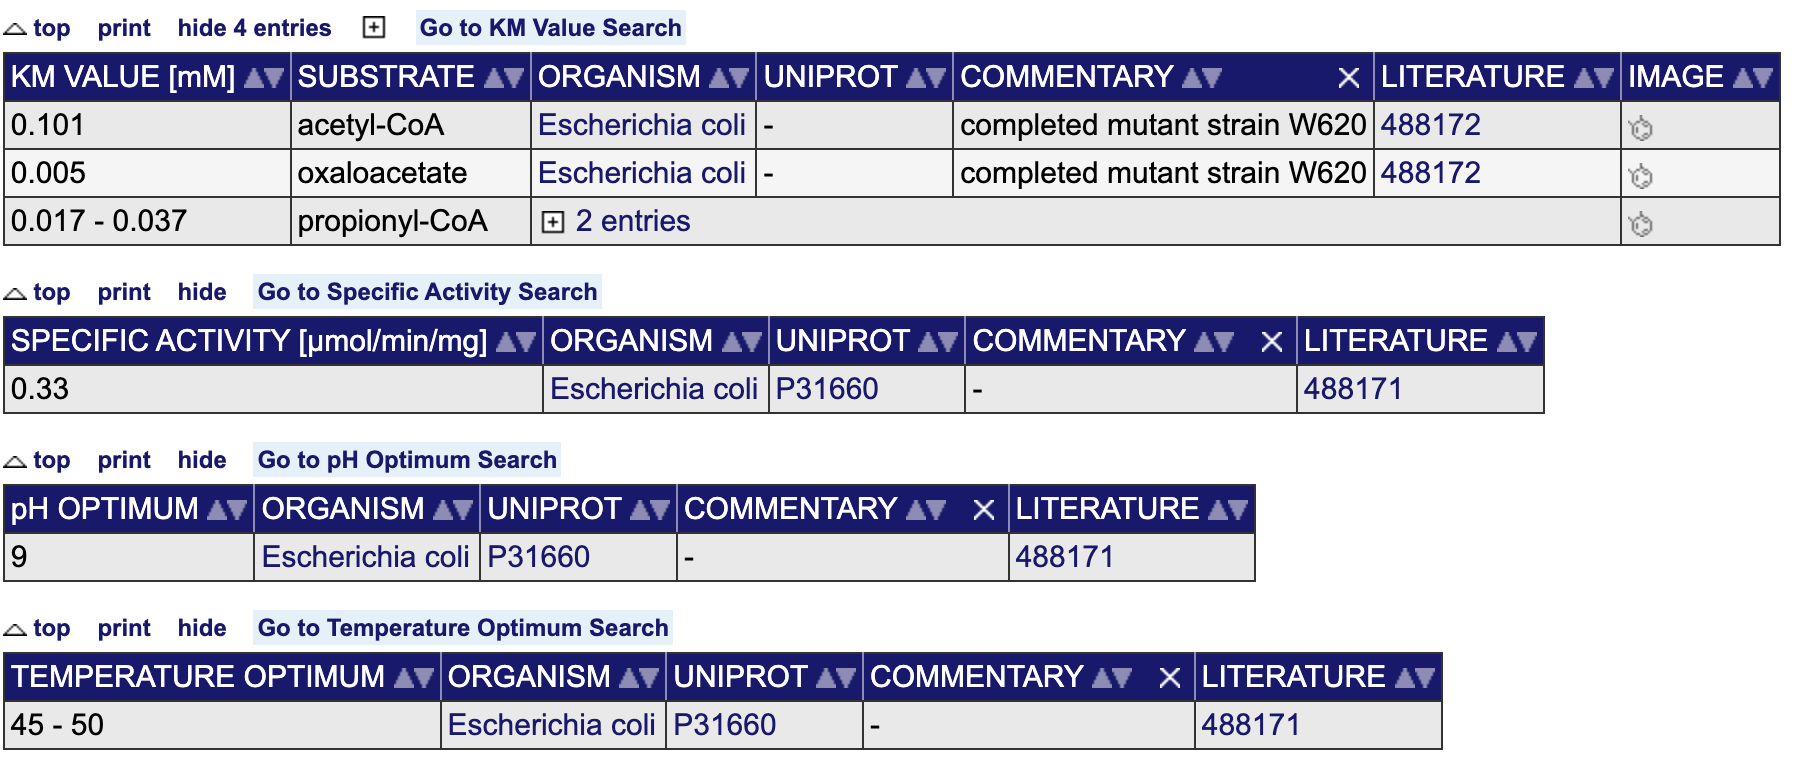
\includegraphics[width = 0.9\textwidth]{Project 4/Brenda figures/reaction conditions.png}
    \caption{Reaction conditions of 2-Methyl citrate synthase}
\end{figure}

\begin{figure}
    \centering
    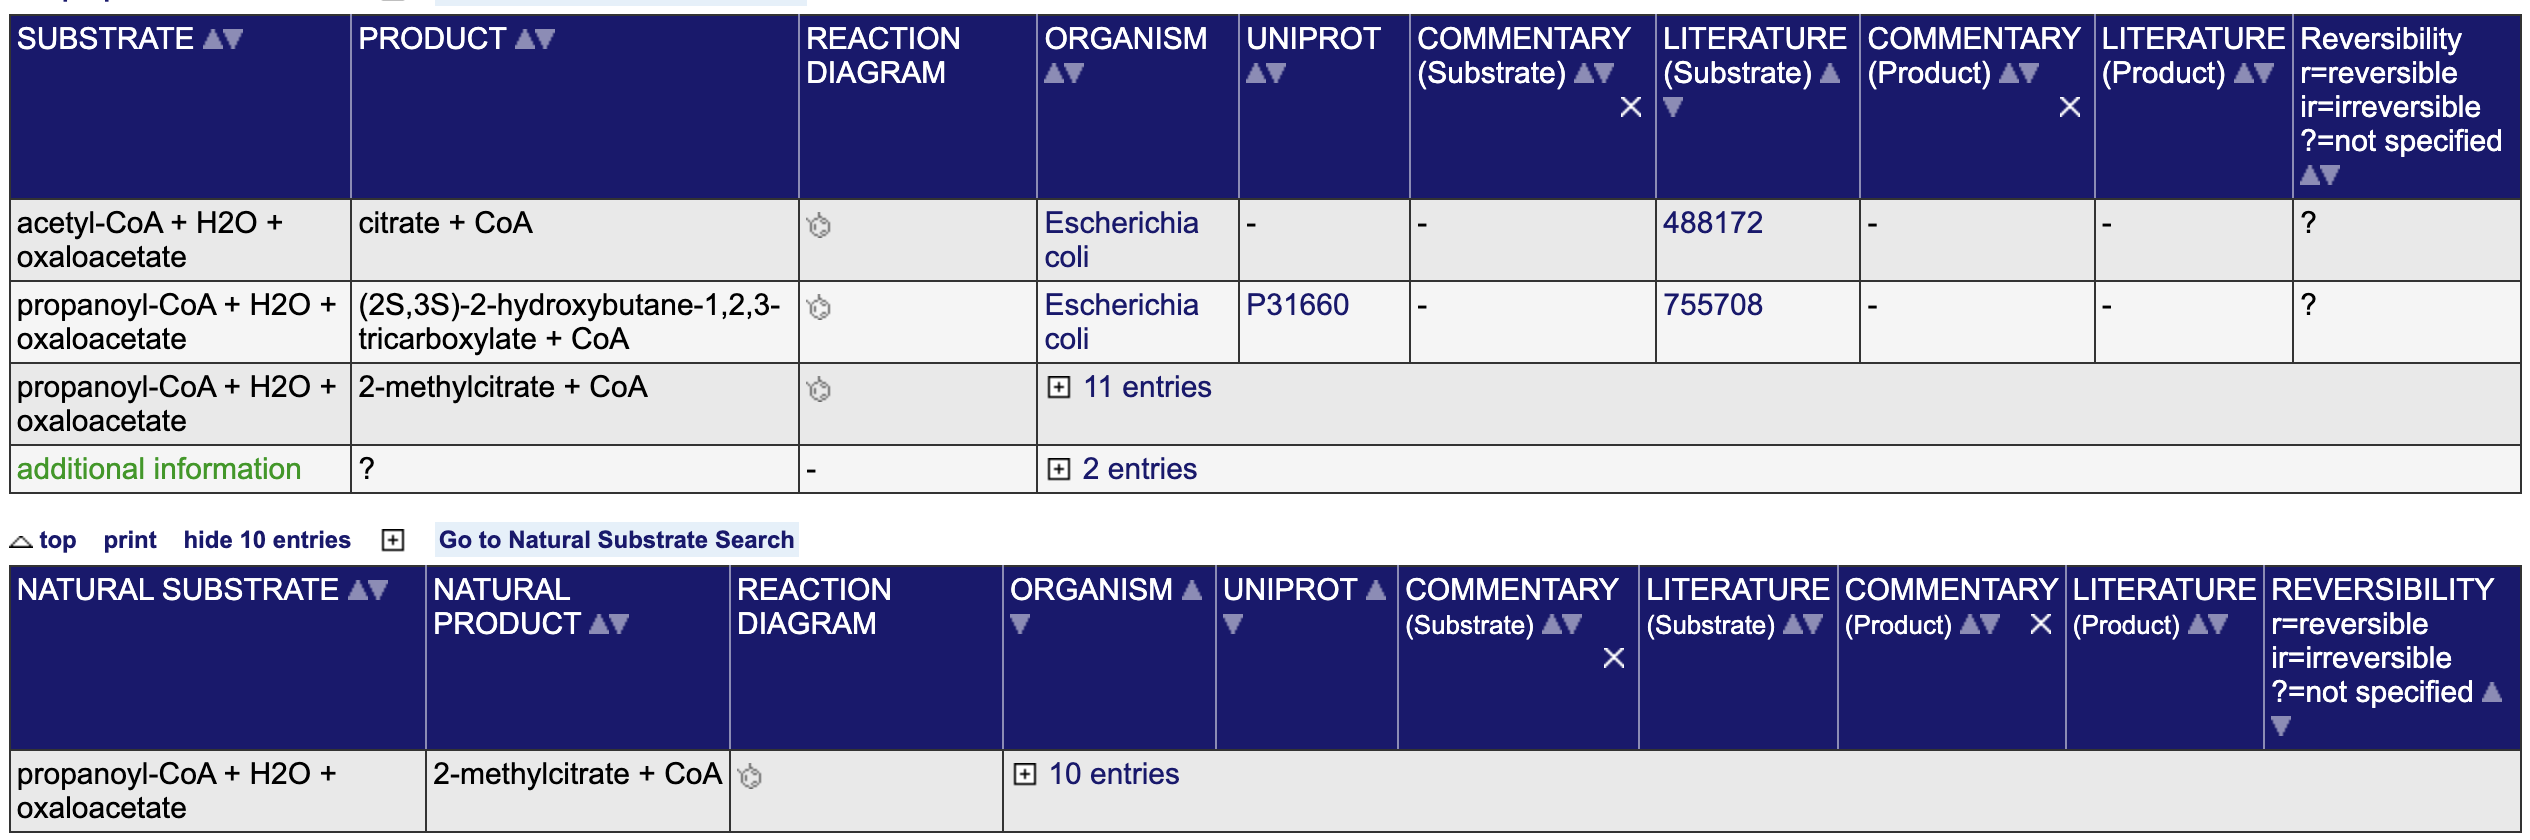
\includegraphics[width =0.9\textwidth]{Project 4/Brenda figures/substrates.png}
    \caption{Substrates related to the reactions of 2-Methyl citrate synthase}
\end{figure}

\begin{figure}
    \centering
    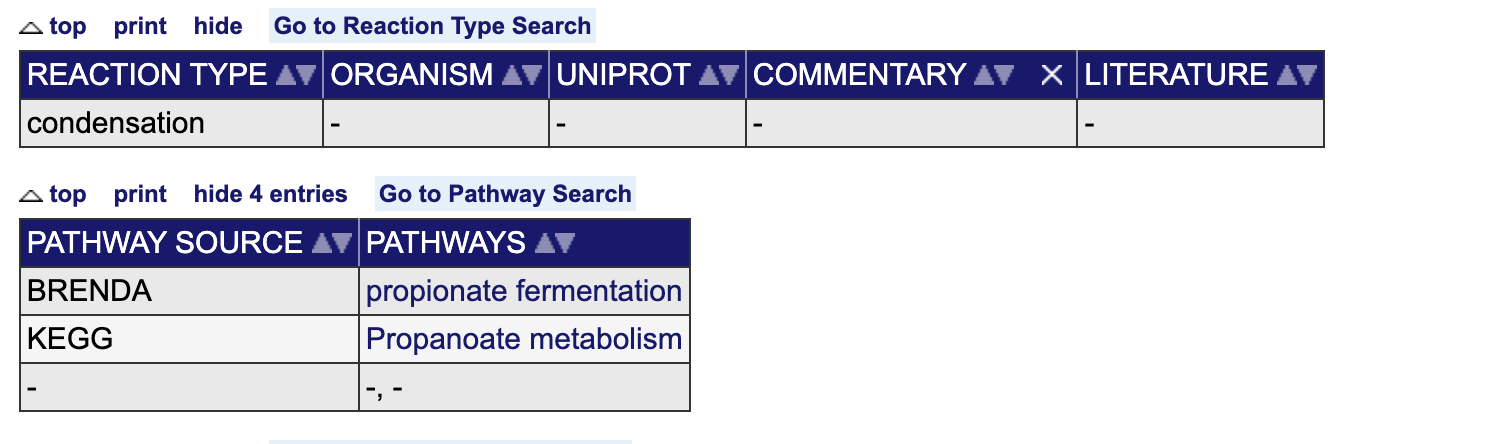
\includegraphics[width = 0.9\textwidth]{Project 4/Brenda figures/Reaction type and pathway source.png}
    \caption{Reaction types and pathway sources of 2-Methyl citrate synthase}
\end{figure}

\section{discussions}

a) The 3 substrates of this enzyme are propanoyl-CoA, H2O, and oxaloacetate, whereas its two products are (2R,3S)-2-hydroxybutane-1,2,3-tricarboxylate and CoA. This enzyme belongs to the family of transferases, specifically those acyltransferases that convert acyl groups into alkyl groups on transfer. The systematic name of this enzyme class is propanoyl-CoA:oxaloacetate C-propanoyltransferase (thioester-hydrolysing, 1-carboxyethyl-forming). Other names in common use include 2-methylcitrate oxaloacetate-lyase, MCS, methylcitrate synthase, and methylcitrate synthetase. This enzyme participates in propanoate metabolism.[\cite{chang_brenda_2021}] \\
%specific activity = Amount of Enzyme Activity/ Protein concentration

b) The measured ranges of activity displayed on BRENDA [\cite{chang_brenda_2021}] for pH are 5.5 to 10.5, the  analyzed temperature range is from 10 to 90 degrees.\\

c) The range of specific activity goes form 48 to 0.002, in particular for E.Coli it is 0.33.\\

d) The specific activity changes drastically between organisms. The variation in specific activity values for the same enzyme across different organisms can be attributed to several factors. Evolutionary adaptations play a crucial role, as enzymes undergo changes over time to meet the specific needs and environmental conditions of each organism. Substrate specificity is another factor, with organisms evolving enzymes tailored to their unique metabolic pathways.Optimal conditions, such as pH and temperature also influence enzyme activity, and organisms in different environments may express enzymes optimized for their specific habitats. Variations in metabolic pathways and the utilization of alternative substrates contribute to differences in enzyme specific activity. Additionally, the regulation of enzyme activity through feedback inhibition, allosteric regulation, and genetic control can vary among organisms. Genetic diversity within a species or population further adds to the variability in enzyme properties. Different strains or individuals may express slightly different forms of an enzyme, leading to differences in specific activity. In essence, the diversity in specific activity values reflects the intricate interplay of evolutionary, environmental, and genetic factors shaping biochemical processes in various biological systems.\\

e) The range of the KM for acetyl-CoA is from 0.00126 to 0.35 1/mMs-1\\

f) The pH optimum  relates to the enzyme mechanism and structure because enzyme structure is directly related to the pH of the solution around it, different pH could cause the enzyme to unfold or to increase the hydrophobicity of the enzyme making it structurally immobile. This results in a change of the efficiency of the enzyme .\\

g)  3,3-thiodipropionic acid and 3-phosphonopropionic acid are competitive inhibitors with a similar structure to the substrate which is oxoloacetate.\\


\chapter{Project 5}

\section{results}
In this project, we generated five homologs of 2-Methyl citrate synthase from PDB and ENZYME. We appied Cluster Omega to compare the conserved sequences among the homologs, and plotted the 3-D structure of 2-Methyl citrate synthase labeled by conservation posibility, to see the relationship between conserved sequences and protein structure.

\subsection{homologs of 2-Methyl citrate synthases}

Searching from the database, we found five homologs of the 2-Methyl citrate synthases in ecoli, which are 2-methylcitrate synthase|Salmonella enterica (90371), Citrate synthase|Pseudomonas aeruginosa PAO1 (208964), Methylcitrate synthase|Mycobacterium tuberculosis (83332), 2-methylcitrate synthase|Coxiella burnetii (777) and 2-methylcitrate synthase, mitochondrial|Neosartorya fumigata (strain CEA10 / CBS 144.89 / FGSC A1163) (451804).

\subsection{Comparing the homologs using ClustalOmega(figure 5.1 and 5.2)}

\begin{figure}
    \centering
    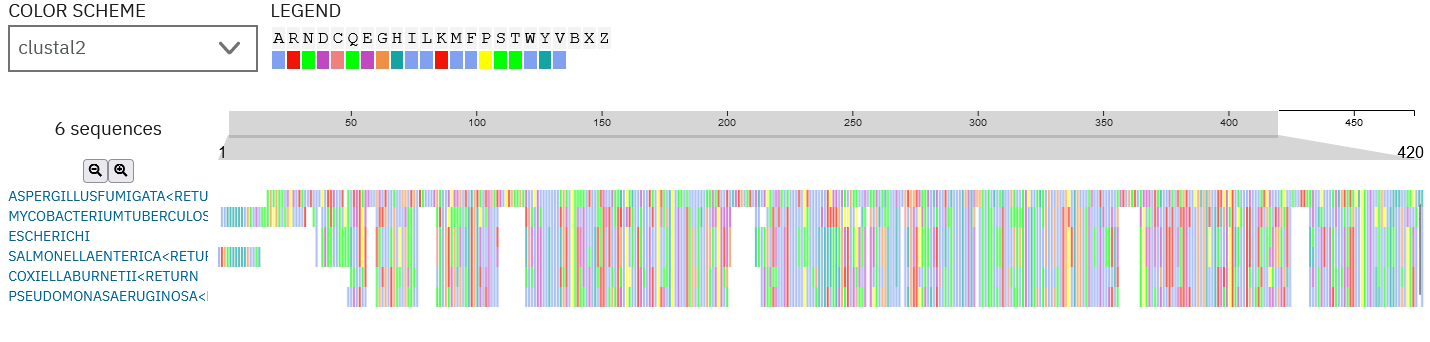
\includegraphics[width = 0.9\textwidth]{Project 5/clustalo_image_summary.png}
    \caption{The overview of the sequences among the homologs.}
\end{figure}

\begin{figure}
    \centering
    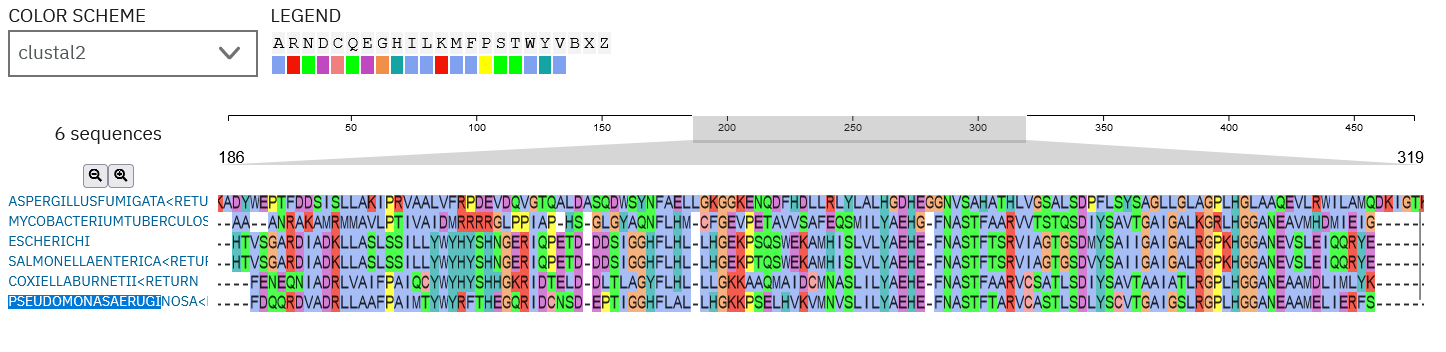
\includegraphics[width = 0.9\textwidth]{Project 5/clustalo_image_detailed.png}
    \caption{The highly conserved sequences area among the homologs}
\end{figure}

\subsection{The 3D image showing the highly conserved regions(figure 5.3)}

\begin{figure}
    \centering
    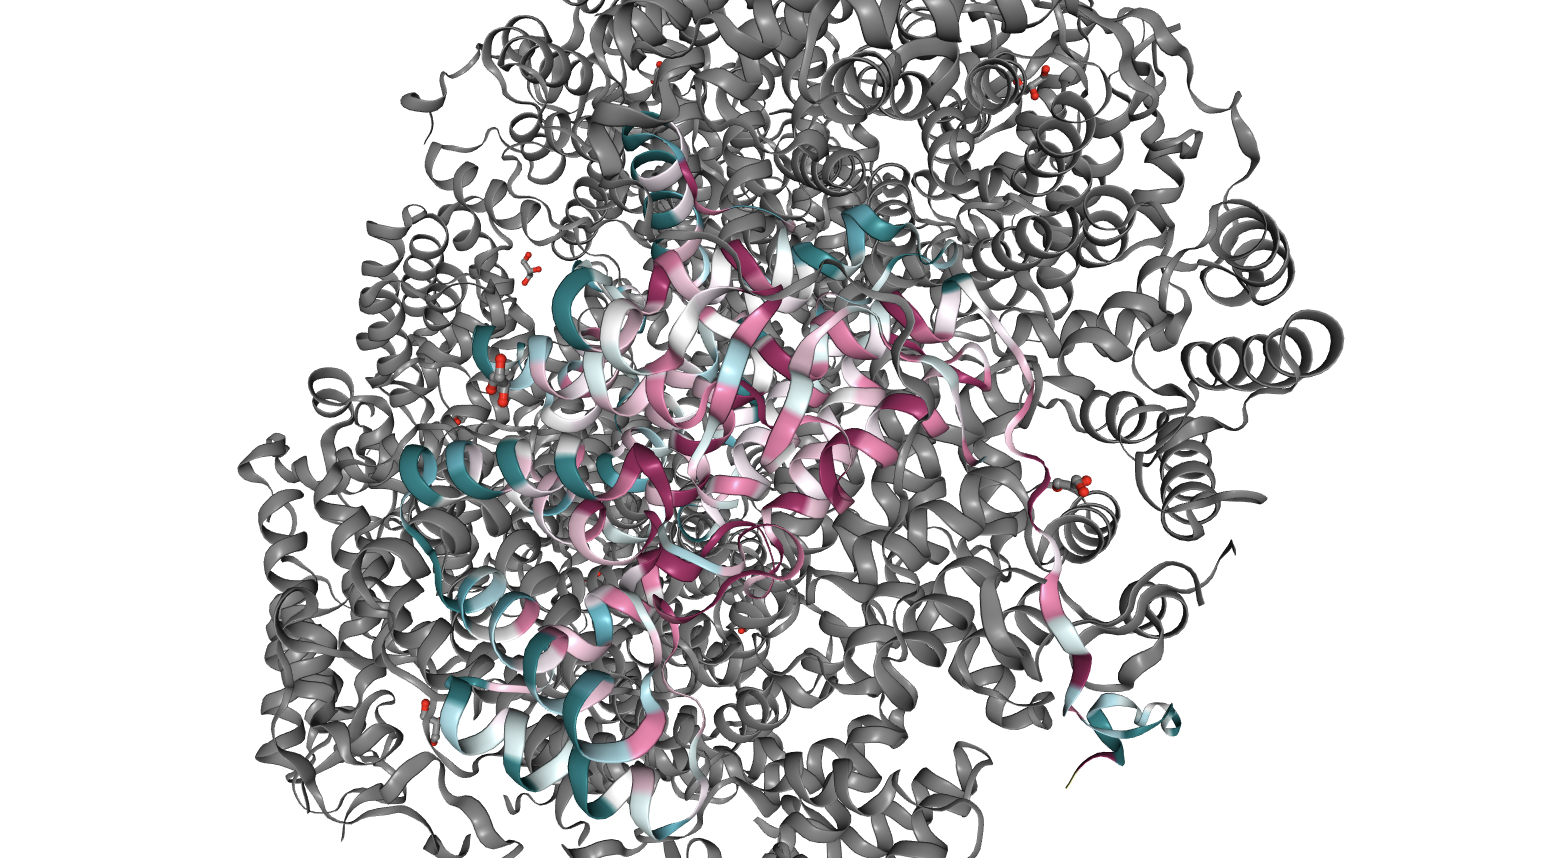
\includegraphics[width = 0.9\textwidth]{Project 5/differences/differences.png}
    \caption{The conserved part(red) and the variable part(green) of the enzyme}
\end{figure}

\section{discussions}

\begin{figure}
    \centering
    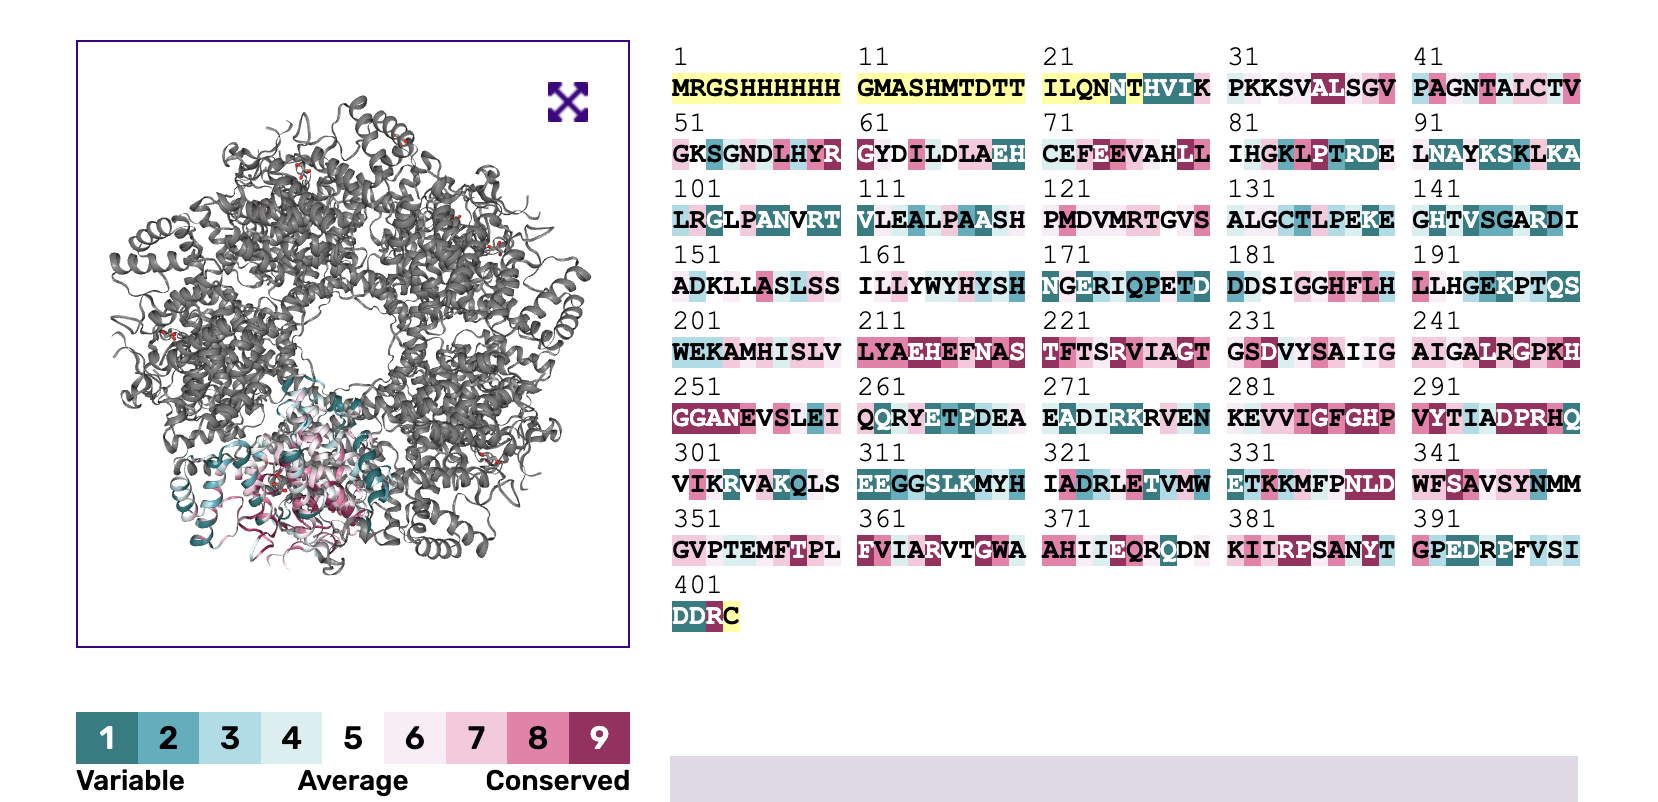
\includegraphics[width = 0.9\textwidth]{Project 5/Consurf image/consurf.png}
    \caption{The conserved sequences of 2-Methyl citrate synthase chain A, generated by Consurf}
\end{figure}

a) An * (asterisk) indicates positions which have a single, fully conserved residue; a : (colon) indicates conservation between groups of strongly similar properties, roughly equivalent to scoring > 0.5 in the Gonnet PAM 250 matrix; A . (period) indicates conservation between groups of weakly similar properties, roughly equivalent to scoring =< 0.5 and > 0 in the Gonnet PAM 250 matrix.\\%\cite{AlignmentResults}


b) The results generated from Consurf show the possibility of conservation for each amino-acid(Figure 5.4), while the results of Clustal Omega directly display the sequences of differenet homologs, while the users can find the conserved sequences by themselves. Moreover, the Consurf results only illustrate the possibility on each individual amino acid, while the Clustal Omega computations display the full conserved sequences. \\


%sequence conservation means that the sequence may exists in different proteins because it is necessary(have good functions?)
c)Yes. While observing the primary sequences and the amino acid conservation, we noticed that there are some special amino acid sequences that are highly similar among the homologs, some sequences are similar among several homologs, but not all, while some sequences are highly random between different homologs. Similar sequences appear mainly between the amino acid numbers 200 to 350.\\


%sequence motif: a set of conserved amino acid residues that are important for protein function and are located within a certain distance from each other.
d) A sequence motif is a set of conserved amino acid residues that are important for protein function and are loacted within a certain distance from each other%\cite{SequneceMotif}
. The conserved sequence motif means that the sequnece motif is based on conserved sequences. \\
An analysis tool called EMBOSS CONs is applied to find the specific conserved sequence motif. With the input of five homologs sequences, the comparing results are shown in the figure 5.5. In the results, for example, sequence 'kiaals' exists in all homologs, which means that it's highly probable for 'kiaals' be a conserved sequence motif.\\

\begin{figure}
    \centering
    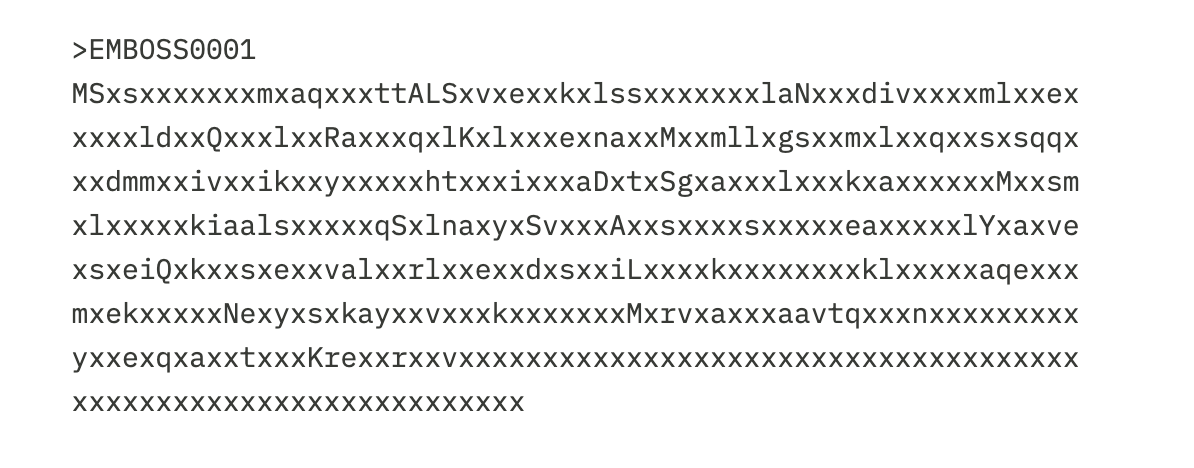
\includegraphics[width = 0.9\textwidth]{Project 5/Sequence images/sequence.png}
    \caption{the conserved sequence motif generated by EMBOSS CONs.}
\end{figure}

e) As is shown in the figure 5.3, compared to the more variable parts, most conserved sequences are located at the center part of the chain. Besides, the shape of conserved sequences are basically standard alpha helices and beta sheets, while the variable parts are more random.\\

\printbibliography
\end{document}